

%------------------------------------------------------------------------
%
%    Copyright (C) 1985-2020  Georg Umgiesser
%
%    This file is part of SHYFEM.
%
%    SHYFEM is free software: you can redistribute it and/or modify
%    it under the terms of the GNU General Public License as published by
%    the Free Software Foundation, either version 3 of the License, or
%    (at your option) any later version.
%
%    SHYFEM is distributed in the hope that it will be useful,
%    but WITHOUT ANY WARRANTY; without even the implied warranty of
%    MERCHANTABILITY or FITNESS FOR A PARTICULAR PURPOSE. See the
%    GNU General Public License for more details.
%
%    You should have received a copy of the GNU General Public License
%    along with SHYFEM. Please see the file COPYING in the main directory.
%    If not, see <http://www.gnu.org/licenses/>.
%
%    Contributions to this file can be found below in the revision log.
%
%------------------------------------------------------------------------

% $Id$

\documentclass{report}
%\documentclass[draft]{report}

\usepackage{a4}
\usepackage{shortvrb}
\usepackage{pslatex}
\usepackage{xcolor} %DEB
\usepackage{graphicx}
\usepackage{verbatim}
\usepackage{alltt}		% as verbatim, but interpret \ { }
\usepackage{amsmath, amssymb}

\newenvironment{code}{\verbatim}{\endverbatim}
\newenvironment{codem}{\alltt}{\endalltt}	%interpret \
\newcommand{\ttt}[1]{{\tt #1}}

\newcommand{\shy}{{\tt SHYFEM}}
\newcommand{\shyfem}{{\tt SHYFEM}}
\newcommand{\psp}{{\tt SHYFEM}}

%\input{P_version.tex} %DEB scommentare
\newcommand{\VERSION}{DUMMY} %DEB dummy
\newcommand{\version
}{DUMMY} %DEB dummy
\newcommand{\shyname}{shyfem-\version}
%\newcommand{\shydist}{\shyname.tar.gz} %DEB scommentare
\newcommand{\shydist}{\shyfem-DUMMY.tar.gz} %DEB dummy
\newcommand{\basedir}{/home/model}
\newcommand{\shydir}{\basedir/shyfem-\version}

\newcommand{\descrpsep}{\vspace{0.2cm}}
\newcommand{\descrpitem}[1]{\descrpsep\parbox[t]{2cm}{#1}}
\newcommand{\descrptext}[1]{\parbox[t]{8cm}{#1}\descrpsep}
\newcommand{\descrp}[1]{\descrpsep\parbox[t]{4cm}{#1}}
\newcommand{\descrpn}[1]{\parbox[t]{4cm}{#1}}

\newcommand{\densityunit}{kg\,m${}^{-3}$}
\newcommand{\accelunit}{m\,s${}^{-2}$}
\newcommand{\maccelunit}{m${}^{4}$\,s${}^{-2}$}
\newcommand{\dischargeunit}{m${}^3$\,s${}^{-1}$}

\newcommand{\ten}[1]{$\cdot 10^{#1}$}
\newcommand{\degrees}{${}^o$}

\newcommand{\figref}[1]{\ref{fig:#1}}
\newcommand{\Fig}{Fig.~}

\newcommand{\todo}[1]{This section still has to be written by #1}

\parindent 0cm

\newcommand{\importstr}[2]{%
\begin{figure}
\begin{alltt}
\input{#1.str}
\end{alltt}
\caption{#2}
\label{fig:#1}
\end{figure}
}

\MakeShortVerb{\|}

\hyphenation{ ba-thy-me-try stop-ped sim-u-la-ted }

%%%%%%%%%%%%%%%%%%%%%%%%%%%%%%%%%%%%%%%%%%%%%%%%%%%%%%%%% front matter

\title{%
	\shy{}
	\\Finite Element Model for Coastal Seas
	\\~
	\\User Manual
	}

\author{%
	The SHYFEM Group
	\\Georg Umgiesser
	\\Oceanography, ISMAR-CNR
	\\Arsenale Tesa 104, Castello 2737/F
	\\30122 Venezia, Italy
	\vspace{0.5cm}
	\\georg.umgiesser@ismar.cnr.it
	\vspace{1cm}
	\\Version \VERSION
	}

%\address{ISDGM-CNR}

%\date{}		%uncomment for no date

%%%%%%%%%%%%%%%%%%%%%%%%%%%%%%%%%%%%%%%%%%%%%%%%%%%%%%%%% document

\begin{document}

\bibliographystyle{plain}

\pagenumbering{roman}
\pagestyle{plain}

\maketitle

%\begin{abstract}
% to be written
%\end{abstract}

\thispagestyle{empty}

\newpage
\tableofcontents
\newpage

%%%%%%%%%%%%%%%%%%%%%%%%%%%%%%%%%%%%%%%%%%%%%%%%%%%%%%%%%%%%%%%%%%%%%%%%
%%%%%%%%%%%%%%%%%%%%%%%%%%%%%%%%%%%%%%%%%%%%%%%%%%%%%%%%%%%%%%%%%%%%%%%%
%%%%%%%%%%%%%%%%%%%%%%%%%%%%%%%%%%%%%%%%%%%%%%%%%%%%%%%%%%%%%%%%%%%%%%%%

\chapter*{Disclaimer}
	\addcontentsline{toc}{chapter}{Disclaimer}

	
%------------------------------------------------------------------------
%
%    Copyright (C) 1985-2020  Georg Umgiesser
%
%    This file is part of SHYFEM.
%
%    SHYFEM is free software: you can redistribute it and/or modify
%    it under the terms of the GNU General Public License as published by
%    the Free Software Foundation, either version 3 of the License, or
%    (at your option) any later version.
%
%    SHYFEM is distributed in the hope that it will be useful,
%    but WITHOUT ANY WARRANTY; without even the implied warranty of
%    MERCHANTABILITY or FITNESS FOR A PARTICULAR PURPOSE. See the
%    GNU General Public License for more details.
%
%    You should have received a copy of the GNU General Public License
%    along with SHYFEM. Please see the file COPYING in the main directory.
%    If not, see <http://www.gnu.org/licenses/>.
%
%    Contributions to this file can be found below in the revision log.
%
%------------------------------------------------------------------------

\begin{quotation}

   Copyright (c) 1992-2012 by Georg Umgiesser

   Permission to use, copy, modify, and distribute this software
   and its documentation for any purpose and without fee is hereby
   granted, provided that the above copyright notice appear in all
   copies and that both that copyright notice and this permission
   notice appear in supporting documentation.

   This file is provided AS IS with no warranties of any kind.
   The author shall have no liability with respect to the
   infringement of copyrights, trade secrets or any patents by
   this file or any part thereof.  In no event will the author
   be liable for any lost revenue or profits or other special,
   indirect and consequential damages.

   Comments and additions should be sent to the author:

        \begin{verbatim}
                      Georg Umgiesser                                  
                      Oceanography, ISMAR-CNR
                      Arsenale Tesa 104, Castello 2737/F
                      30122 Venezia
                      Italy

                      Tel.   : ++39-041-2407943
                      Fax    : ++39-041-2407940
                      E-Mail : georg.umgiesser@ismar.cnr.it
        \end{verbatim}
\end{quotation}



\newpage
\pagenumbering{arabic}

%%%%%%%%%%%%%%%%%%%%%%%%%%%%%%%%%%%%%%%%%%%%%%%%%%%%%%%%%%%%%%%%%%%%%%%%
%%%%%%%%%%%%%%%%%%%%%%%%%%%%%%%%%%%%%%%%%%%%%%%%%%%%%%%%%%%%%%%%%%%%%%%%
%%%%%%%%%%%%%%%%%%%%%%%%%%%%%%%%%%%%%%%%%%%%%%%%%%%%%%%%%%%%%%%%%%%%%%%%

% external software
% contributors

\chapter{Overview}

	\section{What is SHYFEM}
	
%------------------------------------------------------------------------
%
%    Copyright (C) 1985-2020  Georg Umgiesser
%
%    This file is part of SHYFEM.
%
%    SHYFEM is free software: you can redistribute it and/or modify
%    it under the terms of the GNU General Public License as published by
%    the Free Software Foundation, either version 3 of the License, or
%    (at your option) any later version.
%
%    SHYFEM is distributed in the hope that it will be useful,
%    but WITHOUT ANY WARRANTY; without even the implied warranty of
%    MERCHANTABILITY or FITNESS FOR A PARTICULAR PURPOSE. See the
%    GNU General Public License for more details.
%
%    You should have received a copy of the GNU General Public License
%    along with SHYFEM. Please see the file COPYING in the main directory.
%    If not, see <http://www.gnu.org/licenses/>.
%
%    Contributions to this file can be found below in the revision log.
%
%------------------------------------------------------------------------

\shy{} is the System of HydrodYnamic Finite Element Modules that can be used to 
resolve the dynamics of the seas, coastal areas, lagoons, estuaries and lakes. 

It is an open source 3D hydrodynamic finite element model
which solves the primitive equations - vertically integrated over each layer -
considering tidal, atmospheric and density-driven forces. 
The model has been already applied 
to simulate hydrodynamics in the Mediterranean Sea \cite{ferrarin13:med,
Ferrarin2018_mmba}, in the Black Sea \cite{Bajo14:black}, in the Adriatic Sea 
\cite{bella10:3d,Ferrarin2016_mgsed,Ferrarin2017_adlag}, and in several coastal 
systems \cite{Umgiesser1410lags}.


SHYFEM uses a semi-implicit algorithm for integration in time, which combines the advantages of the explicit and the implicit schemes. The bottom friction is computed introducing the Strickler formulation, so that the friction coefficient is not a constant but varies with water depth. The state of the art turbulence closure model GOTM is used for simulating the sub-grid processes governing the variability on the vertical direction.

At the open boundaries the water levels are prescribed in accordance with the Dirichlet condition, while at the closed boundaries only the normal velocity is set to zero and the tangential velocity is a free parameter. This allows the transport variables to be solved explicitly without solving any linear system. Compared to a fully implicit solution of the shallow water equations solving a linear system for the water levels, it reduces the dimensions of the matrix to one third.

The hydrodynamic module is fully coupled with a state of the art wind wave model accounting for wave generation, propagation and dissipation processes in both coastal areas and open ocean. In particular a two-way coupling based on radiation stress theory  allows to reproduce both the effect of wind wave on water currents and water levels computation and vice versa.

The model also consists on an Eulerian and a Lagrangian transport module to simulate the advection and diffusion of active tracers into the waters. The two approaches allow to simulate both dissolved chemicals such as nutrients or heavy metals and dispersed tracers such as hydrocarbons giving the possibility to include a reactor to consider the time variation of the tracers masses.

The hydrodynamic model SHYFEM has been coupled and integrated with other numerical models:
\begin{itemize}
 \item   SEDTRANS sediment transport model
 \item   EUTRO-WASP ecological model
 \item  ERSEM-BFM ecosystem model
  \item  WWMII spectral wind wave model
  \item  GOTM turbulence closure model
\end{itemize}

Moreover, the model provides a tidal potential module and a non-hydrostatic module.
The scheme of \shy{} modular structure is shown in \Fig \ref{module}.


\begin{figure}[htbp]
\centering
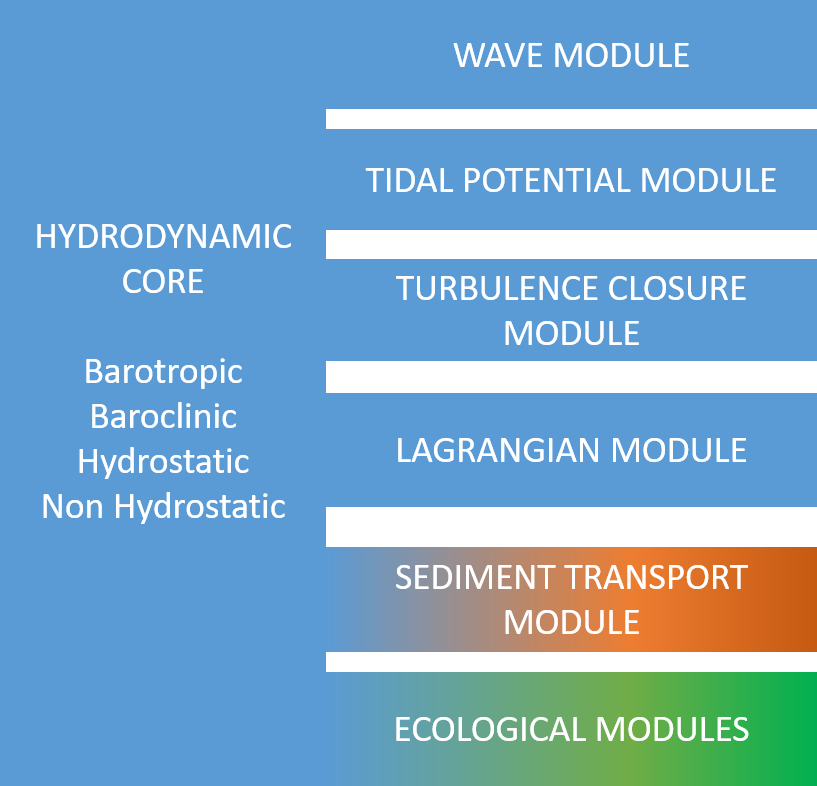
\includegraphics[scale=0.5]{module_scheme.png}
\caption{Model structure and available modules}
\label{module}
\end{figure}

The program uses finite elements for the resolution of
the hydrodynamic equations. These finite elements, together with an
effective semi-implicit time resolution algorithm, makes this program
especially suitable for applications in areas with a complicated geometry
and bathymetry (\Fig \ref{grids}).

\begin{figure}[htbp]
\centering
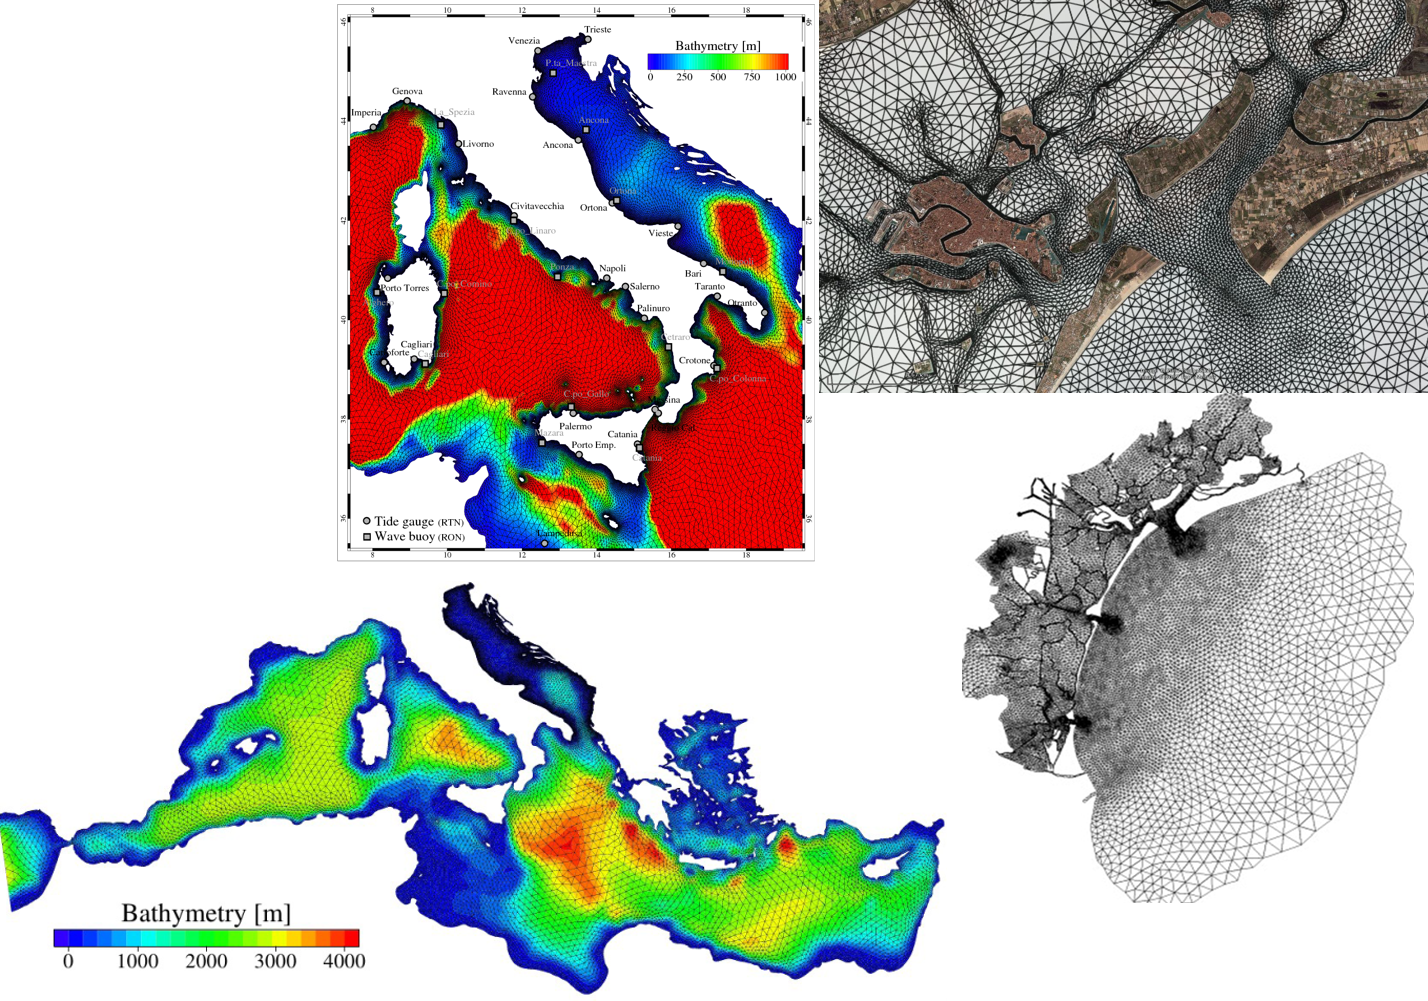
\includegraphics[scale=0.45]{overview_model.png}
\caption{Example modelled domains at different spatial scales, from the Mediterranean Sea to the channels of the Venice Lagoon.}
\label{grids}
\end{figure}


The program \shy{} resolves the depth integrated shallow water equations
and can use both two- or three-dimensional formulations, depending
on the user's needs.

The finite element method has
an advantage over other methods (e.g., finite differences) because it
well adapts to problems dealing with complex
bathymetries and geometries, allowing more flexibility with its subdivision of the system in triangles
varying in form and size.  This flexibility can be used also in situations
where it is not desired to have uniform resolution of the whole basin,
but where a focus in resolution is needed only in some parts of the area.

It is possible to simulate shallow water flats, i.e., tidal marshes
that in a tidal cycle may be underwater during high tide and
dry during ebb tide. This phenomenon is handled by the model
in a mass conserving way, as explained in appendix \ref{mass}.

Finite element methods have been introduced into hydrodynamics since 1973
and have been extensively applied to shallow water equations by numerous
authors \cite{Grotkop73, Taylor75, Herrling77, Herrling78, Holz82}.

% FIXME - new references

The model presented here \cite{Umgies86, Umgies93} uses the mathematical
formulation of the semi-implicit algorithm that decouples the solution
of the water levels and velocity components from each other leading to
smaller systems to solve. Models of this type have been presented from
1971 on by many authors \cite{Kwizak71, Duwe82, Backhaus83}.



	\section{Where and how to get it}
	
%------------------------------------------------------------------------
%
%    Copyright (C) 1985-2020  Georg Umgiesser
%
%    This file is part of SHYFEM.
%
%    SHYFEM is free software: you can redistribute it and/or modify
%    it under the terms of the GNU General Public License as published by
%    the Free Software Foundation, either version 3 of the License, or
%    (at your option) any later version.
%
%    SHYFEM is distributed in the hope that it will be useful,
%    but WITHOUT ANY WARRANTY; without even the implied warranty of
%    MERCHANTABILITY or FITNESS FOR A PARTICULAR PURPOSE. See the
%    GNU General Public License for more details.
%
%    You should have received a copy of the GNU General Public License
%    along with SHYFEM. Please see the file COPYING in the main directory.
%    If not, see <http://www.gnu.org/licenses/>.
%
%    Contributions to this file can be found below in the revision log.
%
%------------------------------------------------------------------------
\label{where} 

\subsection{From website}
From website shyfem.org you can download the latest stable version of the model.
The version released from the website is the stable one and is always updated to the latest release. 
\subsection{From GitHub}

%From |Google Drive| you can
%download the latest and older version of the model. In order to do so, please go to
%|https://drive.google.com/open?id=0B742mznAzyDPbGF2em5NMjZYdHc| and
%download the version you would like to install on your computer. Normally
%this will be the last available version.
Since SHYFEM is a model in constant development, for research purposes the user can download the develop versions, 
and also the latest stable one, from GitHub.


Please go to the |GitHub| website of the \shyfem{} model
|https://github.com/SHYFEM-model/shyfem| and navigate to |releases|.  
You either can visualize the releases or the tags (versions)
of the model and download them. Please see below for the difference
between tags and releases.

If you are a developer then you should install the |git|
versioning system that will give you direct access to the latest versions
of \shyfem{}.  Please see below how to do this.

Here is some information on how the various releases are managed and where to
download the latest version.

There are various types of versions:

\begin{itemize}

\item commit: commits are the smallest changes in the code base. 
Every time changes have been carried out, they will be committed to the repository. 
It is possible to see all the commits of the code
by typing |git-tags| which presents all the commits and also the tags,
which are explained here below.

\item version: the name version is just a shortcut for an existing tag 
or release that will have a version number associated.  
A commit has no version number and can therefore not
be identified in this way.

\item tag: tags are like commits, but a version number is given to
them. This means that these tags are more stable than simple commits. It
is always advisable to download tags in order to be able to easily refer
to the version number of \shyfem{}.

\item release: releases are nothing else than tags, but a name is also
given to this tag. This means that releases should be even more stable
than tags or commits. If you do not need a bleeding edge version, than
these are the versions that you should download.

\end{itemize}

For an easy use of github follow this procedure:
\begin{itemize}
\item to find commits and tags: use |gittags|. Its output provide the latest
 commits and tags (if applied). 

\item to see releases:  go to the github web page
(|https://github.com/SHYFEM-model/shyfem|). Click on |releases| and 
you can directly download the latest
version of \shyfem{}.

 \item to get access to the latest single commits, not available at |github| web page:
\subitem install |git| on your computer. 
\subitem go to the web page and click on |clone| to download the latest version with all
the versioning information included. 
\subitem Unpack the archive in any directory, and enter the newly created directory.
\subitem Type |git fetch| and |git pull| to have the newest commit of the code base.
\end{itemize}

 If you are a developer:
\begin{itemize}
\item you should have git installed on your computer.
\item If you want your changes in code being published do a |pull request| from the |github| website. 
\subitem Please be sure that you base your 
|pull request| on the latest commit (not tag or release). 
\subitem do a |git fetch| and |git pull|
\subitem check if your changes are compatible
\subitem do the |pull request|.
\end{itemize}

 All |pull requests| have to be based on the |develop| branch.




%%%%%%%%%%%%%%%%%%%%%%%%%%%%%%%%%%%%%%%%%%%%%%%%%%%%%%%%%%%%%%%%%%%%%%%%
%%%%%%%%%%%%%%%%%%%%%%%%%%%%%%%%%%%%%%%%%%%%%%%%%%%%%%%%%%%%%%%%%%%%%%%%
%%%%%%%%%%%%%%%%%%%%%%%%%%%%%%%%%%%%%%%%%%%%%%%%%%%%%%%%%%%%%%%%%%%%%%%%

\chapter{Installing SHYFEM}

	\section{Installation}
	
%------------------------------------------------------------------------
%
%    Copyright (C) 1985-2020  Georg Umgiesser
%
%    This file is part of SHYFEM.
%
%    SHYFEM is free software: you can redistribute it and/or modify
%    it under the terms of the GNU General Public License as published by
%    the Free Software Foundation, either version 3 of the License, or
%    (at your option) any later version.
%
%    SHYFEM is distributed in the hope that it will be useful,
%    but WITHOUT ANY WARRANTY; without even the implied warranty of
%    MERCHANTABILITY or FITNESS FOR A PARTICULAR PURPOSE. See the
%    GNU General Public License for more details.
%
%    You should have received a copy of the GNU General Public License
%    along with SHYFEM. Please see the file COPYING in the main directory.
%    If not, see <http://www.gnu.org/licenses/>.
%
%    Contributions to this file can be found below in the revision log.
%
%------------------------------------------------------------------------

The source code of the model is provided in a file named \ttt{\shydist}
or similar, depending on the version of the code. In this case the
version is \version.  The file can be downloaded from the SHYFEM GIT
repository \textcolor{red}{UPDATE LINK TO GIT}\footnote{ https://github.com/shyfemcm/shyfemcm}, or
 in the SHYFEM web-site \textcolor{red}{UPDATE LINK TO WEBSITE} \footnote{http://www.ismar.cnr.it/shyfem/}, as 
described in section \ref{where}.

\subsection{How to choose the right repository for the model}

There is more than one repository for getting the code. Some of the possibilities will be described below.

\begin{enumerate}

\item  the official community repository is https://github.com/shyfemcm/shyfemcm

	This is the official community model repository. Here all official updates and contributions eventually will end up. It might not 	contain the last developments, but it should be stable to be used for all purposes.

	In order to clone this repository, please run:

	git clone https://github.com/SHYFEM-model/shyfem.git

	or download from https://github.com/shyfemcm/shyfemcm

\item  the old pre-community model repository

	https://github.com/SHYFEM-model/shyfem

	This contains the last version pre-community. It is now at
	version 7.5.85 and will not be evolving further

	Please do not use this distribution anymore.

	If for some reasons you still have to use this old version,
	please run:

	git clone https://github.com/SHYFEM-model/shyfem.git

	or download from https://github.com/SHYFEM-model/shyfem

\item  the private ismar community repository

	https://github.com/georgu/shyfemcm-ismar

	Here all the development at the ISMAR institute is going on. The
	repository contains more branches. Depending on what you would
	like to do, once you have downloaded the model you should switch
	to the appropriate branch.

	main		this is the main branch and it should normally
			be the same as the main branch of the official
			repository in point 1 above.

	develop		here all the new developments of ISMAR are being
			kept. If you need a special feature that the
			official branch does not have, please look here.

	feature1	these is a feature branch. Here some new feature
			will be implemented. Once the feature is tested
			it will be ported to the develop branch.

	feature2	etc...

	In order to clone this repository, please run:

	git clone https://github.com/georgu/shyfemcm-ismar.git

	or download from https://github.com/georgu/shyfemcm-ismar

\item  how to update and switch branches

	if you have used the command "git clone" in order to download
	and install the model, you can easily upgrade to a new version
	with this command:

	git pull

	if you get an error, please have a look at the following section
	to resolve the problem.

	To switch branches you do:

	git status		 (this will tell you on what branch you are)
	git checkout develop	(this will switch to the branch develop)

	In order to switch to a different branch, once you have 

\end{enumerate}

\subsection{How to to install the model with git}
In the following there is the description of the list of steps to install from git the model:

\begin{enumerate}
\item  check your repository: refer to previous section.

\item  install git on your computer\\

	run "git --version"\\
	if you see no error, you already have git installed\\
	if not, please install git\\
	with debian, you can run (as superuser)\\
		apt update\\
		apt install git\\

\item  get the latest version of the model:the name of the repository below may change depending on
	your choice on what repository you have chosen to use. Please refer to point 0 above. You have two choices. The first is the preferred one.

	\subitem a) clone directly in your current directory
		git clone  \footnote{https://github.com/shyfemcm/shyfemcm.git} myshyfem
		this will create a directory myshyfem in your current directory
		this directory contains the model code
		be sure not to have an existing myshyfem directory
			in your current directory
		you can give any name to the new shyfem directory
	
	\subitem b) download from Github
		goto  \footnote{https://github.com/shyfemcm/shyfemcm}
		you will see a green button with "Code" written on it
		download the zip file
		do a "unzip -v" to see in what dir the model will be copied
		unzip in a convenient directory
		please remember that with this choice you do not need
		to install git on your computer. However, updating
		the model to a new version means that you will have
		to execute these steps over and over again

\item compile the model

	go into the directory that has been created and run
		make\\
	this should compile the model with standard flags\\
	you can always run "make help" to see other targets\\
	running make check$\_$software will tell you what software is missing for shyfem to be installed
	
\item make a symbolic link: 	
this is not necessary, but useful\\
	goto your home directory and run\\
		ln -s dir-where-shyfem-is-installed shyfem\\
	this will create a link to the new shyfem directory\\
	be sure you do not have a shyfem directory (or link) in your home

\item update the model

	this is needed when new functionality has been added to the model with these commands you can download the latest version easily\\

	updating only works if you have git installed on your computer and you have chosen option 2a above. In case you have chosen 	option 2b you will have to download the model again from scratch.\\

	goto the shyfem directory where the model is installed\\
		git fetch\\
		git pull\\
		make\\

	this will get the latest model version and compile it\\

	if you get an error with "git pull" you probably have changed something in the model code and the pull would overwrite your changes. Save your changes somewhere, then do\\
		git checkout file(s)\\
	where file(s) are the offending file(s)\\
		git pull\\
	and then compare the difference between your files and the new ones\\
\end{enumerate}


Once you have downloaded the model distribution, move the file to
the directory in which you want to install the model and unpack the
distribution. In the following we will assume that the file is in your
home directory and your home directory is called \ttt{\basedir}. However,
any other directory works as well. To unpack the distribution
in your home directory, move there and run the command:

\begin{codem}
    cd \basedir
    tar xzvf \shydist
\end{codem}

At this point a new folder named \ttt{\shydir} has been created. 
This directory is the root of the SHYFEM model. All other commands
given in this chapter assume that you are in this directory. 
Therefore, before reading on, please move into this directory:

\begin{codem}
    cd \shydir
\end{codem}

%%%%%%%%%%%%%%%%%%%%%%%%%%%%%%%%%%%%%%%%%%

\newcommand{\sysfiles}{.bashrc .bash\_profile .profile}

Before compiling it is advisable to install some files for a simpler
usage of the model. As long as you only want to run a simulation, this
step is not strictly necessary. But if you will run some scripts of the
distribution, these scripts will not work properly if you do not install
the model.

In order to install the model, you should run

\begin{code}
    make install
\end{code}

This command will do the following:

\begin{itemize}

\item It hardcodes the installation directory in all scripts of the
model so only programs of the installed version will be executed.

\item It inserts a symbolic link |shyfem| from the home directory to
the root of the SHYFEM installation.

\item It inserts a small snippet of code into the initialization files
\ttt{\sysfiles} that are in your home directory. This will adjust your
path to point to the SHYFEM directory and gives you access to some
administrative commands.

\end{itemize}

After this command you will find the original files that have been changed
in your home directory saved with a trailing number (e.g., |.profile.35624|
or similar).  If you encounter problems, just substitute back these files.

In order to guarantee that your new settings take effect, you have to log
out and log in again.

If you do not want to run the installation routine, you should at least
manually insert a symbolic link to the root of the SHYFEM model and
modify your PATH enviromental variable:

\begin{codem}
    cd
    ln -fs \shydir shyfem
    echo -e "export PATH=$PATH:$HOME/shyfem/fembin" >> .bashrc
\end{codem}

If you have more versions installed, you should use |make install_hard|
in order to use the complete paths of the directories in the scripts.
You can run |make install_hard_reset| to restore the settings previous to
this last installation.

If you want to uninstall the model, you should use the command
|make uninstall|. This will delete the symbolic link, cancel the hard
links in the model scripts and restore the systemfiles \ttt{\sysfiles}
to their original content.

Please note that you still have to delete manually the model
directory. This can be done with the command \ttt{rm -rf \shydir}. 
In this case be aware
that changes done by you to the code will be lost.

For other options please refers to the |Rules.make| file.





	\section{Compilation options and prerequisites}

	
%------------------------------------------------------------------------
%
%    Copyright (C) 1985-2020  Georg Umgiesser
%
%    This file is part of SHYFEM.
%
%    SHYFEM is free software: you can redistribute it and/or modify
%    it under the terms of the GNU General Public License as published by
%    the Free Software Foundation, either version 3 of the License, or
%    (at your option) any later version.
%
%    SHYFEM is distributed in the hope that it will be useful,
%    but WITHOUT ANY WARRANTY; without even the implied warranty of
%    MERCHANTABILITY or FITNESS FOR A PARTICULAR PURPOSE. See the
%    GNU General Public License for more details.
%
%    You should have received a copy of the GNU General Public License
%    along with SHYFEM. Please see the file COPYING in the main directory.
%    If not, see <http://www.gnu.org/licenses/>.
%
%    Contributions to this file can be found below in the revision log.
%
%------------------------------------------------------------------------
% FORMER software.tex

The source code is composed mainly of Fortran 90 files, but files written
in C, Fortran 77, Perl and Shell scripts are also present.

In order to use the model you have to compile it in a Linux Operating
System. Several software products must be present in order to be able
to compile the model. Please refer to the documentation of your Linux
distribution for installing these programs.

\begin{itemize}

\item The package |make| is required for compilation.

\item The |perl| interpreter and the |bash| shell are necessary for compiling.

\item A Fortran 77 and 90 compiler. Supported compilers are the Gnu 
compiler |gfortran|, the Intel Fortran compiler |ifort| and the Portland 
group |pgf90| Fortran compiler.

\item A C compiler. Supported compilers are the Gnu |gcc|, the Intel C
compiler |icc| or the IBM |xlc| C compiler.

\end{itemize}

Please note that you might already have everything available in your
Linux distribution, with the exception maybe of the Fortran compiler.

To find out what software is installed on your computer and what you
still have to install you can run the following command:

\begin{code}
    make check_software
\end{code}

If you get something like |bash: make: command not found|, then you do
not have make installed. Please first install the |make| command and
then run the command again.

The output of the command will show you what software you still have
to install. The |make check_software| is divided into different sections. 
The first section 
concerns the needed software which, if not installed, will not allow you to proceed. 
The next section lists the recommended software, which you really should install,
but that is not necessarily needed for compilation and running. 
The last section lists the optional software (not necessary but it will make your life easier).

You can always run |make check_software| again to check if the software
had been successfully installed. When you are satisfied with the output
you can go to the next section.

Depending on the options that you choose for the compilation you may
need some additional package or library. Usually, the error message
gives you the name of the missing library. The name of the corresponding
package to install can be found at the 
web-page\footnote{https://www.debian.org/distrib/packages} for Debian OS.
Usually, Debian-based (e.g., Ubuntu) distributions have the same name.

Whereas most package names are easy to guess, a common problem refers to
 the developer X11 libraries. In order to be able to compile the
program |grid| you will need to install some packages that may have
different names depending on your distribution. The packages you need to find
 are |libx11-dev|, |x11proto-core-dev| and |libxt-dev|.

Please note that you have to carry out the steps in this section only
the first time you install the model. If you install a new version of
SHYFEM software you can skip these steps.

%%%%%%%%%%%%%%%%%%%%%%%%%%%%%%%%%%%%%%%%%%%
%former compilation.tex 
In order to compile the model you will first have to adjust some settings
in the |Rules.make| file. Assuming that you are already in the SHYFEM
root directory (in our case it would be \ttt{\shydir}), open the file
|Rules.make| with a text editor.  In this file the following options
can be set:

\begin{itemize}

\item |Compiler profile|. Set the level of verbosity of the messages. Use
|SPEED| if you want the maximum performances. Use the other options, in
case of errors, to have more informations.

\item |Compiler|. Set the compiler you want to use. Please see also
the section on needed software and the one on compatibility problems to
learn more about this choice. It is advisable to use the same type of
compiler for C and Fortran.


\item |Parallel compilation|. \textcolor{red}{QUESTA SEZIONE VA TOTALMENTE CONTROLLATA E INTEGRATA}. The code is parallelized either with OpenMP and MPI statements. Here you can set if you want to use it or not.

\textcolor{red}{OMP DA RISCRIVERE}
If you want to run with OMP, you have to change the Rules.make file as follows:

Set the compiler
PARALLEL$\_$OMP=true

Then, in the str file, section para, you have to indicate the number of nodes/cores you want to use for parallel computation, e.g. nomp = 8 means parallel on 8 cores.

If MPI (domain decomposition) is already installed you can skip the part on how to install
gfortran and mpi. Please run make test$\_$mpi from the shyfem base
directory to see if MPI is installed on your computer.

However, you must be sure that also the library METIS is installed. Please
refer to the instructions below.

All examples have been tested on a debian system (Ubuntu) with gfortran. Other linux systems
should be similar, as well as other compilers (Intel).

update the apt system (all commands with apt must be carried out as root): \\
	apt update\\
	apt upgrade\\

\subitem If needed install the gfortran compiler: apt install gfortran. You can check if gfortran is already installed running "gfortran --version".

\subitem If needed install the mpi libraries (openmpi): apt install openmpi. To see if you already have the mpi routines and binaries installed run\\
make test$\_$mpi from the base directory of shyfem.\\

\subitem Install the metis library to create automatic partition of the basin
($http://glaros.dtc.umn.edu/gkhome/metis/metis/overview$). You can install
the system anywhere. Just remember the place, because you will have
to insert this information into the Rules.make file. It is, however,
recommended that you put all the add-on libraries in one place, such as
$HOME/lib$. If you put metis in this directory shyfem will look automatically
for it and you do not have to specify the directory in Rules.make.

\subitem How to compile and run shyfem in MPI mode\\
Change the file Rules.make
	Set the compiler\\
	PARALLEL$\_$MPI = NODE\\ 
	$PARTS = METIS $\\
	$METISDIR = HOME/lib/metis$ or wherever the metis files\\ 
	have been installed. If metis is in $HOME/lib/metis$ you do not have to set this variable.

if METIS is installed in $HOME/lib$ (you should have a directory metis
in this place) you can do everything above by just running

	make rules$\_$mpi\\

recompile:\\

	make cleanall\\
	make fem\\

run shyfem:

	mpirun -np 4 path$\_$to$\_$shyfem/shyfem str-file.str

	test with a different number of domains (above 4 are used)
	if there are errors (there will be...) please let me know



\item |Solver for matrix solution|. There are four different solvers implemented.
The model need to solve a system of matrix equations. In order to do this, four different
solvers are implemented and can be set in the Rules.make file (flag SOLVER).

\subitem 1) The SPARSKIT solver is iterative and quite fast (default);

\subitem 2) The GAUSS solver is a robust direct solver, but quite slow;

\subitem 3) The PARDISO solver is not included in the model code, but can be found in the Intel MKL and linked dynamically during the compilation. This solver is set as a direct solver but can be used also in an iterative mode. 

%\subitem 4) \textcolor{red}{DA ELIMINARE, VECCHIO} The PARALUTION solver works by exploiting both the CPU and the GPU (tested with NVIDIA cards).  This solver should be used with large matrices and with powerful GPUs and is quite fast in these cases. The solver is not included in the model code and, in order to use it, the following steps must be executed:

%    \subsubitem a) In Rules.make set the flags SOLVER (= PARALUTION), PARADIR (solver installation path) and GPU (gpu library);

%    \subsubitem b) Execute  the following command to download and compile the PARALUTION library

%\begin{center}
%\begin{tabular}{ l p{7cm} }
%|make para_get && make para_compile| 
%\end{tabular}
%\end{center}

%    \subsubitem c) Proceed with the normal compilation of SHYFEM.

%It is recommended to use the OpenCL or CUDA gpu libraries, which however require the installation of some system packages. For more information see the README file in the directory fempara/.

\subitem 4) The PETSC solver, required if you run in parallel with MPI. Before you run shyfem with PETSC please be sure that shyfem runs smoothly in MPI mode. Refer to appencix for installation and use.


 
%|SPARSKIT| is an iterative solver, 
%quite fast, and is the default option. The |GAUSS| solver is a robust direct solver, but it is quite slow. 
%|PARDISO| is set as direct solver but can be used as iterative solver as well. 
%It can be fast, but it is not included in the code, since it is not provided with 
%a compatible license. In order to use it, you need an external library (dynamically linked) 
%provided with the Intel MKL.

%Finally, the |PARALUTION| solver works by exploiting both the CPU and the GPU 
%(tested with NVIDIA cards).
 %If you have a powerful graphics card and/or if you use computational grids with 
%many elements (large matrices), this solver should be the fastest. To use it you
 %need to set some variables in the Rules.make file. 
%The folder where the solver code will be downloaded (|PARADIR|), the graphical libraries 
%used in the compilation (GPU) and the use of OMP compilation (|PARALLEL_OMP|). 
%It is recommended to use the OpenCL or CUDA libraries, which however require the 
%installation of some system packages. At this point 
%it is necessary to execute the command |make para_get && make para_compile|


If the compilation is successful, you can execute |make fem|.

\item |NetCDF library|. If you want output files in NetCDF format
you need the NetCDF library. Normally netcdf should already be installed. To enable netcdf you
must set in Rules.make the following:

NETCDF = true

If the directory where netcdf is not installed you have to give it
explicitly in NETCDFDIR.


\item |GOTM library|. The GOTM turbulence model (version 4.0.0) is already included in
the code. However, a newer and better tested version is available as an
external module. In order to use it please let this variable to true. This
is the recommended choice. You will need a Fortran 90 compiler to enable
this choice.

\item |Ecological module|. This option allows for the inclusion of an
ecological module into the code. Choices are between |EUTRO|
and |AQUABC|. Please refer to information given in Section \ref{eco}
to run these programs.

%\item |Fluid mud|. 
%\textcolor{red}{ADD EXPLANATION}

%This is an experimental feature. Don't use it
%if you are not a developer.

\end{itemize}

Once you have set all these options you can start compilation with

\begin{code}
    make clean
    make fem
\end{code}

This should compile everything. In the case of a compilation error,
 messages will be shown both while the program is compiling as 
well as at the bottom of the output (where a check occurs to see if 
the main routines have been compiled).

Please remember that you will always have to run the commands above
when you change settings in the |Rules.make| file. If you only change
something in the code, or if you only change dimension parameters, it
might be enough to run only |make fem|, which only compiles the necessary
files. However, if you are in doubt, it is always a good idea to run
|make clean| or |make cleanall| before compiling, in order to start from
a clean state.
%%%%%%%%%%%%%%%%%%%%%%%%%%%%%%%%%%%%%%%
%former summary_installing.tex 

A summary of administrative commands available in SHYFEM is given below: \vspace{0.5cm}

\begin{center}
\begin{tabular}{ l p{7cm} }
|make version|		&	shows version of distribution \\
|make clean|		&	deletes objects and executables from a previous
                        	compilation \\
|make cleanall|		&	same as |make clean| but also deletes 
				compiled libraries \\
|make fem|		&	compiles SHYFEM \\
|make doc|		&	makes this manual (|femdoc/shyfem.pdf|) \\
|make check_software|	&	checks the availability of installed software \\
|make check_compilation|&	checks if all programs have been compiled \\
|make changed|		&	finds files that are changed with respect to the
				original distribution \\
|make changed_zip|	&	zips files that are changed with respect to the
				original distribution to the file 
				|changed_zip.zip| \\
|make install|		&	installs SHYFEM \\
|make uninstall|	&	uninstalls SHYFEM \\
\end{tabular}
\end{center}

\vspace{0.5cm}
Finally, if you have installed the model with |make install|, 
the following utility commands are available \vspace{0.5cm}

\begin{center}
\begin{tabular}{ l l }
|shyfemdir|		&	shows information about actual SHYFEM
				settings \\
|shyfemdir fem_dir|	&	sets |fem_dir| to be the new default 
				SHYFEM version \\
|shyfeminstall|		&	shows information about original SHYFEM 
				installation \\
|shyfemcd|		&	moves into root of actual SHYFEM directory \\
\end{tabular}
\end{center}





	\section{Compatibility problems}
	
%------------------------------------------------------------------------
%
%    Copyright (C) 1985-2020  Georg Umgiesser
%
%    This file is part of SHYFEM.
%
%    SHYFEM is free software: you can redistribute it and/or modify
%    it under the terms of the GNU General Public License as published by
%    the Free Software Foundation, either version 3 of the License, or
%    (at your option) any later version.
%
%    SHYFEM is distributed in the hope that it will be useful,
%    but WITHOUT ANY WARRANTY; without even the implied warranty of
%    MERCHANTABILITY or FITNESS FOR A PARTICULAR PURPOSE. See the
%    GNU General Public License for more details.
%
%    You should have received a copy of the GNU General Public License
%    along with SHYFEM. Please see the file COPYING in the main directory.
%    If not, see <http://www.gnu.org/licenses/>.
%
%    Contributions to this file can be found below in the revision log.
%
%------------------------------------------------------------------------

The SHYFEM program is designed to work with most of the compilers
that are available. Normally there should be no problems with
compatibility. However you have to keep in mind some points that are
listed below.

\begin{itemize}

\item With |ifort| it is possible to open the same file in
read only mode more than once. This is useful, e.g., if you have two
open boundaries, but you want to prescribe the same value on these
two boundaries. With |gfortran| or |pgf90| you cannot do this. A file,
even in read only mode, can be opened only once. In the above example
you therefore have to copy the input file to a new name (duplicate it)
and then prescribe the two different files as boundary conditions.

\item With |gfortran| it is very difficult to decide if a file is
formatted or unformatted. Some modules allow the use of either formatted
or unformatted input files, where the check on the file type is made
via software. In case of |gfortran| this may not work reliably. The only
solution to this problem is to specify the file type directly in the code.

\item Objects generated during compilation and libraries used in linking
are normally not compatible between compilers. It implies that when you
 switch compiler, you will have to recompile everything with
|make cleanall; make fem|. Otherwise you will encounter errors during
the linkage process.

\item Unformatted files are normally not portable between different
compilers. You normally cannot use a basin file created with programs
compiled with one compiler together with a program compiled with another
compiler. The same is true for unformatted data files (initial conditions,
wind and meteo forcing, etc.).

If you have problems reading a basin file, please use |shybas|, functionalities discussed in appendix \ref{postproc_prg}.
If this is
not working chances are high that you have the problem described above.
In case of unformatted data files the diagnosis is not so easy. In any
case, you can solve the problem recompiling all programs with the commands
|make cleanall; make fem| and then re-creating all unformatted files
with the newly compiled programs. In case of the basin file, you will
have to run the pre-processor on the grid again.

If you have obtained unformatted data files from others, then there is
really no easy solution to this problem. Exchanging unformatted files
between different computers and compilers is never a good idea.

\item A similar problem exists if you switch files between different
architectures (32 bit and 64 bits), even if created with the same
compiler. These files are normally not portable.

\item Nan values (Not a Number) are treated differently between different
compilers. Nan values are created if a not well defined operation is
executed (divide by 0 or square root of a negative number). All compilers
above (except |pgf90|) treat Nans to be not comparable to any number.
This means that a logical expression |a.eq.a| is always false if |a|
is a Nan. However the |pgf90| compiler treats Nans to be comparable
to any other number. So, an expression like |a.ne.a| will evaluate to
true. SHYFEM includes code to handle these problems gracefully, but
incompatibilities might still show up.

\item In parallel execution you might get a segmentation fault, 
if the program attempts to access a memory location that it is not allowed to access, 
or attempts to access unproperly a memory location, during
execution. This is normally due to limited stack size. You can change
the behavior by increasing the stack size (|ulimit -s unlimited|)
on the console before running the program. Compilers may behave
differently. Please see also the section on parallel execution in the
file |Rules.make|.

\end{itemize}








%%%%%%%%%%%%%%%%%%%%%%%%%%%%%%%%%%%%%%%%%%%%%%%%%%%%%%%%%%%%%%%%%%%%%%%%
%%%%%%%%%%%%%%%%%%%%%%%%%%%%%%%%%%%%%%%%%%%%%%%%%%%%%%%%%%%%%%%%%%%%%%%%
%%%%%%%%%%%%%%%%%%%%%%%%%%%%%%%%%%%%%%%%%%%%%%%%%%%%%%%%%%%%%%%%%%%%%%%%

\chapter{Preprocessing: The numerical grid}

	\section{Overview}
	
%------------------------------------------------------------------------
%
%    Copyright (C) 1985-2020  Georg Umgiesser
%
%    This file is part of SHYFEM.
%
%    SHYFEM is free software: you can redistribute it and/or modify
%    it under the terms of the GNU General Public License as published by
%    the Free Software Foundation, either version 3 of the License, or
%    (at your option) any later version.
%
%    SHYFEM is distributed in the hope that it will be useful,
%    but WITHOUT ANY WARRANTY; without even the implied warranty of
%    MERCHANTABILITY or FITNESS FOR A PARTICULAR PURPOSE. See the
%    GNU General Public License for more details.
%
%    You should have received a copy of the GNU General Public License
%    along with SHYFEM. Please see the file COPYING in the main directory.
%    If not, see <http://www.gnu.org/licenses/>.
%
%    Contributions to this file can be found below in the revision log.
%
%------------------------------------------------------------------------
\label{preprocessing}

Before you can start using the model you have to create a numerical grid.
Creating a grid is more difficult for models that work on unstructured grids
(like finite element models) than for finite difference models, where
often it is enough to have a regular gridded bathymetry to start running
simulations.

\begin{figure}[htbp]
\centering
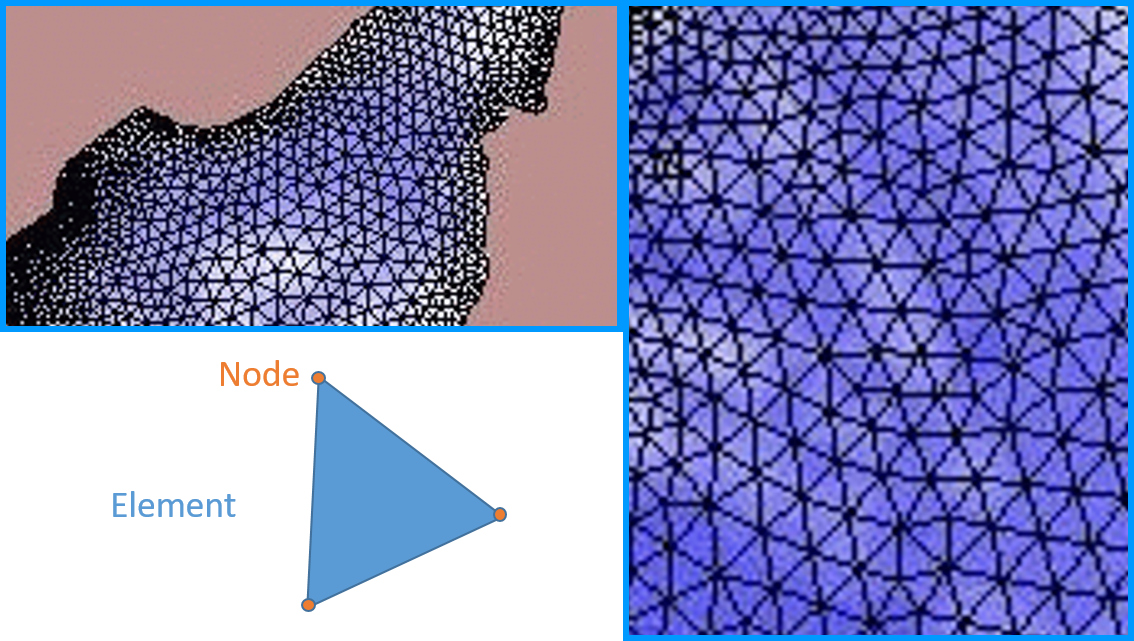
\includegraphics[scale=0.5]{example_finite_elements.png}
\caption{Example of  a finite element grid. Zoom on elements. Vertices are called nodes.}
\label{grd_example}
\end{figure}

the SHYFEM finite element grids are composed of triangular elements, 
where the vertices are called nodes. For a thorough description of the 
approach used with staggered finite elements
over such a grid refer to Appendix A.2.

This chapter describes the steps needed to create a numerical grid for SHYFEM.

The files containing the informations on the computational grid, used by SHYFEM, are two:

\begin{itemize}
\item |filename.grd| formatted
\item |filename.bas| unformatted
\end{itemize}

You must create the first one, while the second can be obtained automatically by
the first. The |bas| file is the one really used by the model.

The |grd| file can be composed of 3 different parts, describing different geometric
objects, which are: Nodes, Elements, Lines. These parts are the following:

\begin{itemize}
\item Node section, containing the nodes information and coordinates
\item Element section, containing the elements information and the their nodes
\item Line section, containing the domain contour infomation and nodes
\end{itemize}

The presence of these structures depends on type of |grd| file, for example,
in a boundary line the structures will be the line and its nodes.
For more details on the format, please, refer to |grd| file appendix~\ref{grid}.

The steps to create a |grd| file are the following and they will be described below:

\begin{enumerate}

\item obtain raw digital data of the coastline and the bathymetry and
  convert them into a |grd| format

\item smooth and reduce the coastline if needed

\item create the numerical grid with a mesh generator

\item regularize the grid

\item interpolate bathymetry onto the created grid

\item create the unformatted |bas| file

\end{enumerate}

These steps are described in the following sections.


	\section{Coastline and bathymetry}
	
%------------------------------------------------------------------------
%
%    Copyright (C) 1985-2020  Georg Umgiesser
%
%    This file is part of SHYFEM.
%
%    SHYFEM is free software: you can redistribute it and/or modify
%    it under the terms of the GNU General Public License as published by
%    the Free Software Foundation, either version 3 of the License, or
%    (at your option) any later version.
%
%    SHYFEM is distributed in the hope that it will be useful,
%    but WITHOUT ANY WARRANTY; without even the implied warranty of
%    MERCHANTABILITY or FITNESS FOR A PARTICULAR PURPOSE. See the
%    GNU General Public License for more details.
%
%    You should have received a copy of the GNU General Public License
%    along with SHYFEM. Please see the file COPYING in the main directory.
%    If not, see <http://www.gnu.org/licenses/>.
%
%    Contributions to this file can be found below in the revision log.
%
%------------------------------------------------------------------------

In order to create the computational grid you need data of the coast line
and of the bathymetry.
First of all you must create a coast line in |grd| format. You can do
this with your own tools, but you could find useful the script
|coast.pl|, which converts a simple coast file (x,y) into a |grd| file.
To use it run:

\begin{code}
    coast.pl mpcoast.dat > coast.grd
\end{code}

After this step you can check your cost line with the |grid| program:

\begin{code}
    grid coast.grd
\end{code}

Likewise, if you have a bathymetry in a simple (x,y,z) format, you can
convert it with:

\begin{code}
    bathy.pl mpbathy.dat > depth.grd
\end{code}

You can check the file |depth.grd| with |grid| as well. However, this file 
will be used only after the creation of the mesh.

Please note that UTM coordinates are normally huge numbers, there
might be an accuracy problem when you try to create the grid. If this
happens, you should first shift your UTM coordinates so that the origin
of your new coordinate system coincides with the central point of your
grid. This translation can be done using the program |grd_transl.pl|.

Other transformation routines are:

\begin{itemize}

\item |dxf2grd.pl|  Transforms a grid from |dxf| (Autocad) to |grd|
format. This is still experimental.

\item |kml2grd.pl|  Transforms a grid from the Google Earth format |kml|
to |grd| format.

\item |xyz2grd.pl|  Transforms a simple list of nodes to |grd|
format. Every line contains 3 values $(x,y,z)$ or two values $(x,y)$,
when the information on depth is missing.

\end{itemize}

Please note that for SHYFEM depth values have to be positive. If your
files have depth values as negative numbers, you will have to invert
them. You can use the command

\begin{code}
    grd_modify.pl -depth_invert grd-file
\end{code}

to achieve this task.



	\section{Boundary line: smoothing and reducing}
	
%------------------------------------------------------------------------
%
%    Copyright (C) 1985-2020  Georg Umgiesser
%
%    This file is part of SHYFEM.
%
%    SHYFEM is free software: you can redistribute it and/or modify
%    it under the terms of the GNU General Public License as published by
%    the Free Software Foundation, either version 3 of the License, or
%    (at your option) any later version.
%
%    SHYFEM is distributed in the hope that it will be useful,
%    but WITHOUT ANY WARRANTY; without even the implied warranty of
%    MERCHANTABILITY or FITNESS FOR A PARTICULAR PURPOSE. See the
%    GNU General Public License for more details.
%
%    You should have received a copy of the GNU General Public License
%    along with SHYFEM. Please see the file COPYING in the main directory.
%    If not, see <http://www.gnu.org/licenses/>.
%
%    Contributions to this file can be found below in the revision log.
%
%------------------------------------------------------------------------

Every |grd| file can be open with the |grid| program.
Normally, the coastline needs some post-processing.
It might either have resolution which is too high, island
might show up as open lines etc..

It is important that there is one closed boundary line that
defines the whole domain of the computation. If you have an
open coastline, please close the line with the routine |grid|
at the places where you want your open boundary to be.

Once this domain boundary line has been defined, care has
to be taken that the lines inside this domain, which denote
islands, are closed.

Finally, the resolution of the boundary lines (coast and islands)
have to be adjusted if you use the meshing program here provided. 
If the coastline is left as it is you might
have a much too high resolution along the boundaries. This is due
to the fact that the meshing algorithm does not discard any points
given to it. This means that all boundary nodes are used for the meshing.
Therefore, if you have a very high resolution boundary line, you will
get many elements along the boundary and relatively little elements
(depending on the number of internal points) in the inside of the
basin.

Smoothing and reduction of the boundary lines can be done with the
routine |reduce|. The command is

\begin{code}
    reduce -s sigma -r reduct coast.grd
\end{code}

Here |sigma| specifies the length scale for the smoothing operator
and |reduct| is the length scale below which points may be deleted.
Both values have to be given in the same units of the coordinates
of the file |coast.grd|, so normally meters.
The smoothed file can be found in |smooth.grd| and the subsequently
reduced file in |reduct.grd|. 

If there are some points in the boundary line that should not be smoothed
they can be given a depth value of -1. This is a flag that indicates
that the position of these points will not be touched.




	\section{Manipulating nodes, lines and elements: the grid program}
	
%------------------------------------------------------------------------
%
%    Copyright (C) 1985-2020  Georg Umgiesser
%
%    This file is part of SHYFEM.
%
%    SHYFEM is free software: you can redistribute it and/or modify
%    it under the terms of the GNU General Public License as published by
%    the Free Software Foundation, either version 3 of the License, or
%    (at your option) any later version.
%
%    SHYFEM is distributed in the hope that it will be useful,
%    but WITHOUT ANY WARRANTY; without even the implied warranty of
%    MERCHANTABILITY or FITNESS FOR A PARTICULAR PURPOSE. See the
%    GNU General Public License for more details.
%
%    You should have received a copy of the GNU General Public License
%    along with SHYFEM. Please see the file COPYING in the main directory.
%    If not, see <http://www.gnu.org/licenses/>.
%
%    Contributions to this file can be found below in the revision log.
%
%------------------------------------------------------------------------

The |grid| program allows one not only to visualize 
the |grd| files but provides also a graphical user interface 
to manipulate the different items of the grid (Nodes, Elements, Lines).
The command line and the options available for this program are following reported.

\begin{verbatim}
grid [-options] [files] 

Options :
  -o   do not outline elements      -f   fill elements with color     
  -k   do extra checking            -u   check if nodes are used      
  -T   show type instead of depth   -c#  use color table #            
  -h   print this help screen       -a   ask for file names           
  -d   display  (only X11)          -g   geometry (only X11)          
  -M#  scale color to depth #       -S#  size of color table is #     
  -N#  scale factor for nodes is #  -V#  scale factor for vectors is #
  -C   color nodes and lines        -On  use n as output file name    
  -t#  use type # for new items
\end{verbatim}

\textbf{General GUI commands}

\descrpn{|scroll|}
\descrptext{%
zoom in and out
}
\par
\descrpn{|right click|}
\descrptext{%
select item
}
\par
\descrpn{|left click|}
\descrptext{%
confirm item
}
\par
\descrpn{|up arrow|}
\descrptext{%
increase the node size
}
\par
\descrpn{|down arrow|}
\descrptext{%
decrease the node size
}
\par

The main GUI menu is composed of

\descrpn{|File|}\par
\descrpn{|View|}\par
\descrpn{|Show|}\par
\descrpn{|Node|}\par
\descrpn{|Element|}\par
\descrpn{|Line|}\par
\descrpn{|Change|}\par

\textbf{File menu}

\descrpn{|Cancel|}
\descrptext{%
Obsolete command
}
\par
\descrpn{|Refresh|}
\descrptext{%
Refresh the screen view (to be done to view the last change to the grid)
}
\par
\descrpn{|Print|}
\descrptext{%
Create a Black and White PostScript of the grid |plot.ps|
}
\par
\descrpn{|Save|}
\descrptext{%
Save changes in |save.grd|
}
\par
\descrpn{|Exit|}
\descrptext{%
Quit GRID program
}
\par

\textbf{View menu}

\descrpn{|Zoom Window|}
\descrptext{%
Zoom in a delimited window defined by left clicking two points (left-bottom and right-top)  
}
\par
\descrpn{|Zoom in|}
\descrptext{%
Obsolete command replaced by mouse scroll
}
\par
\descrpn{|Zoom out|}\descrptext{%
Obsolete command replaced by mouse scroll
}
\par
\descrpn{|Total View|}
\descrptext{%
Go back to the total view of the grid
}
\par
\descrpn{|Move|}
\descrptext{%
Obsolete command
}
\par

\textbf{Show menu}

\descrpn{|Show Node|}
\descrptext{%
All the items selected by right clicking will be nodes
}
\par
\descrpn{|Show Element|}
\descrptext{%
All the items selected by right clicking will be elements
}
\par
\descrpn{|Show Line|}
\descrptext{%
All the items selected by right clicking will be lines
}
\par

\textbf{Node menu}

\descrpn{|Make Node|}
\descrptext{%
Create a new node by left clicking
}
\par
\descrpn{|Del Node|}
\descrptext{%
Delete a node by selecting it (right click) and confirming it (left click). |Refresh| to see the changes.
}
\par
\descrpn{|Move Node|}
\descrptext{%
Move a node in a new position. 
Select it (right click) and confirm it (left click), give the new position (left click). |Refresh| to see the changes.
}
\par
\descrpn{|Unify Node|}
\descrptext{%
Unify two different nodes. 
Select the first node you want to unify (right click) and confirm it (left click), select the second node (left click). |Refresh| to see the changes.
}
\par

\textbf{Element menu}

\descrpn{|Make Element|}
\descrptext{%
Create a new element.
Create new nodes (left click) or select and confirm (right-left click) each node of the new element, clicking twice on the last one to close the element. The element has to be created in anti-clockwise sense.
}
\par
\descrpn{|Del Element|}
Remove the element but not its nodes.
\descrptext{%

}
\par
\descrpn{|Remove Element|}
Remove the element and its nodes.
\descrptext{%

}
\par

\textbf{Line menu}

\descrpn{|Make Line|}
\descrptext{%
Create a new line.
Create new nodes (left click) or select and confirm (right-left click) each node of the new line, clicking twice on the last one. In case of a close line it has to be created in anti-clockwise sense.
}
\par
\descrpn{|Del Line|}
\descrptext{%
Remove the line but not its nodes.
}
\par
\descrpn{|Remove Line|}
\descrptext{%
Remove the line and its nodes.
}
\par
\descrpn{|Split Line|}
\descrptext{%
Split the line in two parts.
}
\par
\descrpn{|Join Line|}
\descrptext{%
Join two lines in one.
}
\par
\descrpn{|Del Node|}
\descrptext{%
Delete the node from line but not from the domain.
}
\par
\descrpn{|Remove Node|}
\descrptext{%
Remove the node from line.
}
\par
\descrpn{|Insert Node|}
\descrptext{%
Insert a new node on the line.
}
\par

\textbf{Change menu}

\descrpn{|Change Depth|}
\descrptext{%
Change the depth of the selected item.
}
\par
\descrpn{|Change Type|}
\descrptext{%
Change the type of the selected item.
}
\par








	\section{Creating the mesh}
	
%------------------------------------------------------------------------
%
%    Copyright (C) 1985-2020  Georg Umgiesser
%
%    This file is part of SHYFEM.
%
%    SHYFEM is free software: you can redistribute it and/or modify
%    it under the terms of the GNU General Public License as published by
%    the Free Software Foundation, either version 3 of the License, or
%    (at your option) any later version.
%
%    SHYFEM is distributed in the hope that it will be useful,
%    but WITHOUT ANY WARRANTY; without even the implied warranty of
%    MERCHANTABILITY or FITNESS FOR A PARTICULAR PURPOSE. See the
%    GNU General Public License for more details.
%
%    You should have received a copy of the GNU General Public License
%    along with SHYFEM. Please see the file COPYING in the main directory.
%    If not, see <http://www.gnu.org/licenses/>.
%
%    Contributions to this file can be found below in the revision log.
%
%------------------------------------------------------------------------

In order to create a very good quality mesh, it is advisable to use a dedicated program. Two different open-source options are here recommended:
\begin{itemize}
\item GMSH (https://gmsh.info/)
\item JIGSAW (https://github.com/dengwirda/jigsaw)
\end{itemize}

GMSH is a fast and user-friendly meshing tool with parametric input and advanced visualization capabilities,
normally available in most of the Linux distributions. The specification of any input is done either interactively using the graphical user interface, in ASCII text |.geo| format, or using the C++, C, Python or Julia Application Programming Interface (API). GMSH allows to produce high-quality mesh also by not advanced users, thanks to the interactive interface and intuitive menu. Once the mesh has been produced and exported as |.msh| file, this can be converted in SHYFEM |.grd |.

The following routines, provided with SHYFEM source code, convert the format of the files:

\begin{itemize}
     \item |grd2gmsh.pl| Converts a |grd| format coast line in a |geo| format file,
           readable from |gmsh|. You have to create Plain Surface with 
           |gmsh| gui. Place them before the Size Filed and add manually 
           Physical Surface.
     \item |gmsh2grd.pl| Converts a |msh| (gmsh format) mesh in a |grd| mesh. Check the
           generated mesh with the command grid -k gsmh\_msh.grd for
           clockwise elements and node connections.
\end{itemize}


JIGSAW(GEO) is designed to produce Delaunay triangulations and Voronoi tessellations appropriate for unstructured finite-volume/element type models. Grids can be generated in local two-dimensional domains or over general spheroidal surfaces. Mesh resolution can be adapted to follow complex and detailed user-defined metrics, including topographic contours and coastal features. In addition to the C++ source code, MATLAB/OCTAVE and Python based scripting interfaces are available, offering facilities for file I/O, mesh visualization and pre-/post-processing. JIGSAW includes both algorithms for the construction of new meshes, as well as optimization-driven methods for the improvement of existing grids. The output mesh could be saved both in |.vtk| and |.msh| formats. JIGSAW is mainly oriented to advanced users handling by scripting the generation of meshes with a massive amount of elements.


If you want to use the meshing algorithm provided with the |SHYFEM| package,
called |mesh|, see |mesh -h| for help of the command line options. 

In order to use the |mesh| algorithm you will have to provide to the program
a coastline in which the program will insert triangles. There are some
things to remember:
\begin{itemize}
    \item There must be exactly one closed outer (external) line that will enclose
all the other lines given in the coastline file. This means that it is
not possible to mesh two independent domains at the same time. Clearly,
you can divide the grid file into more files, each of which contains
just one independent domain. These files can then be meshed independently.

    \item The program normally is able to find out what is the external line. It
will simply be the line that encloses all the other lines. If no such line
is found, then this will lead to an error. The program will distinguish
between the external line, islands and fault lines. Fault lines are lines
that will constrain triangles to not cross these lines. For example,
putting a fault line along the edge of a channel will ensure that the
triangles will not cross the channel edge but will be placed along
this edge.
\end{itemize}

In order to decide what line is of which type, the program considers the
largest closest line as the external line, all other lines as islands, and
any open line as a fault line. Normally this is the expected behavior. The
program will classify these lines only if the line type is 0.

If you want to overwrite this behavior you can give explicit line types to the lines in the coast line file:
\begin{itemize}
    \item     type 1 signals an external line
    \item  type 2 signals an island
    \item  type 4 signals a fault line
\end{itemize}

Clearly there can
be only one line with type 1. If you have more than one line with type
1 the program will exit with an error. You can however have a fault line
which is closed, a behavior that will not be possible with the automatic
determination of line types, because a closed line with type 0 is always
an island. Clearly an open line with type 2 (island) is also an error.


The |mesh| routine is able to create a grid with uniform or  
different resolution mesh, depending on user interest.

\begin{verbatim}
MESH - Automatic Grid Generation Routine - Version 1.75 
       1995-2009 (c) Georg Umgiesser - ISMAR-CNR        

Options :
 -b   do not refine boundaries      -n   do not insert internal nodes
 -s#  passes for smoothing          -o#  relax. par. for smoothing   
 -I#  number of internal nodes      -B#  number of boundary nodes    
 -R#  overall resolution            -a#  obtain this aspect ratio    
 -g#  element type for background   -h   show this help screen  
\end{verbatim}


If you want a grid with a uniform solution all over, then
you are already in a position to run the meshing algorithm.
You just say: |mesh -I2000 coast-new.grd| and then
the constructed mesh will be in final.grd. The number 2000
means that you want aprox. 2000 internal points in the domain.
You may adjust this number to your needs.

However, you will normally want to have different resolution
in the domain (high at the inlets of lagoons, at interesting
sites like harbours etc..). Then you have to construct a
background grid that gives an indication to the meshing
algorithm what kind of resolution is needed in what area.

You open the coastline with grid and construct elements
that cover the parts or all of the domain. The areas where
no background grid exists will use the (constant) resolution of the
domain computed by the routine mesh using the total number of
internal nodes (2000 in this example).

Where a background grid exists the model uses the depth values at the
element vertices (nodes) to compute a new value for this resolution.
The depth value acts like a factor that multiplies the constant
overall resolution to obtain a local resolution. So, for example,
constructing a background grid and setting all depth values to 1
would not change the resolution at all from a situation without
background grid. A factor higher than 1 increases the resolution
and one smaller than 1 decreses it. Therefore, in areas where
resolution should be higher than average you can set it to
2 or higher, and in other areas, where you want lower resolution,
you can set it to 0.5 or lower. All nodes of the background grid
need to have a depth (resolution) value. Inside each background
element the resolution is interpolated between the three nodes
(vertices).

In order to distinguish the background grid from the elements
that are constructed by the meshing routine, they must become
a unique element type. You can set it to a value that is not
used for other elements (99 is a good choice). All elements
of the background grid must have this element type.

Extract the background grid from the grid file you just
have constructed by running exgrd (fully described in Appendix \ref{postproc_prg}): "exgrd -LS coast-new.grd".
The file "new.grd" contains only the background grid. Rename it to
something more useful (mv new.grd bck1.grd).
The following is a recapitulation of steps for the background grid creation:

\begin{itemize}
\item        manually construct background grid using coast-new.grd
\item        delete coastline (|exgrd -LS coast-new.grd|).
		This leaves only background elements in file.
\item        set depth at nodes for resolution
\item        set type in elements to 99 
\item        rename to bck1.grd using command:   mv new.grd bck1.grd
\end{itemize}

Now you are ready to start the meshing algorithm.

\subsection{Meshing of the basin}

The main options of mesh routine are:

\begin{verbatim}
        -I2000          use aprox. 2000 internal nodes for the domain
        -g99            element type of background grid is 99
\end{verbatim}

With this parameters the call to mesh would be:

\begin{verbatim}
        mesh -I2000 -g99 coast-new bck1
\end{verbatim}

The created mesh can be found in final.grd.

Please note that you can specify more than one file for the coast line,
so you could keep the domain line and the island lines in seperate files.
You can also have different background grid for different areas in
different files. So a call like this is also possible:

\begin{verbatim}
        mesh -I2000 -g99 coast island1 island2 bck1 bck2 bck3
\end{verbatim}

After the meshing please have a look at the result (final.grd).
If you need more overall resolution, increase the number of internal
points (here 2000). If you need more resolution in the background grid,
open the background file and increase the factor (depth) value where needed.
You might also need other areas with a background grid. Once you
are satisfied with the result please save it to a more meaningful name.

\begin{verbatim}
        mesh -I2000 -g99 coast-new bck1
        mv final.grd mesh1.grd
\end{verbatim}

\subsection{Adjust elements for regularity}

After the creation of the mesh, the grid is still not good enough
for usage in a finite element model. This is due to the fact that
the grid is too irregular. Therefore a program has to be applied
that regularizes the grid.

The program is called |regularize|. It must be given the input grid file
(irregular) and creates a new one with much more regular characteristics.
The program has to be called as:

\begin{verbatim}
        regularize mesh1.grd mesh2.grd
\end{verbatim}

In this case the new regular grid is in |mesh2.grd|. Note that you
can use this program even if you have made your grid using a program
different from |mesh|.



	\section{Interpolating the bathymetry into the grd file}
	
%------------------------------------------------------------------------
%
%    Copyright (C) 1985-2020  Georg Umgiesser
%
%    This file is part of SHYFEM.
%
%    SHYFEM is free software: you can redistribute it and/or modify
%    it under the terms of the GNU General Public License as published by
%    the Free Software Foundation, either version 3 of the License, or
%    (at your option) any later version.
%
%    SHYFEM is distributed in the hope that it will be useful,
%    but WITHOUT ANY WARRANTY; without even the implied warranty of
%    MERCHANTABILITY or FITNESS FOR A PARTICULAR PURPOSE. See the
%    GNU General Public License for more details.
%
%    You should have received a copy of the GNU General Public License
%    along with SHYFEM. Please see the file COPYING in the main directory.
%    If not, see <http://www.gnu.org/licenses/>.
%
%    Contributions to this file can be found below in the revision log.
%
%------------------------------------------------------------------------

After the grid creation, with |mesh| or other programs, you must interpolate the
bathymetry.
The bathymetry must be contained in a |grd| file, previously created.
This file, together with the basin onto which the bathymetry has to be 
interpolated (e.g. mesh2.grd, example below), has to be specified for the program |shybas|, fully 
described in Appendix \ref{elab_grd}.
The simplest call is: 

\begin{verbatim}
        shybas -bfile bathy.grd mesh2.grd
\end{verbatim}

where |bathy.grd| is the |grd| file with the bathymetry values and
|mesh2.grd| is the basin for which to interpolate the bathymetry.
Different types of interpolation can be used. Please run
|shybas -h| for more options.


%\subsection{Create basin for FEM model (bandwidth optimization)}

%Before proceeding to the simulations we must first create a
%representation of the basin suitable for the finite element model.
%
%In order to create the finite element reppresentation of the
%grid, please run "vpgrd mesh3". This creates a file mesh3.bas.
%This is a binary file suitable for being read by the finite
%element model.\\

%        vpgrd mesh3\\



	\section{Creating the bas file}
	
%------------------------------------------------------------------------
%
%    Copyright (C) 1985-2020  Georg Umgiesser
%
%    This file is part of SHYFEM.
%
%    SHYFEM is free software: you can redistribute it and/or modify
%    it under the terms of the GNU General Public License as published by
%    the Free Software Foundation, either version 3 of the License, or
%    (at your option) any later version.
%
%    SHYFEM is distributed in the hope that it will be useful,
%    but WITHOUT ANY WARRANTY; without even the implied warranty of
%    MERCHANTABILITY or FITNESS FOR A PARTICULAR PURPOSE. See the
%    GNU General Public License for more details.
%
%    You should have received a copy of the GNU General Public License
%    along with SHYFEM. Please see the file COPYING in the main directory.
%    If not, see <http://www.gnu.org/licenses/>.
%
%    Contributions to this file can be found below in the revision log.
%
%------------------------------------------------------------------------

The pre-processing routine |shypre| is used to generate the
|bas| unformatted file from the |grd| formatted file. The routine is 
fully 
described in Appendix \ref{elab_grd}.
You can use it with the command:

\begin{code}
     shypre final_mesh.grd
\end{code}

The main task of routine |shypre| is the optimization of the 
internal numbering of the nodes and elements.
Re-numbering the elements is just a mere convenience. When
assembling the system matrix the contribution of
one element after the other has to be added to the system matrix.
If the elements are numbered in terms of lowest node numbers,
then the access of the nodal pointers is more regular in 
computer memory and paging is more likely to be inhibited.

However, re-numbering the nodes is absolutely necessary.
The system matrix to be solved is of band-matrix type.
I.e., non-zero entries are all concentrated along the
main diagonal in a more or less narrow band. The larger this
band is, the larger the amount of cpu time spent to
solve the system. The time to solve a band matrix
is of order $n \cdot m^2$, where $n$ is the size of the
matrix and $m$ is the bandwidth. Note that $m$ is normally
much smaller than $n$.

If the nodes are left with the original numbering, it is very likely
that the bandwidth is very high, unless the nodes in the
file GRD are by chance already optimized. Since the bandwidth $m$
is entering the above formula quadratically, the amount
of time spent solving the matrix will be prohibitive.
E.g., halving the bandwidth will speed up computations by
a factor of 4.

The bandwidth is equal to the maximum difference of node numbers
in one element. It is therefore important to re-number the
nodes in order to minimize this number. However, there exist
only heuristic algorithms for the minimization of this number.

The two main algorithms used in the routine |shypre| are
the Cuthill McGee algorithm and the algorithm of Rosen. The first
one, starting from one node, tries to number all neighbors in
a greedy way, optimizing only this step. From the points
numbered in this step, the next neighbors are numbered.

This procedure is tried from more than one node, possibly
from all boundary nodes. The numbering resulting from this
algorithm is normally very good and needs only slight
enhancements to be optimum.

Once all nodes are numbered, the Rosen algorithm tries to
exchange these node numbers, where the highest difference
can be found. This normally gives only a slight improvement
of the bandwidth. It has been seen, however, that, if the
node numbers coming out from the Cuthill McGee algorithm
are reversed, before feeding them into the Rosen algorithm, 
the results tend to be slightly better. This step is also
performed by the program.

All these steps are performed by the program without
intervention by the operator, if the automatic optimization
of bandwidth is chosen in the program |shypre|. The choices
are to not perform the bandwidth optimization at all
(|grd| file has already optimized node numbering), perform
it automatically or perform it manually. It is suggested
to always perform automatic optimization of the bandwidth.
This choice will lead to a nearly optimum numbering of the
nodes and will be by all means good results.

If, however, you decide to do a manual optimization, please
follow the online instructions in the program.

\subsection{Internal and external node numbering}

As explained above, the elements and nodes of the basin are re-numbered 
in order to optimize the bandwidth of the system matrix and so
the execution speed of the program. 

However, this re-numbering of the node and elements is transparent
to the user. The program keeps pointers from the original numbering
(external numbers) to the optimized numbering (internal numbers).
The user has to deal only with external numbers, even if the 
program uses internally the other number system.

Moreover, the internal numbers are generated consecutively.
Therefore, if there are a total of 4000 nodes in the system, the internal
nodes run from 1 to 4000. The external node numbers,
on the other side, can be anything the user likes. They just must be
unique. This allows for insertion and deletion of nodes without
having to re-number over and over again the basin.

The nodes that have to be specified in the input parameter file
use again external numbers. In this way, changing the structure of
the basin does not at all change the node and element numbers in the
input parameter file. Except in the case, where modifications
actually touch nodes and elements that are specified in the 
parameter file.



%%%%%%%%%%%%%%%%%%%%%%%%%%%%%%%%%%%%%%%%%%%%%%%%%%%%%%%%%%%%%%%%%%%%%%%%
%%%%%%%%%%%%%%%%%%%%%%%%%%%%%%%%%%%%%%%%%%%%%%%%%%%%%%%%%%%%%%%%%%%%%%%%
%%%%%%%%%%%%%%%%%%%%%%%%%%%%%%%%%%%%%%%%%%%%%%%%%%%%%%%%%%%%%%%%%%%%%%%%

\chapter{Running SHYFEM}

	
%------------------------------------------------------------------------
%
%    Copyright (C) 1985-2020  Georg Umgiesser
%
%    This file is part of SHYFEM.
%
%    SHYFEM is free software: you can redistribute it and/or modify
%    it under the terms of the GNU General Public License as published by
%    the Free Software Foundation, either version 3 of the License, or
%    (at your option) any later version.
%
%    SHYFEM is distributed in the hope that it will be useful,
%    but WITHOUT ANY WARRANTY; without even the implied warranty of
%    MERCHANTABILITY or FITNESS FOR A PARTICULAR PURPOSE. See the
%    GNU General Public License for more details.
%
%    You should have received a copy of the GNU General Public License
%    along with SHYFEM. Please see the file COPYING in the main directory.
%    If not, see <http://www.gnu.org/licenses/>.
%
%    Contributions to this file can be found below in the revision log.
%
%------------------------------------------------------------------------

In the following an overview is given on running the model \shy{}. In the SHYFEM code directory you can find a directory called |examples|.  In it you can find examples to build from simple 2D to more complex 3D setup files. All explanations are
provided in the README file and in the wiki at the following
link:
\\
\\
\underline{\texttt{https://github.com/georgu/shyfemcm-ismar/wiki/Test-cases}}
\\
\\
The
model needs a parameter input file in ASCII format, with extension |str|,
that is read on standard input. Moreover, it needs some external files
that are specified in this parameter input file. The model produces
several external files with the results of the simulation. Again, the
name of this files can be influenced by the parameter input file.
Once the str file (e.g., param.str) is made, the following line starts the simulation:

\begin{verbatim}
          shyfem param.str
\end{verbatim}


	\section{The parameter input file (str)}
	
%------------------------------------------------------------------------
%
%    Copyright (C) 1985-2020  Georg Umgiesser
%
%    This file is part of SHYFEM.
%
%    SHYFEM is free software: you can redistribute it and/or modify
%    it under the terms of the GNU General Public License as published by
%    the Free Software Foundation, either version 3 of the License, or
%    (at your option) any later version.
%
%    SHYFEM is distributed in the hope that it will be useful,
%    but WITHOUT ANY WARRANTY; without even the implied warranty of
%    MERCHANTABILITY or FITNESS FOR A PARTICULAR PURPOSE. See the
%    GNU General Public License for more details.
%
%    You should have received a copy of the GNU General Public License
%    along with SHYFEM. Please see the file COPYING in the main directory.
%    If not, see <http://www.gnu.org/licenses/>.
%
%    Contributions to this file can be found below in the revision log.
%
%------------------------------------------------------------------------

In the following the basic structure of the input file is described. Refer to the Appendix \ref{param_list}
for the full list of parameters that can be set. The description will provide indication on how to run a simple simulation.
In the following chapter a deeper insight in how to prepare a more complex input file will be provided.


\subsection{Structure}

The input parameter file is the file that guides the program performance. It
contains all the necessary information for the main routine to execute
the model. Nearly all parameters that can be given have a default value
which is used when the parameter is not listed in the file. All parameters
will be printed in the listing output at the beginning of the simulation.
Only some time parameters are compulsory and must be present in the file.
They will be listed later in this section.

The file format looks much like a namelist format, but is
not dependent on the compiler used. Values of parameters are given
in the form :
|name = value|  or  |name = 'text'|.  If |name|
is an array the following format is used :
\begin{verbatim}
          name = value1 , value2, ... valueN
\end{verbatim}
The list can continue on the following lines. Blanks before and after
the equal sign are ignored. More than one parameter can be present
in one line. Blank, tab and comma can be used as separators.
The maximum lenght for a line is set to 80 column, however if the user
overpasses this limit the program will automatically stop with an
appropriate error message, writing the guilty line.

Parameters, arrays and data are delimited in sections.
A section starts with the character {\tt \$} followed by a keyword and
ends with {\tt \$end}. The {\tt \$keyword} and {\tt \$end} must not
contain any blank characters and must be the first non blank characters
in the line. Other characters following the keyword on the same line
separated by a valid separator are ignored.

Several sections of data may be present in the input parameter file.
Further ahead, all possible sections are presented together with
 the parameters prone to be specified.
The sequence in
which the sections appear is of no importance. However,
the section |\$title| must be the first; it includes
a one line description of the simulation, the name of the simulation
and the basin file .

Lines outside of the sections are ignored. This gives
the possibility to comment the parameter input file.

\begin{figure}[htbp]
\begin{alltt}
\input{basic.str}
\end{alltt}
\caption{Example of a basic parameter input file ({\tt STR} file)}
\label{fig:basic}
\end{figure}
%%%%%%%%%%%%%%%%%%%%%%%%%%%%%%%%%%%%%%%%%%%%%
% former basic_minimal.tex

%\importstr{basic}
%{Example of a basic parameter input file ({\tt str} file)}

A basic version of a |str| file can be found in \ref{fig:basic} in which
only the compulsory parameters have been inserted (in fact, this str does not do anything).

These are:

\begin{itemize}

\item An introductory section |\$title| where on three lines the following
information is given:

\begin{enumerate}
\item A description of the run. This can be any text that fits on one line.
\item The name of the simulation. This name is used for all files that
the simulation produces. These files differ from each other only by
their extension.
\item The name of the basin file (including its path if the file is not
in the working directory where we do the run). This is the basin file without
the extension |.bas|.
\end{enumerate}

\item A section |$para| that contains all necessary parameters for the
simulation to be run. The only compulsory parameters are the ones that
specify the start of the simulation |itanf|, its end |itend|, its
time step |idt| and a reference date (|date = yyyymmdd|). This is the
reference for all the time parameters used in the |str| file and in all
the files provided as input to the simulation, as well as the output files.

\end{itemize}

All the time parameters can be specified in seconds from the reference
date or using a date label |'yyyy-mm-dd::HH:MM:SS'|. The parameters that specify
time steps can be prescribed both in seconds or using the following labels:
|'Ns'|, |'Nm'|, |'Nh'|, |'Nd'|.
Where |N| is a number, |s| means seconds, |m| minutes, |h| hours and |d| days.

In order to be more helpful, some more information must be added to the
|str| file.
\Fig\ref{fig:example} shows an example of a typical input
parameter file, for 2D applications, and the use of the sections and definition of
parameters.

\begin{figure}[htbp]
\begin{alltt}
\input{example.str}
\end{alltt}
\caption{Example of a parameter input file ({\tt STR} file)}
\label{fig:example}
\end{figure}

Here, two parameters that deal with the type of friction have been added.
|ireib| specifies the bottom friction formulation with its value equals to
5 denoting a simple quadratic bulk formula (for the exact meaning of the
parameters, please refer to the appendix where all parameters
are listed). The parameter |czdef| specifies the bottom drag coefficient value to be used.

%\begin{figure}
%%\begin{alltt}
%\includegraphics[width=12cm,height=18cm]{example3D.pdf}
%\includegraphics{example3D.pdf}
%%\end{alltt}
%\caption{Example of a 3D parameter input file ({\tt STR} file)}
%\label{fig:example3D}
%\end{figure}


	\section{Initial, boundary and forcing conditions}
	
%------------------------------------------------------------------------
%
%    Copyright (C) 1985-2020  Georg Umgiesser
%
%    This file is part of SHYFEM.
%
%    SHYFEM is free software: you can redistribute it and/or modify
%    it under the terms of the GNU General Public License as published by
%    the Free Software Foundation, either version 3 of the License, or
%    (at your option) any later version.
%
%    SHYFEM is distributed in the hope that it will be useful,
%    but WITHOUT ANY WARRANTY; without even the implied warranty of
%    MERCHANTABILITY or FITNESS FOR A PARTICULAR PURPOSE. See the
%    GNU General Public License for more details.
%
%    You should have received a copy of the GNU General Public License
%    along with SHYFEM. Please see the file COPYING in the main directory.
%    If not, see <http://www.gnu.org/licenses/>.
%
%    Contributions to this file can be found below in the revision log.
%
%------------------------------------------------------------------------
\subsection{Initial and boundary conditions}
%former bound_cond.tex

In order to have a more meaningfull simulation, we need to specify initial and
boundary conditions. 
Concerning initial conditions, spatially constant values can be set for water
 level, temperature, salinity, sediment or tracer concentration, 
in the |$para| section of the setup file. If spatially variable, eventually 3D fields are imposed as initial condition,
they have to be declared in |$name| section and properly formatted. Please refer to Appendix C.

In this section we will also deal with the open boundary
conditions, e.g., the conditions where the basin communicates with 
other water bodies (e.g., for lagoons it could be the inlets).

For every boundary condition one section |$bound| must be specified. Since
you can have more than one open boundary you must specify also the number
of your boundary, e.g., |$bound1|, |$bound2| etc. Inside every section
you can then specify the various parameters that characterize your boundary.

Basically there are two types of open boundary conditions. Either the water
level or the discharges (fluxes) can be specified. The parameter that
decides the type of boundary is |ibtyp|. A value of one indicates water
levels, instead a value of 2 or 3 indicates fluxes. If you specify
discharges entering at the border of the domain, |ibtyp| = 2 should be
specified. Otherwise, if there are internal sources in the basin then
|ibtyp| = 3 must be used. If you do not define this parameter, a value of 1
will be used and water levels will be specified.

The only compulsory parameter in this section is the list of boundary
nodes.  You do this with the parameter |kbound|. 
In the case of |ibtype| 1 or 2 at least two nodes must be
specified, in order to give an extension of the boundary. The numeration
of the boundary nodes must be consecutive and with the basin on its
left side when going along the boundary nodes.  In the case of |ibtyp|
= 3 even a single point can be given.

The boundary values are normally specified through a time series file. 
You give the name of the file that contains
the time series with the parameter |boundn|. 
An example with two boundaries can be found
 in \Fig\figref{example} where water levels are prescribed and 
the values are read from a |levels1.dat| file.

The imposed boundary values can be described through a simple sinus function by specifying  its parameters.
 An example of a water level boundary with a tide of
$\pm 70 cm$ and a period of 12 hours (semi-diurnal) is given below. Note thet |zref| gives the average water level of the
boundary. If you specify |ampli|=0 you get a constant boundary value
of |zref|.

%\begin{figure}[htbp]
%\begin{verbatim}
\begin{code}
$bound1
      ibtyp = 1   kbound = 23 25 28
      ampli = 0.70  period = 43200  phase = 10800  zref = 0.
$end
\end{code}
%\end{verbatim}
%\caption{
This is an example of a regular sinusoidal water level boundary.
The phase of 10800 (3 hours) makes sure that the simulation starts at
slack tide when the basin is completely full.
%}
%\label{fig:bound}
%\end{figure}

%%%%%%%%%%%%%%%%%%%%%%%%%%%%%%%%%%%%%%%%%%
\subsection{forcings}
%former wind_forcing.tex

\subsubsection{Wind forcing}
The wind and the mean sea level pressure can be prescribed by means of an external
 file with extension |fem| that can be either formatted or unformatted.
 Please see the section on file formats to write such a
file correctly.  The name of the file must be specified in the |str|
file in the section |name|, using the flag |wind|. For example:

\begin{code}
$name
...
wind = 'mywind.fem'
...
$end
\end{code}

Other important parameters to set in the |str| file, in the section
|para|, are |iwtype| and |itdrag|. The former specifies the wind stress
formulation, while the latter is used to prescribe a constant value of
the wind drag coefficient.

For more information see the appendix.


\subsubsection{Heat and Mass Fluxes}

%------------------------------------------------------------------------
%
%    Copyright (C) 1985-2020  Georg Umgiesser
%
%    This file is part of SHYFEM.
%
%    SHYFEM is free software: you can redistribute it and/or modify
%    it under the terms of the GNU General Public License as published by
%    the Free Software Foundation, either version 3 of the License, or
%    (at your option) any later version.
%
%    SHYFEM is distributed in the hope that it will be useful,
%    but WITHOUT ANY WARRANTY; without even the implied warranty of
%    MERCHANTABILITY or FITNESS FOR A PARTICULAR PURPOSE. See the
%    GNU General Public License for more details.
%
%    You should have received a copy of the GNU General Public License
%    along with SHYFEM. Please see the file COPYING in the main directory.
%    If not, see <http://www.gnu.org/licenses/>.
%
%    Contributions to this file can be found below in the revision log.
%
%------------------------------------------------------------------------
SHYFEM includes a module for the exchange of heat and mass (evaporation and rain) at the sea-atmosphere surface. This module must be activated only in case of a simulation with the calculation of temperature and salinity. The module is triggered by the |iheat| parameter, which decides which scheme to use. The humidity present in the air is prescribed by the physical variable defined with the |ihtype| parameter, while |isolp| decides the decay curve of solar radiation in the water column. The turbidity of the water can be specified with the |iwtyp| parameter and the depth of radiation decay (e-folding time), with the |hdecay| parameter. The fraction of radiation absorbed by the seabed is prescribed with the |botabs| parameter, while the albedo of the water 
surface is specified with the |albedo| parameter and, for temperatures below 4$^{\circ}$C, with |albed4|. Finally, the |ievap| parameter activates or deactivates the calculation of the water evaporation.

It is advisable to leave the default values of these parameters, or to change them following a calibration procedure. A detailed description can be found in Appendix \ref{parameter}.

Using the heat module a fem-file, or a time-series, with the surface forcing must be prescribed. This file must be specified in the str-file, in the |name| section, with the parameter |qflux |. The file must contain the following variables: solar radiation, air temperature, humidity and cloud cover. Finally, in the same section, it is possible to prescribe a file with the precipitation, through the parameter |rain |.
 










	\section{Restart }
	
%------------------------------------------------------------------------
%
%    Copyright (C) 1985-2020  Georg Umgiesser
%
%    This file is part of SHYFEM.
%
%    SHYFEM is free software: you can redistribute it and/or modify
%    it under the terms of the GNU General Public License as published by
%    the Free Software Foundation, either version 3 of the License, or
%    (at your option) any later version.
%
%    SHYFEM is distributed in the hope that it will be useful,
%    but WITHOUT ANY WARRANTY; without even the implied warranty of
%    MERCHANTABILITY or FITNESS FOR A PARTICULAR PURPOSE. See the
%    GNU General Public License for more details.
%
%    You should have received a copy of the GNU General Public License
%    along with SHYFEM. Please see the file COPYING in the main directory.
%    If not, see <http://www.gnu.org/licenses/>.
%
%    Contributions to this file can be found below in the revision log.
%
%------------------------------------------------------------------------

The model solves the shallow water equations, forwarding in time an
initial state of the hydrodynamic system. This state is composed by all
the model independent variables.  The restart routines allow to load the
initial values for these variables, which, otherwise, would be unknown
and set to zero.  The restart allows also to write the state in a file
one time or at different time intervals.

To load a restart file the parameters |itrst| and |restrt| must be
set. The first must be included in the section |para| and is the time (in
seconds from the initial date or in date label) relative to the restart
record to read.  The second must be specified in the section |name|
and is the name of the restart file, which must have extension |rst|.
For example:

\begin{code}
$para
...
itrst = '2016-01-25::06:00'
...
$end

...

$name
...
restrt = 'myrestart.rst'
...
$end
\end{code}

A new restart file can be created by using |itmrst|, the time to write
the first restart record, and |idtrst|, the time step between different
records. Both the parameters must be specified in the |para| section.
For example:

\begin{code}
$para
...
itmrst = '2016-01-26::06:00'
idtrst = '6h'
...
$end
\end{code}

If the |date| parameter is provided in the .str file, it must be kept identical in the .str file creating the restart file
 and in any other .str file reading the restart file, otherwise the simulation will start accidentally from 
a restart-record that is not the expected one.

Finally if you want to check the records contained in a restart file,
you can use |rstinf|:

\begin{code}
    rstinf myrestart.rst
\end{code}


For more information see the description of the parameters in the appendix.



	\section{Vertical layers}
	
%------------------------------------------------------------------------
%
%    Copyright (C) 1985-2020  Georg Umgiesser
%
%    This file is part of SHYFEM.
%
%    SHYFEM is free software: you can redistribute it and/or modify
%    it under the terms of the GNU General Public License as published by
%    the Free Software Foundation, either version 3 of the License, or
%    (at your option) any later version.
%
%    SHYFEM is distributed in the hope that it will be useful,
%    but WITHOUT ANY WARRANTY; without even the implied warranty of
%    MERCHANTABILITY or FITNESS FOR A PARTICULAR PURPOSE. See the
%    GNU General Public License for more details.
%
%    You should have received a copy of the GNU General Public License
%    along with SHYFEM. Please see the file COPYING in the main directory.
%    If not, see <http://www.gnu.org/licenses/>.
%
%    Contributions to this file can be found below in the revision log.
%
%------------------------------------------------------------------------

%%%%%%%%%%%%%%%%%%%%%%%%%%%%%%%%%%%%%%%%%%%%%%%%
%former 3d_layers.tex

The basic way to run the model is in 2D, computing for each element of the
grid one value for the whole water column.  All the variables are computed
in the center of the layer, halfway down the total depth.  Deeper basins or highly 
variable bathymetry can require 3D computations for the correct reproduction 
of the velocities, temperature and salinity.

The 3D computation is performed with $z-$layers, sigma layers or with
a hybrid formulation.  In the default z layer formulation, each layer
horizontally has constant depth over the whole basin, but vertically
the layer thickness may vary between different layers. However, the
first layer (surface layer) is of varying thickness because of the water
level variation, and the last layer of an element might be only partially
present due to the bathymetry.

Layers are counted from the surface layer (layer 1) down to the
maximum layer, depending again on the local depth. Therefore, elements
(and nodes) normally have a different total number of layers from one to
each other. This is opposed to sigma layers where the number of total
layers is constant all over the basin, but the thickness of each layer
varies between different elements.

\subsubsection{$z-$layers}

In order to use $z-$layers for 3D computations a new section |$layers|
has to be introduced into the |.str| file, where the sequence of depth
values of the bottom of the layers has to be declared.  Layer
depths must be declared in increasing order. An example of a |$layer|
section is given in \Fig\figref{zlayers}. Please note that the maximum
depth of the basin in the example must not exceed 20 m.

\begin{figure}[ht]
\begin{verbatim}
$layers
	2 4 6 8 10 13 16 20
$end
\end{verbatim}
\caption{Example of section {\tt \$layers} for $z-$layers. The maximum depth of 
the basin is 20 meters. The first 5 layers have constant thickness 
of 2 m, while the last three vary between 3 and 4 m.}
\label{fig:zlayers}
\end{figure}

A specific treatment for the bottom layer has to be carried out.  In fact,
if the model runs on basins with variable bathymetry, for each element
there will be a different total number of layers. The bathymetric value
normally does not coincide with one of the layer depths, and therefore
the last layer must be treated separately.

To declare how to treat the last layer two parameters have to be
inserted in the |$para| section. The first is |hlvmin|, the minimum
depth, expressed as a percentage with respect to the full layer depth,
ranging between 0 and 1, This is the fraction that the last layer
must have in order to be maintained as a separate layer.  The second
parameter is |ilytyp| and it defines the kind of adjustment done on the
last layer. If it is set to 0 no adjustment is done, if it is set to 1
the depth of the last layer is adjusted to the one declared in the |STR|
file (full layer change).  If it is 2 the adjustment to the previous layer
is done only if the fraction of the last layer is smaller than |hlvmin|
(change of depth).  If it is 3 (default) the bathymetric depth is kept
and added to the last but one layer. Therefore with a value of 0 or 3
the total depth will never be changed, whereas with the other levels
the total depth might be adjusted.

As an example, take the layer definition of \Fig\figref{zlayers}. Let |hlvmin|
be set to 0.5, and let an element have a depth of 6.5 m. The total number
of layers is 4, where the first 3 have each a thickness of 2 m and the
last layer of this element (layer 4) is 0.5 m. However, the nominal
thickness of layer 4 is 2 m and therefore its relative thickness is 0.25
which is smaller than |hlvmin|. With |ilytyp|=0 no adjustment will be
done and the total number of layers in this element will be 4 and the
last layer will have a thickness of 0.5 m.  With |ilytyp|=1 the total
number of layers will be changed to 3 (all of them with 2 m thickness)
and the total depth will be adjusted to 6 m. The same will happen with
|ilytyp|=2, because the relative thickness in layer 4 is smaller than
|hlvmin|.  Finally, with |ilytyp|=3 the total number of layers will be
changed to 3 but the remaining depth of 0.5 m will be added to layer 3
that will become 2.5 m.

In the case the element has a depth of 7.5 m, the relative thickness is
now 0.75 and greater than |hlvmin|.  In this case, with |ilytyp|=0, 2
and 3 no adjustment will be done and the total number of layers in this
element will be 4 and the last layer will have a thickness of 1.5 m.
With |ilytyp|=1 the total number of layers will be kept as 4 but the
total depth will be adjusted to 8 m. This will make all layers equal to
2 m thickness.

A specific treatment for the surface layer is also needed. Standard 
$z-$layers are coded with the first layer of variable thickness that, 
however, must never become dry. This is the default usage of $z-$layers.
As an alternative, the $z$-star layers can be used. You need to specify in the 
|$para| section the parameter |nzadapt| equal or greater to
the maximum number of layers. For the previous example
one should set |nzadapt|$\ge 8$. If one wants to use fixed
interface for the interior part of the water column, there is also the
possibility to move only the surface layers with a $z-$star type 
transformation. This reminds of $z$-star over $z-$layers. To use
this slicing, you need to set |nzadapt|, the minimum number of moving layers 
(when the water level moves downward). For example |nzadapt|$=2$ means that, 
at minimum, two layers will absorb a downward motion of the water level. 
Please note that this feature is still experimental.

\subsubsection{Sigma layers}

Sigma layers use a constant number of layers all over the basin. They
are easier to use than $z-$layers, because only one parameter has to
be specified. In the |$para| section of the |STR| file 
the parameter |nsigma| has to be set
to the number of desired sigma layers. The layers are then equally spaced
between each other.

Sigma layers can be also specified in the |$layers| section. In this case
the negative percentage of the layers have to be given.
An example is given in \Fig\figref{slayers}. This is only useful if
the layers are not equally spaced, because for equally spaced sigma layers
the parameter |nsigma| in the |STR| can be used.

In the bathymetry file depth values have to be given on nodes and not
on elements. in case the utility |shybas| can be used to convert between
elemental and nodal depth values.

\begin{figure}[ht]
\begin{verbatim}
$layers
	-0.2 -0.4 -0.6 -0.8 -1.0
$end
\end{verbatim}
\caption{Example of section {\tt \$layers} for sigma layers.
The depth is divided in 5 equally spaced layers. Please note that
this division could have also been achieved setting {\tt nsigma} to the
value of 5.}
\label{fig:slayers}
\end{figure}

\subsubsection{Hybrid layers}

Hybrid layers are also called "sigma over zeta" layers. They are a
mixture between sigma layers close to the surface and zeta layers in
the deeper parts of the basin. This is useful if strong bathymetry
gradients are present. This avoids possible instabilities due to the
sigma layers in the deeper parts.

For the hybrid layers a depth of closure has to be defined. This is the
depth value above which sigma layers are used and below which zeta levels
are applied. Please note that the basin has to be prepared in order that
depth values are given on nodes and in an elements the three depth values
on the vertices are either higher equal or lower equal than the depth
of closure. The routine |shybas| can be used in order to create
a grid compatible with hybrid coordinates. An example of how
to specify hybrid layers is given in
\Fig\figref{hlayers}.

\begin{figure}[ht]
\begin{verbatim}
$layers
	-0.2 -0.4 -0.6 -0.8 10. 20. 30. 40. 50
$end
\end{verbatim}
\caption{Example of section {\tt \$layers} for hybrid layers.
The depth is divided in 5 equally sigma layers on the surface above 10 meters
(which is the depth of closure) and zeta layers below until a depth
of 50 meters.}
\label{fig:hlayers}
\end{figure}

Please note that hybrid layers are still experimental. So use with care.





	\section{Variable time step}
	
%------------------------------------------------------------------------
%
%    Copyright (C) 1985-2020  Georg Umgiesser
%
%    This file is part of SHYFEM.
%
%    SHYFEM is free software: you can redistribute it and/or modify
%    it under the terms of the GNU General Public License as published by
%    the Free Software Foundation, either version 3 of the License, or
%    (at your option) any later version.
%
%    SHYFEM is distributed in the hope that it will be useful,
%    but WITHOUT ANY WARRANTY; without even the implied warranty of
%    MERCHANTABILITY or FITNESS FOR A PARTICULAR PURPOSE. See the
%    GNU General Public License for more details.
%
%    You should have received a copy of the GNU General Public License
%    along with SHYFEM. Please see the file COPYING in the main directory.
%    If not, see <http://www.gnu.org/licenses/>.
%
%    Contributions to this file can be found below in the revision log.
%
%------------------------------------------------------------------------

Generally SHYFEM is run with a fixed time step given by the
parameter |idt|.
This choice is acceptable when the model runs in unconditionally
stable conditions (ie. linear simulation, no horizontal viscosity).

The non-linear terms of the momentum advection (|ilin=0|) or 
the horizontal viscosity (|ahpar| greater 0) can introduce computational
instabilities. 
To be sure that the model runs in stable conditions, it must be assured 
that the Courant Number is smaller than 1. 
Please note that only in the case of advection we should call
this number the Courant number. However, we will continue to use
the term Courant number for all stability related issues.

In the case of advection the Courant number is defined as
\begin{equation}
Cou=\frac{v\Delta t}{\Delta x}
\end{equation}
where $v$ is the current speed, $\Delta t$ the time step and $\Delta x$
the element size. For finite elements, due to the triangular grid, this
expression is slightly more complicated. As can be seen, lowering the
time step will bring the Courant number below the limit of 1.

To keep the Courant Number under the limit it is necessary to adapt
the time step at every computation. The variable timestep is computed
introducing in the |str| file in the |$para| section the parameters
|itsplt|, |coumax| and |idtsyn|.

|coumax| gives the limit of the Courant number. This is normally 1,
but since no exact stability limit can be derived for the non-linear
advective terms, another value can be specified. If instabilities arise,
a slightly lower value than 1 (0.9) can be tried.

|itsplt| decides about the time step splitting.  If this value is 0,
the time step will be kept constant at its initial value. A value of 1
divides the initial time step into (possibly) equal parts, but makes sure
that at the end of the micro time steps one complete macro time step has
been executed. The last mode |itsplt| = 2 does not care about the macro
time step, but always uses the biggest time step possible. In this case
it is not assured that after some micro time steps a macro time step
will be recovered. Please note that the initial macro time step |idt|
will never be exceeded.

Finally, the parameter |idtsyn| is only used in case of |itsplt| = 2.
This parameter makes sure that after a time of |idtsyn| the time step
will be syncronized to this time. Therefore, setting |idtsyn| = 3600
means that there will be a time stamp every hour, even if the model has
to take one very small time step in order to reach that time.

An example of how to set the variable time stepping scheme is shown
in \Fig\figref{vartime}. Here the Courant number is lowered to 0.9 and
the variable time step is syncronized every 3600 seconds (1 hour).

\begin{figure}[ht]
\begin{verbatim}
$para
        coumax = 0.9   itsplt = 2   idtsyn = 3600
$end
\end{verbatim}
\caption{Example of variable time step settings. The time step is syncronized
at every hour, and the Courant number is lowered to 0.9.}
\label{fig:vartime}
\end{figure}

For a limited number of applications there could be the need to impose a fractional timestep, smaller than 1 s. This option is allowed by the model but there are additional parameters that must be set.
|idtmin| This variable defines the smallest time step possible when time step splitting is enabled. Normally the smallest time step is 1 second but you can set |idtmin| to values smaller than 1 in order to allow for fractional time steps. A value of 0.001 allows for time steps of down to 1 millisecond.
|tfact| is the factor of maximum decrease of time step.

	%\section{Advection and diffusion}
	%\input{hydro_adv_diff} %TODO %DEB forse basta il seguente baroclino con opzioni
	%\textcolor{red}{SERVE UNA SEZIONE A SE STANTE O PUO' STARE CON BAROCLINIC??}

	\section{Baroclinic terms}
	
%------------------------------------------------------------------------
%
%    Copyright (C) 1985-2020  Georg Umgiesser
%
%    This file is part of SHYFEM.
%
%    SHYFEM is free software: you can redistribute it and/or modify
%    it under the terms of the GNU General Public License as published by
%    the Free Software Foundation, either version 3 of the License, or
%    (at your option) any later version.
%
%    SHYFEM is distributed in the hope that it will be useful,
%    but WITHOUT ANY WARRANTY; without even the implied warranty of
%    MERCHANTABILITY or FITNESS FOR A PARTICULAR PURPOSE. See the
%    GNU General Public License for more details.
%
%    You should have received a copy of the GNU General Public License
%    along with SHYFEM. Please see the file COPYING in the main directory.
%    If not, see <http://www.gnu.org/licenses/>.
%
%    Contributions to this file can be found below in the revision log.
%
%------------------------------------------------------------------------

The baroclinic terms permit to compute
the variation of the water density due to the horizontal
gradients of temperature and/or salinity. These variations
cause an additional motion of the water. 

In order to use the baroclinic term, the parameter |ibarcl| 
(in section |$para|) must be set different from 0.

Setting |ibarcl| to a value different from 0 will simulate the transport
and diffusion of temperature and salinity in the basin. A value of 1 will
compute the full baroclinic pressure terms, due to density gradients,
and the advection and diffution of temperature and salinity. A value of
2 will do diagnostic simulations. This means that baroclinic pressure
terms are still included in the hydrodynamic equations, but temperature
and salinity values will be read from a file.  Finally for |ibarcl|=3
temperature and salinity will be computed but no baroclinic pressure term
will be used. In this case, the hydrodynamic and the temperature and salinity equations
for temperature and salinity are decoupled and there is no feed back
from the water density field to the currents.

It is advisable to use a 3D computation with the non-linear terms and
a variable time step.  In any case, if temperature and salinity are
computed, first they must be initialized either with constant values
or with variable 3D matrices.  In the first case the reference values
have to be imposed in |temref| and |salref|. An example of this type of
simulation is given in \Fig\figref{baroc}.

If the temperature and salinity are given as 3D matrices files,
they must be provided in the |$name| section, giving the file 
names in |tempin| and |saltin|. In case of diagnostic simulations the
matrices of temperature and salinity have to be provided in the
files named |tempd| and |saltd| and data must be available for
the whole period of simulation.

If the |ibarcl|=1 option is used, the following additional forcing files 
must the provided:

\begin{itemize}
    \item A file with short wave solar radiation, air temperature, relative humidity 
		and cloudiness
    \item A file containing percipitation data
\end{itemize}

\begin{figure}[ht]
\begin{verbatim}
$para
        ibarcl = 1   temref = 18.    salref = 35.
$end
\end{verbatim}
\caption{Example of baroclinic simulation. The initial values for temperature
and salinity are set to 18 C and 35.}
\label{fig:baroc}
\end{figure}



	\section{Vertical viscosity and turbulence closure}
	
%------------------------------------------------------------------------
%
%    Copyright (C) 1985-2020  Georg Umgiesser
%
%    This file is part of SHYFEM.
%
%    SHYFEM is free software: you can redistribute it and/or modify
%    it under the terms of the GNU General Public License as published by
%    the Free Software Foundation, either version 3 of the License, or
%    (at your option) any later version.
%
%    SHYFEM is distributed in the hope that it will be useful,
%    but WITHOUT ANY WARRANTY; without even the implied warranty of
%    MERCHANTABILITY or FITNESS FOR A PARTICULAR PURPOSE. See the
%    GNU General Public License for more details.
%
%    You should have received a copy of the GNU General Public License
%    along with SHYFEM. Please see the file COPYING in the main directory.
%    If not, see <http://www.gnu.org/licenses/>.
%
%    Contributions to this file can be found below in the revision log.
%
%------------------------------------------------------------------------

In the Reynolds equations, turbulent eddy diffusivities and viscosities are
introduced into the equations that must be parameterized and given some
value. Moreover, SHYFEM assumes the hydrostatic approximation. Therefore,
there is the need to parameterize the non-hydrostatic effects. These
are considered sub-scale processes which are mainly of convective nature.

Vertical eddy viscosities and diffusivities have to be defined if
there is the intent to model the turbulence effects.  These vertical
eddy viscosities and diffusivities can be set to constant values,
defining |vistur| and |diftur| in the |$para| section.  There is also
the opportunity to compute, at each timestep, their variable values,
using the turbulence closure module.

The parameter that has to be set in order to choose the turbulence
scheme is |iturb| in the |$para| section..  If |iturb|=0 the vertical
eddy viscosity and eddy diffusivity are set constant (default 0) and
must be defined in |vistur| and |diftur|. In this case possible values are between 1\ten{-2} and 1\ten{-5}, depending on the
stability of the water column. Higher values (1\ten{-2}) indicate higher
stability and a stronger barotropic behavior.

The other possibility is to compute the vertical eddy coefficients through
a turbulence closure scheme. This usage will be described in the paragraph.
If |iturb|=1 the GOTM turbulence closure module is used.
If |iturb|=2 the turbulence closure scheme applied is the $k-\epsilon$ model. 
Finally, if |iturb|=3, the Munk-Anderson model is used.

With |iturb|=1, the file |gotmturb.nml| must be provided that sets all
necessary parameters.  This file must be declared in the section |$name|
for the item |gotmpa|.

A default |gotmturb.nml| file is provided and it allows the
computation of the vertical eddy viscosity and eddy diffusivity by
means of the GOTM  $k-\epsilon$ model.  More information on the
GOTM turbulence closure module can be found in the GOTM Manual
\footnote{http://www.gotm.net/index.php?go=documentation}.

If the turbulence module should be used, a value of |iturb|=1 is
recommended.  An example of the settings for the turbulence closure
scheme is given in \Fig\figref{turbulence}.

\begin{figure}[ht]
\begin{verbatim}
$para
        iturb = 1
$end
$name
        gotmpa = 'gotmturb.nml'
$end
\end{verbatim}
\caption{Example of turbulence settings. The GOTM module for the
turbulence closure is used. The parameters are contained in file
gotmturb.nml.}
\label{fig:turbulence}
\end{figure}



	\section{Offline}
	The SHYFEM model offers the possibility to run the lagrangian simulation using an offline mode. In this case the hydrodynamic run  is saved in a  ''offline'' format. This permits to run different setup without recalculate the whole hydrodynamic run. The timestep of  the offline file is fixed so it is recommended to calibrate the timestep used to write the file in order to include the timescales of all  the main processes and also to take into  account the diffusion coefficient used for  the lagrangian model in order to be consistent during the simulation. Another warning is that in the  vertical  structure of the hydrodynamic setup the last bottom layer has to be not much deeper than the maximum depth of the basin.
To write the offline file the following parameters have to be present in the configuration file (file.str), in the section |para|. The parameter |idtoff| manages the offline mode. If Idtoff is equal to 0, as in  default mode,  no offline routines are called
If idtoff has  positive value in seconds (i.e. 3600) activates the mode to write offline data file (.off) with time step |idtoff|.  In this case you are calculating all the simulation and only writing the offline file to  be used later.
In this case it is possible to  define the itmoff parameter to indicate the start time for writing the offline file. As default choice itmoff has value -1 starting from the begin of  the simulation.
When Idtoff has negative value, it activates the mode to read offline data from file. In this case the possible values are :
\begin{itemize}
\item |Idtoff = -1| : the run uses only the hydrodynamic  results written in the offline files. 
\item |Idtoff = -2|: the run uses temperature and salinity results
\item |Idtoff = -4| : the run uses the turbulence results
\end{itemize}
The combination of values is possible so |itdoff = -3| means that hydrodynamic, temperature and salinity will be readed by the offline file. If |idtoff = -7| all  the available  values will be readed by the offline file. 
The name of the offline file to be used  is  described  by the parameter |offlin| in the section name. This parameter has identical syntax as the other in section name 


	\section{Full setup file example}
	Given the number of possible setup options discussed in the above section and in the previous chapter, the following represents an
example of a full str setup file.
The full explanation of each parameter can be find in Appendix \ref{parameter}.

%\begin{figure}[ht]
%\begin{alltt}
%\input{example3Da.str}
%\end{alltt}
%\caption{Example of a 3D parameter input file ({\tt STR} file)}
%\label{fig:example3D}
%\end{figure}

\begin{verbatim}
$title
	in this single line write description
      simname
	gridname
$end

$para
	date = '2021-01-01'
	
	itanf  = '2021-01-01'	itend = '2021-12-31'  idt = '30s'
	itmout = '2021-01-01'	idtout = '1h' 
	itmflx = '2021-01-01'	idtflx = '1h' 
	itmext = '2021-01-01'	idtext = '1h'
	itmcon = '2021-01-01'	idtcon = '1h'
	itmrst = '2021-01-01'	idtrst = '1d'
	
	ilin = 0
	itlin = 0
	iclin = 0
	itsplt = 2
	coumax = 0.90
	idtsyn = '3600s'
	idtmin = 0.1
	ampar = 0.60	azpar = 0.60	aapar = 0

	icor = 1	dlat = 45.	isphe = 0 

	ireib = 5	czdef = 0.002

	iwtype = 3	itdrag = 0	dragco = 0.00250

	ilytyp = 3	hlvmin = 0.5

	ibarcl = 1	iturb = 1
	idhtyp = 2	
	itvd = 2	itvdv = 1	rstol = 0.85
	diftur = 0.001 vistur = 0.001

	salref = 35	temref = 18
	isalt = 1  itemp = 1 
	thpar = 0.2	 shpar = 0.2
	ievap = 0
          iheat  = 0      hdecay = 2      botabs = 0
$end

$levels
1 1.5 2. 2.5 3. 3.5 4. 4.5 5 6 7 8 9 10 12 14 16 18 20 22 24 26 30 34

$end

$bound1     ----  OPEN SEA BOUNDARY  ----  
   
 kbound=    26861 26860 26859 26858 26857 26856 26855 26854 26853 26852
 26851 26850 26849 26848 26847 26846 26845 26844 26843 26842
 26841 
	ibtyp  = 1
	saltn = 'salt_bnd.fem'
	tempn = 'temp_bnd.fem'
	boundn = 'level.dat'
$end
	
$bound2     ----  RIVER INPUT  ----  

        kbound = 34137 34132 34136
        ibtyp  = 2 
        zref = 140 
        salt = 0.
        temp = 23.8 
$end

$name		
	gotmpa=	'gotmturb.nml'
	saltin = 'salt_ic.fem'
	tempin = 'temp_ic.fem'
      wind=  'wind.fem'
	rain=	'rain.fem'
	qflux='meteo.fem'
	restrt = 'sim.rst'	
$end
\end{verbatim}
The str file can be even more complex, adding the options connected to the different modules that will be presented in the next chapter.

%%%%%%%%%%%%%%%%%%%%%%%%%%%%%%%%%%%%%%%%%%%%%%%%%%%%%%%%%%%%%%%%%%%%%%%%
%%%%%%%%%%%%%%%%%%%%%%%%%%%%%%%%%%%%%%%%%%%%%%%%%%%%%%%%%%%%%%%%%%%%%%%%
%%%%%%%%%%%%%%%%%%%%%%%%%%%%%%%%%%%%%%%%%%%%%%%%%%%%%%%%%%%%%%%%%%%%%%%%

\chapter{Additional Modules}

	\section{Sediment transport}
	
%------------------------------------------------------------------------
%
%    Copyright (C) 1985-2020  Georg Umgiesser
%
%    This file is part of SHYFEM.
%
%    SHYFEM is free software: you can redistribute it and/or modify
%    it under the terms of the GNU General Public License as published by
%    the Free Software Foundation, either version 3 of the License, or
%    (at your option) any later version.
%
%    SHYFEM is distributed in the hope that it will be useful,
%    but WITHOUT ANY WARRANTY; without even the implied warranty of
%    MERCHANTABILITY or FITNESS FOR A PARTICULAR PURPOSE. See the
%    GNU General Public License for more details.
%
%    You should have received a copy of the GNU General Public License
%    along with SHYFEM. Please see the file COPYING in the main directory.
%    If not, see <http://www.gnu.org/licenses/>.
%
%    Contributions to this file can be found below in the revision log.
%
%------------------------------------------------------------------------

The sediment transport module calculates sediment transport for currents 
only or combining waves and currents over either cohesive and non-cohesive
sediments. The core of this module is derived by the SEDTRANS05 
sediment transport model, which is here coupled with SHYFEM. This sediment 
transport module computes the erosion and deposition rates at every mesh 
node and determines the sediment volume that is injected into the water 
column. After this step, sediment is advected with the transport and 
diffusion module described above. The module updates every time step the 
characteristcs of the bottom in terms of grain size composition and 
sediment density.

The sediment transport module is activated by setting |isedi| = 1 
and |sedgrs| in the section |sedtr|. 
For more details about the parameters see the Appendix C.

For more information about the sediment transport module please refer 
to Neumeier et al. \cite{urs:sedtrans05} and Ferrarin et al. 
\cite{ferrarin:morpho08}.

\subsubsection{Sediment transport formulation}
For non-cohesive sediment two mechanisms exist: the bedload and the 
suspended transport. In the other hand, for cohesive sediments only 
the suspended transport happens.Thus, the sediment continuity equation 
for non-cohesive bedload transport is used while the transport and diffusion 
equation describes the transport of suspended sediment 
(both cohesive and non-cohesive).
For the bedload component a direct advection scheme is used. 
Five methods are proposed to predict sediment transport for non-cohesive
sediments. The methods of Brown \cite{brown:engi}, Yalin \cite{yalin:bedload} 
and Van Rijn \cite{vanrijn93:prin} predict the bedload transport. The 
methods of Engelund and Hansen \cite{eh:momo} and Bagnold 
\cite{bagnolds:ma-sed} predict the total load transport.

Different approaches have been used to compute the sediment flux 
between water column and bottom for cohesive and non-cohesive sediments.
For cohesive sediments the model computes erosion and deposition rates,
while for non-cohesive the net sediment flux between bottom and water 
column computed as the difference between the equilibrium
concentration and the existing concentration in the lower level.
Here the source (erosion occurs, flux from the bottom to the water 
column) term has been taken as explicit, whereas the sink term as 
semi-implicit (as deposition occurs, sediment fluxes happen from 
the water column to the bottom).
This approach permits to avoid negative concentration 
due to deposition higher than the sediment mass present in the water 
column.

The vertical mixing coefficient has been calculated  using analytical
expressions given by \cite{vanrijn93:prin} for both the case of current
related and wave related turbulent mixing.

\subsubsection{Bed representation}
The bed module is designed to have spatially different characteristics, such 
as grain size composition, sediment density and critical stress for erosion.
The bed is subdivided in several layers and levels. Each layer is considered
homogeneous, well mixed and characterized by its own grain size distribution
(fraction of each class of sediment considered). On the level are defined
the dry bulk density $\rho_{dry}$ and the critical stress for erosion
$\tau_{ce}$; it is assumed that these variables vary linearly between two
levels. These characteristics could vary spatially in the domain.

At each location the uppermost layer has to be always greater or equal to
the active, or mixed, layer that is available for suspension.
Sediment below the active layer is unavailable for resuspension until the 
active layer moves downward either as a consequence of erosion, or it 
has thickened due to an increased shear stress. When an active layer is considered,
the bottom roughness height is calculated as the sum of grain, bedload and bedform (ripple) roughnesses.

Multiple sand grain size classes are considered to behave independently. At
each location the average grain size (based on the sediment fractions) is
used to compute the bed roughness and critical shear velocities.
Modification of the bed elevation and to the grain size distribution are
updated at each time step based on the net erosion and deposition.
For each size class, the volume of sediment removed from the bed during any
time step is limited by the amount available in the active layer. In this
way the model takes into account time-dependent and spatial sediment
distribution and bed armouring.

\subsubsection{Sand-mud mixture}
The morphological behaviour of estuaries and lagoons often depends on
non-cohesive as well as cohesive sediments. Prediction of the distribution
of sediments in these environments, characterized by zonation of sand,
mud and mixed deposits, is of crucial importance for sustainable
management and development of such systems.

Based on laboratory and field experiments several researchers identified a
transition from non-cohesive to cohesive behaviour at increasing mud content
in a sand bed. A sand bed with small amount of mud already shows increased
resistance against erosion. Above a critical mud content (\% $<$ 0.063 mm), 
the bed behaved cohesively. The critical mud content depend on the history 
of the bed and on the geochemical properties of the sand and mud and could 
vary from 3-20 \%. Such a wide range clearly demonstrate that the 
parameters governing the erosion behaviour of sand-mud mixture are
 not fully understood yet. For this reason is crucial to estimate 
the critical mud or clay content from laboratory and field experiments.

Below the critical mud content the sediment particles are eroded as
non-cohesive sediments. It is assumed that the sediments in suspension
always behave independently, either if flocculation processes of the
thinner particles could trap sand grains into the floc.

Sand increases the binding between clay particles and results
in a more compact and dense matrix more resistant to erosion. For
a non-consolidated cohesive bed, adding sand to mud increases the erosion
resistance due to increased density and consolidation rates.
The improved critical stress for erosion due to sand particles is taken
into consideration increasing the dry density with the sand fraction.

\subsubsection{Sediment model output}
The sediment transport model writes the following output:
\begin{itemize}
\item erosion/deposition [m], 2D variable 80 in file SED
\item average grainsize of first bottom layer [m], 2D variable 81 in file SED 
\item bed shear stress [Pa] of first bottom layer, 2D variable 82 in file SED
\item updated node depth [m], 2D variable 83 in file SED
\item total bedload transport [kg/ms], 2D variable 84 in file SED
\item total suspended concentration [kg/m3], 3D variable 85 in file SCO
\end{itemize}

The time step and start time for writing to file SED and SCO
are defined by the parameters |idtcon| and |itmcon| in the |para|
section. These parameters are the same used for writing tracer
concentration, salinity and water temperature. If |idtcon| is not
defined, then the sediment model does not write any results.




	\section{Wind waves}\textcolor{red}{ADD WWIII}
	 SHYFEM can be coupled with the spectral wind wave unstructured
 model WWMIII (Wave Watch III Model) or it can compute wave characteristics using empirical
 prediction equations.

 This empirical wave module is used to calculate the wave height 
 and period from wind speed, fetch and depth using the empirical prediction
equations for shallow water \cite{shoreprot:84}.

 WWMIII is not provided in the SHYFEM distribution.
 The coupling of SHYFEM with WWMIII is done through the FIFO PIPE 
 mechanism. The numerical mesh needs to be converted to the GR3 
 format using the bas2wwm program. WWMIII needs its own input 
 parameter file (wwminput.nml). The use of the coupled SHYFEM-WWMIII
 model requires additional software which is not described here.

 The wave module writes in the WAV file the following outputs:
 \begin{itemize}
 \item significant wave height [m], variable 231
 \item mean wave period [s], variable 232
 \item mean wave direction [deg], variable 233
 \end{itemize}

 The time step and start time for writing to file WAV 
 are defined by the parameters |idtwav| and |itmwav| in the |waves|
 section. These parameter are the same used for writting tracer
 concentration, salinity and water temperature. If |idtwav| is not
 defined, then the wave module does not write any results. The wave 
 results can be plotted using |plots -wav|.

 In case of SHYFEM-WWMIII coupling, several variables are exchanged 
 between the two models:
 \begin{itemize}
 \item SHYFEM sends to WWMIII:
  \begin{itemize}
   \item surface velocities
   \item water level
   \item bathymetry and number of vertical layers
   \item 3D layer depths
   \item wind components$^{**}$
  \end{itemize}
 \item SHYFEM reads from WWMIII:
  \begin{itemize}
   \item gradient of the radiation stresses
   \item significant wave height
   \item mean period
   \item significant wave direction
   \item wave supported stress
   \item peak period
   \item wave length
   \item orbital velocity
   \item stokes velocities
   \item wind drag coefficient
   \item wave pressure
   \item wave dissipation
   \item wind components$^{**}$
 \end{itemize}
 \end{itemize}

 $^{**}$Wind could be either read from SHYFEM or WWMIII, see parameter 
 |iwave| in Appendix C.
 For more information about WWMIII and its coupling with SHYFEM please refer
 to Roland et al. \cite{roland:coupled09} and Ferrarin et al. 
 \cite{ferrarin:morpho08}.


	\section{Tidal potential}
	SHYFEM includes an as\-tro\-no\-mi\-c tidal model which can be
 activated by setting the parameter |rtide| equal 1 in the |para| 
 section.

 The model calculates equilibrium tidal potential ($\eta$) and load 
 tides ($\beta$) and uses these to force the free surface. 
 The term $\eta$ in the momentum equations is calculated as a sum
 of the tidal potential of each tidal constituents multiplied by the
 frequency-dependent elasticity factor. The factor $\beta$ accounts 
 for the effect of the load tides, assuming that loading tides are
 in-phase with the oceanic tide. $\beta$ is function of the water 
 depth as $\beta=ltidec*H$ with |ltidec| a calibration factor to be 
 set in the str |para| section.

 The model cosiders the following tidal costituents:
 \begin{itemize}
 \item Semidiurnal species:
    \begin{itemize}
    \item M2  semi-diurnal principal lunar
    \item S2  semi-diurnal principal solar
    \item N2  large elliptical tide of first-order to M2
    \item K2  semi-diurnal declination to M2
    \item NU2 large evection tide to M2
    \item MU2 large variation tide to M2
    \item L2  small elliptical tide of first-order to M2
    \item T2  large elliptical tide of first-order to S2
    \end{itemize}
 \item Diurnal species:
    \begin{itemize}
    \item K1  declination luni-solar
    \item O1  principal lunar
    \item P1  principal solar
    \item Q1  elliptical lunar
    \item J1  elliptical tide of first-order to K1
    \item OO1 evection tide to O1
    \item S1  radiational tide 
    \end{itemize}
 \item Long-Period species:
    \begin{itemize}
    \item MF  fortnightly lunar
    \item MM  monthly lunar
    \item MSM S0-semiannual solar
    \item MSF Evection tide to M0
    \item SSA semiannual solar
    \item SA  elliptical tide of first-order to S0
    \end{itemize}
 \end{itemize}

 SHYFEM also allows to perform the tidal analysis of water levels
 during the model runtime. The tidal analysis is actived by setting
 |itmtid| and |idttid|. |idttid| should be long enough to perform 
 a reliable analysis. The parameter |itmtid| can be used to start 
 the analysis after the simulation spin-up. The tidal analysis module
 write an output file .tide.shy containing amplitudes and phases
 of all tidal constituents over the computational domain (on the 
 nodes).


	\section{Lagrangian particle module}
	
%------------------------------------------------------------------------
%
%    Copyright (C) 1985-2020  Georg Umgiesser
%
%    This file is part of SHYFEM.
%
%    SHYFEM is free software: you can redistribute it and/or modify
%    it under the terms of the GNU General Public License as published by
%    the Free Software Foundation, either version 3 of the License, or
%    (at your option) any later version.
%
%    SHYFEM is distributed in the hope that it will be useful,
%    but WITHOUT ANY WARRANTY; without even the implied warranty of
%    MERCHANTABILITY or FITNESS FOR A PARTICULAR PURPOSE. See the
%    GNU General Public License for more details.
%
%    You should have received a copy of the GNU General Public License
%    along with SHYFEM. Please see the file COPYING in the main directory.
%    If not, see <http://www.gnu.org/licenses/>.
%
%    Contributions to this file can be found below in the revision log.
%
%------------------------------------------------------------------------

Lagrangian analysis provides a powerful tool to evaluate the output
of ocean circulation models. SHYFEM is equipped with a 3-D 
particle-tracking module, which simulates the trajectory of 
particles as a function of the hydrodynamics. 

The vertical components of the turbulent diffusion velocity are
computed using the Milstein scheme reported by Grawe 
\cite{Grawe2010}. The horizontal diffusion is computed using a 
random walk technique based on Fisher \cite{Fisher1979}, with the 
turbulent diffusion coefficients obtained by means of the 
Smagorinsky \cite{Smagorinsky1993} formulation. The wind drag 
and Stokes drift contribution to the total transport are parametrized
by |stkpar| factor. An additional calibration parameter to account
for the drifter inertia can be set (|dripar|). The model allows
particle to beach on the shore (|lbeach|). 

The particle-tracking model can be also used off-line (parameter
|idtoff|). In this case it uses the Eulerian hydrodynamic fields 
generated by the forecast system. The main advantage of the 
off-line approach is that the trajectory calculation typically 
takes much less computational effort than the driving hydrodynamic 
model.

The lagrangian particles can be released:
\begin{itemize}
\item inside the given areas (filename |lgrlin|). If this file is not 
      specified they are released over the whole domain. The amount of
      particles released and the time step is specified by |nbdy| and 
      |idtl|.
\item at selected times and location, e.g. along a drifter track
      (filename |lgrtrj|). |nbdy| particles are released at the times
      and location specified in the file.
\item as initial particle distribution (filename |lgrini|) at time
      |itlgin|. This file has the same format as the lagrangian output.
\item at the open boundaries, either as particles per second or per
      volume flux (parameter |lgrpps|).
\end{itemize}

The particle-tracking model is activated by setting |ilagr| $>$ 0.
The lagrangian module runs between the times |itlanf| and |itlend|.
See more details in the list of parameters and they description 
reported in the Appendix \ref{parameter}.

The lagrangian model can be used in other sub-modules to specifically
simulate sediments (|ised=1|), oil (|ioil=1|) and larvae (|ilarv=1|).



	%\section{Heat and Mass Fluxes}
	%
%------------------------------------------------------------------------
%
%    Copyright (C) 1985-2020  Georg Umgiesser
%
%    This file is part of SHYFEM.
%
%    SHYFEM is free software: you can redistribute it and/or modify
%    it under the terms of the GNU General Public License as published by
%    the Free Software Foundation, either version 3 of the License, or
%    (at your option) any later version.
%
%    SHYFEM is distributed in the hope that it will be useful,
%    but WITHOUT ANY WARRANTY; without even the implied warranty of
%    MERCHANTABILITY or FITNESS FOR A PARTICULAR PURPOSE. See the
%    GNU General Public License for more details.
%
%    You should have received a copy of the GNU General Public License
%    along with SHYFEM. Please see the file COPYING in the main directory.
%    If not, see <http://www.gnu.org/licenses/>.
%
%    Contributions to this file can be found below in the revision log.
%
%------------------------------------------------------------------------
SHYFEM includes a module for the exchange of heat and mass (evaporation and rain) at the sea-atmosphere surface. This module must be activated only in case of a simulation with the calculation of temperature and salinity. The module is triggered by the |iheat| parameter, which decides which scheme to use. The humidity present in the air is prescribed by the physical variable defined with the |ihtype| parameter, while |isolp| decides the decay curve of solar radiation in the water column. The turbidity of the water can be specified with the |iwtyp| parameter and the depth of radiation decay (e-folding time), with the |hdecay| parameter. The fraction of radiation absorbed by the seabed is prescribed with the |botabs| parameter, while the albedo of the water 
surface is specified with the |albedo| parameter and, for temperatures below 4$^{\circ}$C, with |albed4|. Finally, the |ievap| parameter activates or deactivates the calculation of the water evaporation.

It is advisable to leave the default values of these parameters, or to change them following a calibration procedure. A detailed description can be found in Appendix \ref{parameter}.

Using the heat module a fem-file, or a time-series, with the surface forcing must be prescribed. This file must be specified in the str-file, in the |name| section, with the parameter |qflux |. The file must contain the following variables: solar radiation, air temperature, humidity and cloud cover. Finally, in the same section, it is possible to prescribe a file with the precipitation, through the parameter |rain |.
 %done in running_ic_bc_forcing.tex

	\section{Water Renewal Time}
	
%------------------------------------------------------------------------
%
%    Copyright (C) 1985-2020  Georg Umgiesser
%
%    This file is part of SHYFEM.
%
%    SHYFEM is free software: you can redistribute it and/or modify
%    it under the terms of the GNU General Public License as published by
%    the Free Software Foundation, either version 3 of the License, or
%    (at your option) any later version.
%
%    SHYFEM is distributed in the hope that it will be useful,
%    but WITHOUT ANY WARRANTY; without even the implied warranty of
%    MERCHANTABILITY or FITNESS FOR A PARTICULAR PURPOSE. See the
%    GNU General Public License for more details.
%
%    You should have received a copy of the GNU General Public License
%    along with SHYFEM. Please see the file COPYING in the main directory.
%    If not, see <http://www.gnu.org/licenses/>.
%
%    Contributions to this file can be found below in the revision log.
%
%------------------------------------------------------------------------

SHYFEM includes a module for the computation of the water renewal time (WRT) of semi-enclosed basins. 
Following the method proposed by \cite{Cucco2006}, WRT is defined as the time required for 
each node of the domain to replace the mass of a conservative tracer initially released into the basin with 
new water. It is estimated by computing the advection and diffusion of a conservative tracer initially released 
within a selected domain and by calculating the integral of the tracer local remnant function at the end of 
the simulation run. Assuming an exponential decay of the tracer initial concentration corresponds to its half-life. The computation can be carried out for the entire domain or for a selected sub-area and for 
a specific time interval. 
The main parameters to be set are the time of the initial tracer release (|itmin|), the 
code of elements out of the selected sub-area (|iaout|) and the tracer initial concentration (|c0|). Additional 
features are:
\begin{itemize} 
\item |iret|, the possibility of neglecting the tracer return flow
\item |bstir|, the simulation of a completely stirred domain by replacing at each time step the local concentration with the basin average value
\item |percmin|, the definition of the minimal percentage of the initial tracer concentration to end the WRT computation
\item |idtwrt|,  the possibility of sequential WRT computation by defining the time step to reset the tracer concentration to its initial value
\item |blog|, the possibility of using logarithmic regression to compute the WRT therefore assuming an exponential time decay of the tracer concentration.
\end{itemize}

	\section{Non-hydrostatic formulation}
	
%------------------------------------------------------------------------
%
%    Copyright (C) 1985-2020  Georg Umgiesser
%
%    This file is part of SHYFEM.
%
%    SHYFEM is free software: you can redistribute it and/or modify
%    it under the terms of the GNU General Public License as published by
%    the Free Software Foundation, either version 3 of the License, or
%    (at your option) any later version.
%
%    SHYFEM is distributed in the hope that it will be useful,
%    but WITHOUT ANY WARRANTY; without even the implied warranty of
%    MERCHANTABILITY or FITNESS FOR A PARTICULAR PURPOSE. See the
%    GNU General Public License for more details.
%
%    You should have received a copy of the GNU General Public License
%    along with SHYFEM. Please see the file COPYING in the main directory.
%    If not, see <http://www.gnu.org/licenses/>.
%
%    Contributions to this file can be found below in the revision log.
%
%------------------------------------------------------------------------

SHYFEM has the option of solving the nonhydrostatic equations (NH) relevant for flows where there are strong vertical accelerations. In order to use the nonhydrostatic model a new section must be added |$nonhyd|, and the parameter |inohyd| must be set to 1. Unlike for the primitive equations, for the NH case the vertical velocity component is a prognostic variable which is solved from the vertical momentum equation. The full NH equations are solved following the two step approach of Casulli (1999) whereby in the first step only the hydrostatic equations are solved, followed by a second step where the NH pressure is computed through the solution of a 3D Poisson equation, and then used to correct the hydrostatic fields. The semi-implicit weighting parameter for the nonhydrostatic pressure term is given by the parameter aqpar which must be given a value between 0 and 1 (default value is 0.5). Both the vertical velocity and nonhydrostatic pressure variables can be output to a file by setting the parameters |iwvel| and |iqpnv| equal to 1 respectively. There is a option to exclude the NH terms at or near boundaries where sometimes problems can arise with the gradient of the NH pressure term. This is done by setting |inhbnd=1| and setting the parameter |nqdist| to the an integer value greater than 0 which is the number of nodes distance from the boundary where the NH terms are excluded. The parameter |ivwadv| chooses the scheme used to do the vertical advection of the vertical momentum, 1 being for a upwind scheme, 2 being for a centred differencing scheme, and 0 excludes this term. Below is an example of the new section |$nonhyd|. 
\begin{verbatim}
\nonhyd
        inohyd = 1      aqpar  = 0.6    ivwadv = 2
        nqdist = 5      iwvel  = 1      iqpnv  = 1
\end
\end{verbatim}




      \section{Ecological modules}
	\label{eco}
	
%------------------------------------------------------------------------
%
%    Copyright (C) 1985-2020  Georg Umgiesser
%
%    This file is part of SHYFEM.
%
%    SHYFEM is free software: you can redistribute it and/or modify
%    it under the terms of the GNU General Public License as published by
%    the Free Software Foundation, either version 3 of the License, or
%    (at your option) any later version.
%
%    SHYFEM is distributed in the hope that it will be useful,
%    but WITHOUT ANY WARRANTY; without even the implied warranty of
%    MERCHANTABILITY or FITNESS FOR A PARTICULAR PURPOSE. See the
%    GNU General Public License for more details.
%
%    You should have received a copy of the GNU General Public License
%    along with SHYFEM. Please see the file COPYING in the main directory.
%    If not, see <http://www.gnu.org/licenses/>.
%
%    Contributions to this file can be found below in the revision log.
%
%------------------------------------------------------------------------
\newcommand{\Ttwoa}{\ref{FuncDesc}}
\subsection{AQUABC}
The model is focused on cyanobacteria and nitrogen fixation. It incorporates five groups of phytoplankton represented by six state variables: diatoms, non-nitrogen fixing cyanobacteria, nitrogen fixing cyanobacteria, nostacales, akinetes (representing a second group of nitrogen fixing cyanobacteria) and other planktonic algae. However it is a full ecological model containing one group of zooplankton, inorganic nutrients (C, N, P, Si), dissolved organic matter (DOC, DON, DOP), detrital particulate organic matter (POC, PON, POP) and other support variables (Alkalinity, Dissolved Oxygen and Biogenic Silicon in particulate form) as well. The list of the state variables are given in \ref{tab:table_aquabc}

\begin{table}[ht]
\caption{The list of state variables of pelagic model.}
\begin{tabular}{lcl} \hline
State Variable&	Unit \\
Total ammonia nitrogen &	gN·m-3 \\
Nitrate nitrogen	&gN·m-3\\
Orthophosphate phosphorus&	gP·m-3\\
Dissolved silicon&	gSi·m-3\\
Dissolved oxygen&	gO2·m-3\\
Diatoms carbon&	gC·m-3\\
Non-fixing cyanobacteria carbon&	gC·m-3\\
Fixing cyanobacteria carbon&	gC·m-3\\
Nostocates (vegetative-heterocyst cells) carbon	&gC·m-3\\
Nostocates (akinetes) carbon&	gC·m-3\\
Other planktonic algae carbon&	gC·m-3\\
Zooplankton carbon&	gC·m-3\\
Zooplankton nitrogen&	gN·m-3\\
Zooplankton phosphorus&	gP·m-3\\
Detrital particulate organic carbon&	gC·m-3\\
Detrital particulate organic nitrogen&	gN·m-3\\
Detrital particulate organic phosphorus	gP·m-3\\
Particulate silica&	gSi·m-3\\
Dissolved organic carbon&	gC·m-3\\
Dissolved organic nitrogen	&gN·m-3\\
Dissolved organic phosphorus&	gP·m-3\\
Dissolved inorganic carbon&	gC·m-3\\
Alkalinity	&moles/L \\
\hline
\end{tabular}
\label{tab:table_aquabc}
\end{table}

The phytoplankton groups interact with all of the state variables through several processes. The model assumes fixed stoichiometry for phytoplankton and variable stoichiometry for zooplankton. All phytoplankton undergo the same five main processes; where growth results in uptake of the relevant nutrients and incorporate them into phytoplankton biomass where
\begin{itemize}
\item Primary production incorporates free nutrients into phytoplankton biomass
\item Death converts the phytoplankton biomass to detrital particulate organic matter 
\item Excretion converts the phytoplankton biomass to dissolved organic matter
\item Respiration converts the phytoplankton biomass to inorganic nutrients
\item Grazing converts the phytoplankton biomass to zooplankton biomass
\item The dead organic matter dissolves into dissolved organic matter, and the dissolved organic matter mineralizes to free nutrients.
\end{itemize}

More advanced features such as sediment diagenesis and interaction of surface water and sediments are available as well. A research version contains additional state variables to consider the full redox cycle in water column and sediments.

\subsection{EUTRO}
The water quality model has been derived from the EUTRO module of WASP (released by the U.S. Environmental Protection Agency (EPA) (Ambrose et al., 1993) and modified, according to \cite{Umgie2003, Canu2003, Aveytua2020}.
The modified model simulates and represents, by means of an eulerian approach, the evolution of eleven state variables in the water column and sediment bed, including dissolved oxygen (DO), carbonaceous biochemical oxygen demand (CBOD), phytoplankton carbon and chlorophyll a (PHY), ammonia (NH3), nitrate (NOX), organic nitrogen (ON), organic phosphorus (OP), orthophosphate (OPO4) , zooplankton (ZOO), organismic nitrogen in the sediment (ONsed), organic phosphorous in the sediment (OPsed). The interacting state variables can be considered as four interacting systems: the carbon cycle, the phosphorous cycle, the nitrogen cycle and the dissolved oxygen balance (\Fig \ref{eutro_scheme}).


\begin{figure}[htbp]
centering
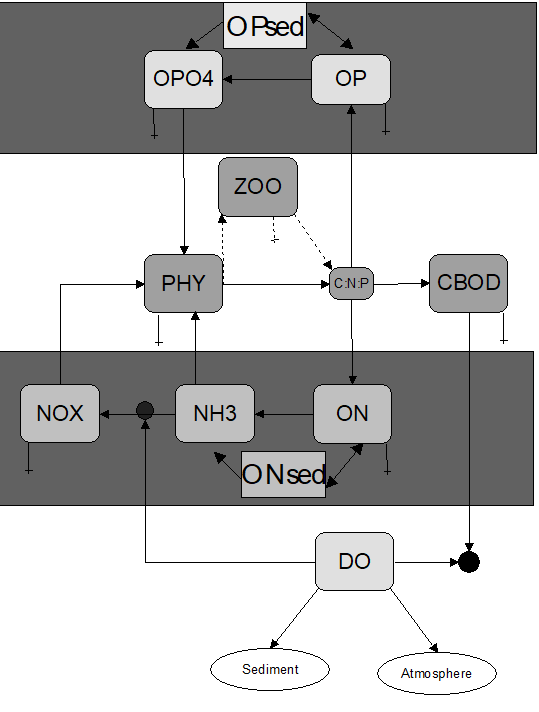
\includegraphics[scale=1]{eutro.png}
\caption{The overall structure of the EUTRO module with state variables (grey boxes), fluxes of matter (arrows). Black circles represent oxygen consumption in nitrification and in the degradation of organic matter. }
\label{eutro_scheme}
\end{figure}

The model implementation allows to vary the represented complexity, by switching the state variables on and off.
Phytoplankton (Table 1) is driven by the anabolic and the catabolic terms, plus a grazing term related to zooplankton concentration (Reaction 10, 11 and 14, \Ttwoa). The anabolic term is related to light intensity, temperature and concentration of nutrients in water, while the catabolic term depends on temperature (\Ttwoa) .
Phytoplankton growth is described by combining a maximum growth rate under optimal conditions, and a number of dimensionless factors, each ranging from 0 to 1, related to specific environmental factors (nutrient, light availability), reducing the phytoplanktonic growth when environmental conditions are suboptimal. Inorganic phosphorous and nitrogen availability on phytoplankton growth/nutrients uptake is simulated by means of Michealis-Menten-Monod kinetics (Table 2). Phytoplankton uptake nitrogen both in the forms of ammonia and nitrate, but ammonia is assimilated preferentially, as indicated in the ammonia preference relation (Reaction. 35, \Ttwoa). Temperature influence on phytoplankton growth is expressed using an exponential relation (Reaction 10, \Ttwoa), light limitation can be chosen between two alternative options (Di Toro and Smith subroutines, Reaction 41, \Ttwoa). 
Nitrogen and phosphorous are then returned to the organic compartment (ON, OP) via phytoplankton and zooplankton respiration and death. After mineralization, the organic form is again converted in the dissolved inorganic form available for phytoplankton growth. 
The DO mass balance is influenced by the reareation rate, due to the exchange with the atmosphere, and photosynthesis (sources of DO) and by respiration and mineralization of particulated and dissolved organic matter (sinks of DO). Other terms included in the DO mass balance are the ones referring to redox reactions such as nitrification and denitrification. The reaeration rate is computed taking into account the wind and current speeds, depth and temperature.
The dynamic of a generic pool of herbivorous zooplankton is simulated with the variable ZOO. Zooplankton grazing has been described by means of a type II functional relationship.
Grazed phytoplankton is assimilated according to the efficiency coefficient EFF. The not assimilated fraction is transferred to the organic matter compartments. Finally, zooplankton mortality is described by a first order kinetics. 


%------------------------------------------------------------------------
%
%    Copyright (C) 1985-2020  Georg Umgiesser
%
%    This file is part of SHYFEM.
%
%    SHYFEM is free software: you can redistribute it and/or modify
%    it under the terms of the GNU General Public License as published by
%    the Free Software Foundation, either version 3 of the License, or
%    (at your option) any later version.
%
%    SHYFEM is distributed in the hope that it will be useful,
%    but WITHOUT ANY WARRANTY; without even the implied warranty of
%    MERCHANTABILITY or FITNESS FOR A PARTICULAR PURPOSE. See the
%    GNU General Public License for more details.
%
%    You should have received a copy of the GNU General Public License
%    along with SHYFEM. Please see the file COPYING in the main directory.
%    If not, see <http://www.gnu.org/licenses/>.
%
%    Contributions to this file can be found below in the revision log.
%
%------------------------------------------------------------------------

%\documentclass{report}
%\usepackage{a4}
%\usepackage{shortvrb}
%\begin{document}



\newcommand{\Otwo}{O${}_{2}$}
\newcommand{\Degree}{${}^{o}$}
\newcommand{\power}[1]{${}^{#1}$}

\newcommand{\opn}{ {} }


\newcommand{\VSPGB}{\vspace{0.2cm}}
\newcommand{\HSP}{\hspace*{1.5cm}}
\newcommand{\HHSP}{\hspace*{0.5cm}}
\newcommand{\GBox}[2]{\parbox{#1 cm}{\VSPGB#2\VSPGB}}
\newcommand{\GDBox}[1]{\GBox{5}{#1}}
\newcommand{\GEBox}[1]{\GBox{7}{#1}}
\newcommand{\GFBox}[1]{\GBox{7}{#1}}



\begin{table}\centering
\begin{tabular}{lll}
\hline


& & \\
$\frac{\partial S}{\partial t} =Q(S)$
& &
General Reactor Equation
\\
& & \\

$Q(PHY) = GPP - DPP - GRZ$
& 1 & 
Phytoplankton PHY [mg C/L]
\\

$Q(ZOO) = GZ - DZ$
& 2 &
Zooplankton ZOO [mg C/L]
\\

$Q(NH3) = N_{alg1} + ON1 - N_{alg2} - N1$
& 3 &
Ammonia NH3 [mg N/L]
\\

$Q(NOX) = N1 - NO_{alg} - NIT1$
& 4 &
Nitrate NOX [mg N/L]
\\

$Q(ON) = ON_{alg} - ON1$
& 5 &
Organic Nitrogen ON [mg N/L]
\\

$Q(OPO4) = OP_{alg1} + OP1 - OP_{alg2}$ 
& 6 &
\GBox{5}{
Inorganic Phosphorous OPO4 \\
\HHSP [mg P/L]
}
\\

$Q(OP) = OP_{alg3} - OP1$
& 7 &
Organic Phosphorous OP [mg P/L]
\\

$Q(CBOD) = C1 - OX - NIT2$
& 8 &
\GBox{5}{
Carbonaceous Biological Oxygen \\
\HHSP Demand CBOD [mg \Otwo/L]
}
\\

\GBox{6}{
$Q(DO) = DO1 + DO2 + DO3 $\\
\HSP $\opn - DO4 - N2 - OX - SOD$
}
& 9 &
Dissolved Oxygen DO [mg \Otwo/L]
\\


\hline
\end{tabular}
\caption{Mass balances}
\label{MassBalance}
\end{table}






\begin{table}\centering
\begin{tabular}{lll}
\hline


$GPP=GP1*PHY $
& 10 &
phytoplankton growth
\\

$DPP=DP1*PHY $
& 11 &
phytoplankton death 
\\

$GRZ=KGRZ*\frac{PHY}{PHY+KPZ}*ZOO$
& 12 &
grazing rate coefficient
\\

$GP1=L_{nut} *L_{light} *K1C*K1T^{(T-T_{0} )} $
& 13 &
\GDBox{
phytoplankton growth rate with nutrient and light limitation
}
\\

$DP1=RES+K1D$ 
& 14 &
\GDBox{
phytoplankton respiration and death rate
}
\\

$GZ=EFF*GRZ$ 
& 15 &
zooplankton growth rate
\\

$DZ=KDZ*ZOO$ 
& 16 &
zooplankton death rate
\\

$Z_{ineff} = (1-EFF)*GRZ $
& 17 &
grazing inefficiency on phytoplankton
\\

$Z_{sink} = Z_{ineff}+DZ $
& 18 &
sink of zooplankton
\\

$N_{alg1}= NC*DPP*(1-FON) $
& 19 &
source of ammonia from algal 
death
\\

$N_{alg2}=PN*NC*GPP $
& 20 &
sink of ammonia for algal growth
\\

$NO_{alg}= (1. - PN)*NC*GPP $
& 21 &
sink of nitrate for algal growth
\\

$ON_{alg}= NC*(DPP*FON+Z_{sink}) $
& 22 &
\GDBox{
source of organic nitrogen from phytoplankton and zooplankton death
}
\\

\GBox{5}{
$N1=KC_{nit} *KT_{nit}^{(T-T_{0})} *NH3$
\HSP $\opn *\frac{DO}{K_{nit}+DO}$
}
& 23 &
nitrification
\\

\GBox{5}{
$NIT1=KC_{denit} KT_{denit}^{(T-T_{0})}$
\HSP $\opn *NOX*\frac{K_{denit}}{K_{denit}+DO}$
}
& 24 &
denitrification
\\

$ON1=KNC_{\min } *KNT_{\min }^{(T-T_{0})} *ON$
& 25 &
mineralization of ON
\\

$OP1=KPC_{\min } *KPT_{\min } ^{(T-T_{0})} *OP$
& 26 &
mineralization of OP
\\

$OP_{alg1}=PC*DPP*(1. - FOP) $
& 27 &
\GDBox{
source of inorganic phosphorous from algal death
}
\\

$OP_{alg2}=PC*GPP $
& 28 &
\GDBox{
sink of inorganic phosphorous for algal growth
}
\\

$OP_{alg3}=PC*(DPP*FOP+Z_{sink}) $
& 29 &
\GDBox{
source of organic phosphorous from phytoplankton and zooplankton death
}
\\

\GBox{5}{
$OX=KDC*KDT^{(T-T_{0} )} $
\HSP $\opn *CBOD*\frac{DO}{KBOD+DO} $
}
& 30 &
oxidation of CBOD
\\

\hline
\end{tabular}
\caption{Functional Expression Description}
\label{FuncDesc}
\end{table}

\begin{table}\centering
\begin{tabular}{lll}
\hline

$C1=OC*(K1D*PHY+Z_{sink}) $
& 31 &
\GDBox{
source of CBOD from phytoplankton and zooplankton death
}
\\

$NIT2=\left( \frac{5}{4} *\frac{32}{14} *NIT1\right) $
& 32 &
sink of CBOD due to denitrification
\\

$DO1=KA*(O_{sat} - DO) $
& 33 &
reareation term
\\

$DO2=PN*GP1*PHY*OC $
& 34 &
\GDBox{
dissolved oxygen produced by phytoplankton using NH3
}
\\

\GBox{5}{
$DO3=(1-PN)*GP1*PHY$
\HSP $\opn * 32*\left( \frac{1}{12} +1.5*\frac{NC}{14} \right) $
}
& 35 &
growth of phytoplankton using NOX
\\

$DO4 = OC*RES*PHY$ 
& 36 &
respiration term
\\

$N2=\left( \frac{64}{14} *N1\right) $
& 37 &
oxygen consumption due to nitrification
\\

\GBox{6}{
$PN=\frac{NH3*NOX}{(KN+NH3)*(KN+NOX)}$ 
\HSP $\opn +\frac{NH3*KN}{(NH3+NOX)*(KN+NOX)} $
}
& 38 &
ammonia preference
\\

$RES=K1RC*K1RT^{(T-T_{0})} $
& 39 &
algal respiration
\\

$SOD=\frac{SOD1}{H} *SODT^{(T-T_{0})} $
& 40 &
sediment oxygen demand
\\

$L_{nut}= min(X1,X2) \, , \,  mult(X1,X2) $
& 41 &
\GDBox{
minimum or multiplicative nutrient limitation for phytoplankton growth
}
\\

$X1=\frac{NH3+NOX}{KN+NH3+NOX} $
& 42 &
\GDBox{
nitrogen limitation for phytoplankton growth
}
\\

$X2=\frac{OPO4}{\frac{KP}{FOPO4} +OPO4} $
& 43 &
\GDBox{
phosphorous limitation for phytoplankton growth
}
\\

$L_{light} =\frac{I_{0} }{I_{s} } *e^{-(KE*H)} *e^{(1-\frac{I_{0} }{I_{s}
} *e^{(-KE*H)} )} $
& 44 &
\GDBox{
light limitation for phytoplankton growth
}
\\

$KA=F(Wind,Vel,T,T_{air},H) $
& 45 &
re-areation coefficient 
\\


\hline
\end{tabular}
\addtocounter{table}{-1}
\caption{(continued) Functional Expression Description}
\label{FuncDesc1}
\end{table}













\begin{table}\centering
\begin{tabular}{ll}
\hline


$K1D=0.12$ day\power{-1}  
&
phytoplankton death rate constant
\\

$KGRZ=1.2$ day\power{-1}  
&
grazing rate constant
\\

$KPZ=0.5$ mg C/L 
&
\GFBox{
half saturation constant for phytoplankton in grazing
}
\\

$KDZ=0.168$ day\power{-1} 
&
zooplankton death rate
\\

$K1C=2.88$ day\power{-1} 
&
phytoplankton growth rate constant
\\

$K1T=1.068$ 
&
\GFBox{
phytoplankton growth rate temperature constant
}
\\

$KN=0.05$ mg N/L 
&
\GFBox{
nitrogen half saturation constant for phytoplankton growth
}
\\

$KP=0.01$ mg P/L 
&
\GFBox{
phosphorous half saturation constant for phytoplankton growth
}
\\

$KC_{nit}=0.05$ day\power{-1} 
&
nitrification rate constant
\\

$KT_{nit}=1.08$ 
&
nitrification rate temperature constant
\\

$K_{nit}=2.0$ mg \Otwo/L 
&
half saturation constant for nitrification
\\

$KC_{denit}=0.09$ day\power{-1} 
&
denitrification rate constant
\\

$KT_{denit}=1.045$ 
&
denitrification rate temperature constant
\\

$K_{denit}=0.1$ mg \Otwo/L 
&
half saturation constant for denitrification
\\

$KNC_{min}=0.075$ day\power{-1} 
&
mineralization of dissolved ON rate constant
\\

$KNT_{min}=1.08$ 
&
\GFBox{
mineralization of dissolved ON rate temperature constant
}
\\

$KDC=0.18$ day\power{-1}
&
oxidation of CBOD rate constant
\\

$KDT= 1.047$ 
&
oxidation of CBOD rate temperature constant
\\

$NC=0.115$ mg N/mg C 
&
N/C ratio
\\

$PC=0.025$ mg P/mg 
&
C P/C ratio
\\

$OC=32/12$ mg \Otwo/mg C 
&
O/C ratio
\\

$EFF=0.5$ 
&
grazing efficiency
\\

$FON=0.5$ 
&
fraction of ON from algal death
\\

$FOP=0.5$ 
&
fraction of OP from algal death
\\

$FOPO4=0.9$ 
&
fraction of dissolved inorganic phosphorous
\\

$KPC_{min}=0.0004$ day\power{-1}  
&
mineralization of dissolved OP rate constant
\\

$KPT_{min}=1.08$ 
&
\GFBox{
mineralization of dissolved OP rate temperature constant
}
\\

$KBOD=0.5$ mg \Otwo/L
&
CBOD half saturation constant for oxidation
\\

$K1RC=0.096$ day\power{-1}  
&
algal respiration rate constant
\\

$K1RT=1.068$ 
&
algal respiration rate temperature constant
\\

$I_{s}=1200000$ lux/day
&
\GFBox{
optimal value of light intensity for phytoplankton growth
}
\\

$KE=1.0$ m\power{-1}
&
light extinction coefficient
\\

\GBox{5}{
$SOD1=2.0$ mg \Otwo/L \\
\HSP day\power{-1} m 
}
&
sediment oxygen demand rate constant
\\

$SODT=1.08$ 
&
sediment oxygen demand temperature constant
\\

$T_{0}=20$ \Degree C 
&
optimal temperature value
\\


\hline
\end{tabular}
\caption{Parameters}
\label{Paras}
\end{table}





\begin{table}\centering
\begin{tabular}{lll}
\hline


$T$ 
& [\Degree C] &
water temperature
\\

$T_{air}$ 
& [\Degree C] &
air temperature
\\

$O_{sat}$  
& [mg/L] &
DO concentration value at saturation
\\

$I_{0}$ 
& [lux/day] &
incident light intensity at the surface
\\

$H$ 
& [m] &
depth
\\

$Vol$ 
& [m\power{3}] &
volume
\\

$Vel$ 
& [m/sec] &
current speed
\\

$Wind$ 
& [m/sec] &
wind speed
\\


\hline
\end{tabular}
\caption{Variables}
\label{Vars}
\end{table}




%\end{document}



\subsubsection{sediment module}
An additional process that can be switched on and off is the evolution of both nitrogen and phosphorus detritus in sediment. The variables  ONsed and OPsed (not subjected to advection-diffusion processes) are used in this case. These two variables interact with the Nitrogen and Phosphorous cycles through the resuspension and sinking of organic N and P, as described by the equations in Table 1. When the wsedim  subroutine is switched on, OP, ON, NH3 and OPO4 are updated at each time step in agreement with those equations. The resuspension is a linear function of the water velocity calculated by the hydrodynamic model at each box, as written in Tab. \ref{MassBalance}. The amount of the sinking nutrients depends on specific parameters, as given in Tab. \Ttwoa, and on the depth of the underlying column.
This routine can be switched on and off as needed by the user, setting the |bsedim|, parameter true or false in the bio3d routine. 

\subsubsection{Parameters for the str file}
Below the parameters to set in the input file |str|


|Ibio=1|		simulate eutro

To set boundary conditions add a section |$bound| and set:

|bio2dn=| File name that contains boundary conditions for concentration of the water quality state variables. The format is the same as for the file boundn. The unit of the values given in the second and following column (9 data columns for EUTRO) must the ones of the variable.

Initialization of variables are done using external files, otherwise are set by default in the code, with uniform value in the domain.  Spatially variable initial conditions should be provided in section |$name|.
\begin{itemize}
\item Name1.bio: File with concentration values of water quality for the initialization.
\item Name1.salt: Files with salinity concentration values [psu] for the initialization.
\item Name1.temp: File with and Temperature values [deg C] for the initialization.
\end{itemize}

%For further details about EUTRO-WASP integration into SHYFEM see \cite{Umgie2003}.


%\subsubsection{ERSEM-BFM}

%The ecosystem model is built on the base of the Biogeochemical Flux Model (ERSEM-BFM), a biomass-based differential equation model. The model is built with respect to mass conservation following a top-down approach, where the food web consists of functional groups defined as Chemical Functional Families and Living Functional Groups. Each group is expressed in terms of basic elements components, such as C, N, P and SI, or by molecules as Chlorophyll, which constitutes a set of state variables. The model simulates the evolution of up to 44 state variables in the water column describing both the main metabolic processes within each functional groups and the predation processes between functional groups. In particular, carbon assimilation, nutrient uptake, analysis of primary producers, grazing by and of secondary producers, respiration, mortality excretion and exudation of all organisms are modelled.

%Only the pelagic foodweb has been considered which is constituted by primary producers, zooplankton, bacteria, nutrients and dissolved chemical species for oxygen and the carbonate system. Primary producers are divided in four principal groups: one silicate dependent group named diatoms and three silicate independent groups named picophytoplankton, flagellates and dinoflagellates. Bacterioplankton represent free-living, non-colonial bacteria that can switch from aerobic to anaerobic metabolism according to the pelagic oxygen conditions. There are four zooplankton groups in the model corresponding to microzooplankton, heterotrophic nanoflagellates, carnivorous mesozooplancton and omnivorous mesozooplancton. The other explicitly simulated environmental variables are nutrients (nitrite, nitrate, ammonium, orthophosphate and silicate. dissolved bioavailable iron), dissolved oxygen, carbon dioxide, dissolved and particulate (non-living) organic matter.

%More information on the ERSEM-BFM ecological module can be found at https://www.nioz.nl/en/about/cos/ecosystem-modelling/ersem-bfm-model


%%%%%%%%%%%%%%%%%%%%%%%%%%%%%%%%%%%%%%%%%%%%%%%%%%%%%%%%%%%%%%%%%%%%%%%%
%%%%%%%%%%%%%%%%%%%%%%%%%%%%%%%%%%%%%%%%%%%%%%%%%%%%%%%%%%%%%%%%%%%%%%%%
%%%%%%%%%%%%%%%%%%%%%%%%%%%%%%%%%%%%%%%%%%%%%%%%%%%%%%%%%%%%%%%%%%%%%%%%

\appendix
\chapter{Hydrodynamic equations and resolution techniques}

      \section{Equations and Boundary Conditions}
	
%------------------------------------------------------------------------
%
%    Copyright (C) 1985-2020  Georg Umgiesser
%
%    This file is part of SHYFEM.
%
%    SHYFEM is free software: you can redistribute it and/or modify
%    it under the terms of the GNU General Public License as published by
%    the Free Software Foundation, either version 3 of the License, or
%    (at your option) any later version.
%
%    SHYFEM is distributed in the hope that it will be useful,
%    but WITHOUT ANY WARRANTY; without even the implied warranty of
%    MERCHANTABILITY or FITNESS FOR A PARTICULAR PURPOSE. See the
%    GNU General Public License for more details.
%
%    You should have received a copy of the GNU General Public License
%    along with SHYFEM. Please see the file COPYING in the main directory.
%    If not, see <http://www.gnu.org/licenses/>.
%
%    Contributions to this file can be found below in the revision log.
%
%------------------------------------------------------------------------

%%%%%%%%%%%%%%%%%%%%%%%%%%%%%%%%%%%%%%%%%%%%%%%%%%%%%%%%%%
%%%%%%% user commands %%%%%%%%%%%%%%%%%%%%%%%%%%%%%%%%%%%%
%%%%%%%%%%%%%%%%%%%%%%%%%%%%%%%%%%%%%%%%%%%%%%%%%%%%%%%%%%

\newcommand{\paren}[1]	{ \left( #1 \right) }
\newcommand{\mez}{\mbox{$\frac{1}{2}$}}
\newcommand{\dpp}{\mbox{$\partial$}}
\newcommand{\zz}{\zeta}
\newcommand{\un}{\mbox{$U^{n+1}$}}
\newcommand{\uo}{\mbox{$U^{n}$}}
\newcommand{\vn}{\mbox{$V^{n+1}$}}
\newcommand{\vo}{\mbox{$V^{n}$}}
\newcommand{\zn}{\mbox{$\zz^{n+1}$}}
\newcommand{\zo}{\mbox{$\zz^{n}$}}
\newcommand{\up}{\mbox{$U^{\prime}$}}
\newcommand{\vp}{\mbox{$V^{\prime}$}}
\newcommand{\zp}{\mbox{$\zz^{\prime}$}}
\newcommand{\dzxp}{\mez \frac{\dpp (\zn + \zo)}{\dpp x}}
\newcommand{\dzyp}{\mez \frac{\dpp (\zn + \zo)}{\dpp y}}
\newcommand{\dzxn}{\mbox{$\frac{\dpp \zn}{\dpp x}$}}
\newcommand{\dzyn}{\mbox{$\frac{\dpp \zn}{\dpp y}$}}
\newcommand{\dzxo}{\mbox{$\frac{\dpp \zo}{\dpp x}$}}
\newcommand{\dzyo}{\mbox{$\frac{\dpp \zo}{\dpp y}$}}

\newcommand{\tdif}[1] {\frac{\partial #1}{\partial t}}
\newcommand{\xdif}[1] {\frac{\partial #1}{\partial x}}
\newcommand{\ydif}[1] {\frac{\partial #1}{\partial y}}
\newcommand{\zdif}[1] {\frac{\partial #1}{\partial z}}
\newcommand{\xxdif}[1] {\frac{\partial^2 #1}{\partial {x}^2}}
\newcommand{\yydif}[1] {\frac{\partial^2 #1}{\partial {y}^2}}
\newcommand{\dt} {\mbox{$\Delta t$}}
\newcommand{\dthalf} {\mbox{$\frac{\Delta t}{2}$}}
\newcommand{\dtt} {\mbox{$\frac{\Delta t}{2}$}}
\newcommand{\dx} {\mbox{$\Delta x$}}
\newcommand{\dy} {\mbox{$\Delta y$}}

\newcommand{\beq} {\begin{equation}}
\newcommand{\eeq} {\end{equation}}
\newcommand{\beqa} {\begin{eqnarray}}
\newcommand{\eeqa} {\end{eqnarray}}

\newcommand{\olds} {\mbox{$\scriptstyle (0)$}}
\newcommand{\news} {\mbox{$\scriptstyle (1)$}}
\newcommand{\meds} {\mbox{$\scriptscriptstyle (\frac{1}{2})$}}
\newcommand{\half} {\mbox{$\scriptstyle \frac{1}{2}$}}

\newcommand{\nsz} {\normalsize}
\newcommand{\uold} {\mbox{$U^{\olds}$}}
\newcommand{\vold} {\mbox{$V^{\olds}$}}
\newcommand{\unew} {\mbox{$U^{\news}$}}
\newcommand{\vnew} {\mbox{$V^{\news}$}}
\newcommand{\zold} {\zeta^{(0)}}
\newcommand{\znew} {\zeta^{(1)}}
\newcommand{\resr} {{\cal R}}
\newcommand{\drho} {\frac{1}{\rho_{0}}}
\newcommand{\fracs}[2] {\mbox{$\frac{#1}{#2}$}}
%\newcommand{\deltat} {\mbox{$\tilde{\delta}$}}
%\newcommand{\gammat} {\mbox{$\tilde{\gamma}$}}
\newcommand{\ffxx} {\tilde{f_x}}
\newcommand{\ffyy} {\tilde{f_y}}

\newcommand{\uv} {{\bf U}}
\newcommand{\uvold} {{\bf U^{(0)}}}
\newcommand{\uvnew} {{\bf U^{(1)}}}
\newcommand{\af} {\alpha_{f}}
\newcommand{\ac} {\alpha_{c}}
\newcommand{\am} {\alpha_{m}}
\newcommand{\duv} {\Delta {\bf U}}
\newcommand{\dzeta} {\Delta \zeta}
\newcommand{\iv} {{\bf I}}
\newcommand{\ivh} {\hat{\bf I}}
\newcommand{\fv} {{\bf F}}
\newcommand{\uvh} {\hat{\bf U}}


%%%%%%%%%%%%%%%%%%%%%%%%%%%%%%%%%%%%%%%%%%%%%%%%%%%%%%%%%%
%%%%%%% hyphenation %%%%%%%%%%%%%%%%%%%%%%%%%%%%%%%%%%%%%%
%%%%%%%%%%%%%%%%%%%%%%%%%%%%%%%%%%%%%%%%%%%%%%%%%%%%%%%%%%

%DEB
The equations of motion for an incompressible Boussinesq flow comprise the 3D equations of momentum balance.
The equations, integrated over each layer, read:

%\beq \label{ubarocl}
\begin{subequations}
\begin{eqnarray}
\tdif{U_l} +Adv_l^{x} -fV_l =  -gh_l \xdif{\zeta} -\frac{gh_l}{\rho_0}\int_{-H_l}^{\zeta} \rho^{'} dz + \nonumber \\
-\frac{h_l}{\rho_0} \xdif{p_a} +A_H(\xxdif{U_l}+\yydif{U_l}) + \frac{1}{\rho_0}(\tau_x^{top(l)} -\tau_x^{bottom(l)}) \\ \nonumber
~~~~\\  \nonumber \\
\tdif{V_l} +Adv_l^{y} +fU_l = -gh_l \ydif{\zeta} -\frac{gh_l}{\rho_0}\int_{-H_l}^{\zeta} \rho^{'} dz + \nonumber \\
-\frac{h_l}{\rho_0} \ydif{p_a}+A_H(\xxdif{V_l}+\yydif{V_l}) +\frac{1}{\rho_0}(\tau_y^{top(l)} -\tau_y^{bottom(l)}) \\ \nonumber
\end{eqnarray}
\end{subequations}

with l vertical layer, ($U_l$, $V_l$) horizontal velocities are integrated over the layer (transports),

\[
 U_l = \int_{-H_l}^{-H_{l-1}} u_l \: dz \; \hspace{1.cm}
 V_l =  \int_{-H_l}^{-H_{l-1}} v_l \: dz \;
\]

and $p_a$ atmospheric pressure, $g$ gravitational constant, $f$ Coriolis parameter, $\zeta$ sea level, $\rho_0$ the constant water density,
$\rho = \rho_0 + \rho^{'}$, $h_l$ layer thickness, $H_l$ depth of the bottom of layer $l$, and $A_H$ horizontal eddy viscosity. In addition

\beq
Adv_l^{x}= u_{l}\xdif{U_l} +v_{l}\ydif{U_l}+\int_{z_l}^{z_{l-1}} w\zdif{u}dz
\eeq
\beq
Adv_l^{y}= u_{l}\xdif{V_l} +v_{l}\ydif{V_l}+\int_{z_l}^{z_{l-1}} w\zdif{v}dz
\eeq

and the turbulent shear stresses, for each layer are

\beqa
\tau_{x}^{top(l)}= \rho_{0}A_{\nu}\zdif{u_{l-1}},       \tau_{y}^{top(l)}=  \rho_{0}A_{\nu}\zdif{v_{l-1}}\\
\tau_{x}^{bottom(l)}=  \rho_{0}A_{\nu}\zdif{u_{l}},	\tau_{y}^{bottom(l)}=  \rho_{0}A_{\nu}\zdif{v_{l}},
\eeqa

The boundary conditions for stress terms are
\beqa
\tau_{x}^{top(0)}= C_D \rho_a w_x\sqrt{w_x^2+w_y^2},  \tau_{y}^{top(0)}= C_D \rho_a w_y\sqrt{w_x^2+w_y^2} \\
\tau_{x}^{bottom(L)}= C_B \rho_0 (u)_L \sqrt{u_L^2+v_L^2},  \tau_{y}^{bottom(L)}= C_B \rho_0 (v)_L \sqrt{u_L^2+v_L^2},
\eeqa

$C_D$ is the wind drag coefficient, $C_B$ is the bottom friction coefficient, $\rho_a$ is the air density, $(w_x,w_y)$ is the wind
velocity 10 m above the sea surface, and $(u_L, v_L)$ is the bottom velocity.

The continuity equation integrated over a vertical layer l is written as:
\beq
\xdif{U_l}+\ydif{V_l}=w_l-w_{l-1}
\eeq

The integration of the continuity equation vertically over the water column provides an equation for the water level t the free surface
\beq
\tdif{\zeta}+\xdif{\int_{-H}^{\zeta}u dz}+\ydif{\int_{-H}^{\zeta}v dz} = P-E
\eeq

where $E$ is evaporation and $P$ is precipitation.

The scalar transport and diffusion equations, are the following:
\beq
\tdif{h_l C_l}+U_l\xdif{C_l}+V_l\ydif{C_l}+\int_{H_{l}}^{H_{l-1}} w\zdif{C_l}=K_H(\xxdif{h_l C_l}+\yydif{h_l C_l})+\int_{H_{l}}^{H_{l-1}} \zdif{K_{\nu}\zdif{C_l}}+ F_s
\eeq
where $C_l$ is the scalar, either salinity, temperature or concentration. $F_s$ is the source term, representing the salinity source or the heat input, for salinity and temperature equations, respectively.


Water levels are prescribed at the open boundaries. At closed boundaries,
the normal velocity component is set to zero whereas the tangential velocity
is a free parameter. This corresponds to a full slip condition.


%%%%%%%%%%%%%%%%%%%%%%%%%%%%%%%%%%%%%%%%%%%%%%%%%%%%%%%%%%%%%%%%%%%%%%%%%
%%%%%%%%%%%%%%%%%%%%%%%%%%%%%%%%%%%%%%%%%%%%%%%%%%%%%%%%%%%%%%%%%%%%%%%%%
%%%%%%%%%%%%%%%%%%%%%%%%%%%%%%%%%%%%%%%%%%%%%%%%%%%%%%%%%%%%%%%%%%%%%%%%%
%%%%%%%%%%%%%%%%%%%%%%%%%%%%%%%%%%%%%%%%%%%%%%%%%%%%%%%%%%%%%%%%%%%%%%%%%
%%%%%%%%%%%%%%%%%%%%%%%%%%%%%%%%%%%%%%%%%%%%%%%%%%%%%%%%%%%%%%%%%%%%%%%%%







	\section{The Model}
	The model uses the semi-implicit time discretization to accomplish
the time integration. A finite element method has been used for the space discretization
 with staggered finite elements instead of its standard formulation. 
In the following a description of the method is given, applying it, 
for simplicity, to the vertically averaged equations of motion.



%%%%%%%%%%%%%%%%%%%%%%%%%%%%%%%%%%%%%%%%%%%%%%%%%%%%%%%%%%%%%%%%%%%%%%%%%
%%%%%%%%%%%%%%%%%%%%%%%%%%%%%%%%%%%%%%%%%%%%%%%%%%%%%%%%%%%%%%%%%%%%%%%%%
%%%%%%%%%%%%%%%%%%%%%%%%%%%%%%%%%%%%%%%%%%%%%%%%%%%%%%%%%%%%%%%%%%%%%%%%%
%%%%%%%%%%%%%%%%%%%%%%%%%%%%%%%%%%%%%%%%%%%%%%%%%%%%%%%%%%%%%%%%%%%%%%%%%
%%%%%%%%%%%%%%%%%%%%%%%%%%%%%%%%%%%%%%%%%%%%%%%%%%%%%%%%%%%%%%%%%%%%%%%%%



\subsection{Discretization in Time - The Semi-Implicit Method}

Looking for an efficient time integration method,
a semi-implicit scheme has been chosen.
The semi-implicit scheme combines the advantages of
the explicit and the implicit schemes. It is unconditionally stable for any
time step $\dt$ chosen and allows the two momentum equations to be
solved explicitly without solving a linear system. 

The only equation
that has to be solved implicitly is the continuity equation. Compared
to a fully implicit solution of the shallow water equations, the dimensions
of the matrix are reduced to one third. Since the solution of a linear
system is roughly proportional to the cube of the dimension of the system,
the saving in computing time is approximately a factor of 30.

It has to be pointed out that it is important not to be limited with the time
step by the CFL criterion for the speed of the external gravity waves
\[
        \dt < \frac{\dx}{\sqrt{gH}}
\]
where $\dx$ is the minimum distance between the nodes in an element.

With the discretization described below, considering a lagoon with  $\dx \approx$ approximately 500m in almost its whole extension and an average depth equals to 1m, so $\dt$ approximately 200sec. But the limitation of the time step can be seen considering more complicated domain examples. For instance, 
for $\dx = 100$ m and $H = 40$ m
the time step criterion would be $\dt < 5$ sec, a
prohibitive small value.

The vertically averaged momentum equations are discretized as follows
\begin{equation}
\label{zn}
\frac{\zn-\zo}{\dt}
                        + \mez \frac{\dpp (\un + \uo)}{\dpp x}
                        + \mez \frac{\dpp (\vn + \vo)}{\dpp y} = 0
\end{equation}
\begin{equation}
\frac{\un-\uo}{\dt} + gH \dzxp + R \un + X = 0
\end{equation}
\begin{equation}
\frac{\vn-\vo}{\dt} + gH \dzyp + R \vn + Y = 0
\end{equation}

With this time discretization the friction term has been formulated
fully implicitly, $X,Y$ fully explicitly and all the other terms
have been centered in time. The reason for the implicit treatment
of the friction term is to avoid a sign inversion in the term when
the friction parameter gets too high. An example of this behavior is
given in Backhaus \cite{Backhaus83}.

If the two momentum equations are solved for the unknowns $\un$ and $\vn$
we have
\begin{equation}
\label{un}
\un = \frac{1}{1+\dt R} \paren{ \uo - \dt gH \dzxp - \dt X }
\end{equation}
\begin{equation}
\label{vn}
\vn = \frac{1}{1+\dt R} \paren{ \vo - \dt gH \dzyp - \dt Y }
\end{equation}

If $\zn$ were known, the solution for
$\un$ and $\vn$ could directly be given. To find $\zn$ we insert
(\ref{un}) and (\ref{vn}) in (\ref{zn}). After some transformations
(\ref{zn}) reads
\begin{eqnarray} \label{zsys}
        \zn
    & - &
        (\dt/2)^{2} \frac{g}{1+\dt R}         \nonumber
	\paren{ \frac{\dpp}{\dpp x}(H \dzxn) + \frac{\dpp}{\dpp y}(H \dzyn) } \\
    & = &
        \zo + (\dt/2)^{2} \frac{g}{1+\dt R}
	\paren{ \frac{\dpp}{\dpp x}(H \dzxo) + \frac{\dpp}{\dpp y}(H \dzyo) } \\
    & - & (\dt/2) \paren{ \frac{2+\dt R}{1+\dt R} }
        \paren{                               \nonumber
          \frac{\dpp \uo}{\dpp x}
        + \frac{\dpp \vo}{\dpp y}
        } \\
    & + & \frac{\dt^{2}}{2(1+\dt R)}            \nonumber
                \paren{ \frac{\dpp X}{\dpp x} + \frac{\dpp Y}{\dpp y} }
\end{eqnarray}

The terms on the left hand side contain the unknown $\zn$, the right hand
contains only known values of the old time level. If the spatial derivatives
are now expressed by the finite element method, a linear system with the unknown
$\zn$ is obtained and can be solved by standard methods. Once the solution
for $\zn$ is obtained it can be substituted into (\ref{un}) and (\ref{vn})
and these two equations can be solved explicitly. In this way all unknowns
of the new time step have been found.

Note that the variable $H$ also contains the water level through
$H=h+\zz$. In order to avoid the equations to become nonlinear $\zz$
is evaluated at the old time level so $H=h+\zo$ and $H$ is a known quantity.


%%%%%%%%%%%%%%%%%%%%%%%%%%%%%%%%%%%%%%%%%%%%%%%%%%%%%%%%%%%%%%%%%%%%%%%%%
%%%%%%%%%%%%%%%%%%%%%%%%%%%%%%%%%%%%%%%%%%%%%%%%%%%%%%%%%%%%%%%%%%%%%%%%%
%%%%%%%%%%%%%%%%%%%%%%%%%%%%%%%%%%%%%%%%%%%%%%%%%%%%%%%%%%%%%%%%%%%%%%%%%
%%%%%%%%%%%%%%%%%%%%%%%%%%%%%%%%%%%%%%%%%%%%%%%%%%%%%%%%%%%%%%%%%%%%%%%%%
%%%%%%%%%%%%%%%%%%%%%%%%%%%%%%%%%%%%%%%%%%%%%%%%%%%%%%%%%%%%%%%%%%%%%%%%%


\subsection{Discretization in Space - The Finite Element Method}


While the time discretization has been explained above, the discretization
in space has still to be carried out. This is done 
using staggered finite elements. 
With the semi-implicit method described above
it is shown below that using linear triangular elements
for all unknowns 
will not be mass conserving. Furthermore the resulting model
will have propagation properties that introduce high numeric damping
in the solution of the equations.

For these reasons a quite new approach has been adopted here. The water
levels and the velocities (transports) are described by using form
functions of different order, being the standard linear form functions
for the water levels but stepwise constant form functions for the
transports. This will result in a grid that resembles more a staggered
grid in finite difference discretizations.

\subsubsection{Formalism}

Let $u$ be an approximate solution of a linear differential
equation $L$. We expand $u$ with the help of basis functions $\phi_{m}$
as
\begin{equation}
\label{exp}
	u=\phi_{m} u_{m} \mbox{\hspace{1cm}} m=1,K
\end{equation}
where $u_{m}$ is the coefficient of the function $\phi_{m}$ and $K$
is the order of the approximation.
In case of linear finite
elements it will just be the number of nodes of the grid used to
discretize the domain.

To find the values $u_{m}$, we try to minimize the residual
that arises when $u$ is introduced into $L$ multiplying the equation $L$
by some weighting functions $\Psi_{n}$ and
integrating over the whole domain leading to
\begin{equation}
\label{int}
\int_{\Omega} \psi_{n} L(u) \: d\Omega \; = 
\int_{\Omega} \psi_{n} L(\phi_{m} u_{m}) \: d\Omega \;
= u_{m} \int_{\Omega} \psi_{n} L(\phi_{m}) \: d\Omega \;
\end{equation}

If the integral is identified with the elements of a matrix $a_{nm}$
we can write (\ref{int}) also as a linear system
\begin{equation} \label{sys}
	a_{nm}u_{m} = 0 \mbox{\hspace{1cm}} n=1,K \hspace{0.5cm} m=1,K
\end{equation}

Once the basis and weighting functions have been specified the system
may be set up and (\ref{sys}) may be solved for the unknowns $u_{m}$.






\subsubsection{Staggered Finite Elements}

For decades finite elements have been used in fluid mechanics in
a standardized manner.
The form functions $\phi_{m}$ were chosen as continuous piecewise linear
functions allowing a subdivision of the whole area of interest into small
triangular elements specifying the coefficients $u_{m}$ at the vertices
(called nodes)
of the triangles. The functions $\phi_{m}$ are 1 at node
$m$ and 0 at all other nodes and thus different from 0 only in the
triangles containing the node $m$.
An example is given in the upper left part of Fig. \ref{figA}
where the form function for node $i$ is shown. The full circle indicates
the node where the function $\phi_{i}$ take the value
1 and the hollow circles where they are 0.


\begin{figure}
\vspace{5.cm}
\caption{a) form functions in domain \hspace{1.cm} b) domain of
influence of node $i$}
%\end{figure}

\begin{picture}(300,10)

\put(10,30){
\begin{picture}(1,1)
\put(80,90){\line(0,1){30}}
\put(80,90){\line(3,1){30}}
\put(80,90){\line(2,-3){20}}
\put(80,90){\line(-2,-3){20}}
\put(80,90){\line(-3,1){30}}
\put(60,60){\line(1,0){40}}
\put(60,60){\line(1,-2){20}}
\put(60,60){\line(-2,-3){20}}
\put(60,60){\line(-4,1){40}}
\put(60,60){\line(-1,4){10}}
\put(50,100){\line(-1,-1){30}}
\put(50,100){\line(-3,1){30}}
\put(50,100){\line(-1,4){10}}
\put(50,100){\line(3,2){30}}
\put(80,120){\line(-2,1){40}}
\put(80,120){\line(1,3){10}}
\put(80,120){\line(3,-2){30}}
\put(110,100){\line(-2,5){20}}
\put(110,100){\line(1,1){30}}
\put(110,100){\line(1,-1){30}}
\put(110,100){\line(-1,-4){10}}
\put(100,60){\line(4,1){40}}
\put(100,60){\line(3,-4){30}}
\put(100,60){\line(-1,-2){20}}
\put(130,20){\line(1,5){10}}
\put(130,20){\line(-1,0){50}}
\put(140,130){\line(0,-1){60}}
\put(140,130){\line(-5,2){50}}
\put(40,140){\line(5,1){50}}
\put(40,140){\line(-2,-3){20}}
\put(20,110){\line(0,-4){40}}
\put(40,30){\line(-1,2){20}}
\put(40,30){\line(4,-1){40}}
\thicklines
\put(50,120){\line(1,-1){30}}
\put(50,120){\line(1,0){30}}
\put(50,120){\line(-1,2){10}}
\put(50,120){\line(-3,-1){30}}
\put(50,120){\line(-3,-5){30}}
\put(50,120){\line(1,-6){10}}
\put(50,120){\line(0,-1){20}}
\put(100,80){\line(-1,-2){20}}
\put(100,80){\line(3,-4){30}}
\put(100,80){\line(0,-2){20}}
\put(80,40){\line(0,-2){20}}
\put(80,40){\line(1,0){50}}
\put(130,40){\line(0,-2){20}}
\thinlines
\put(100,30){$n$}
\put(45,88){$i$}
\put(5,90){$\phi_{i}$}
\put(100,10){$\psi_{n}$}
%\put(80,90){\circle*{5}}
%\put(60,60){\circle*{5}}
\put(50,100){\circle*{5}}
%\put(80,120){\circle*{5}}
%\put(110,100){\circle*{5}}
%\put(100,60){\circle*{5}}
\put(100,60){\circle*{5}}
\put(80,20){\circle*{5}}
\put(130,20){\circle*{5}}
%\put(50,100){\circle{7}}
\put(80,90){\circle{7}}
\put(80,120){\circle{7}}
\put(60,60){\circle{7}}
\put(20,70){\circle{7}}
\put(20,110){\circle{7}}
\put(40,140){\circle{7}}
\end{picture}}
%\end{center}



%\put(250,30){
\put(200,30){
\begin{picture}(1,1)
\put(80,90){\line(0,1){30}}
\put(80,90){\line(3,1){30}}
\put(80,90){\line(2,-3){20}}
\put(80,90){\line(-2,-3){20}}
\put(80,90){\line(-3,1){30}}
\put(60,60){\line(1,0){40}}
\put(60,60){\line(1,-2){20}}
\put(60,60){\line(-2,-3){20}}
\put(60,60){\line(-4,1){40}}
\put(60,60){\line(-1,4){10}}
\put(50,100){\line(-1,-1){30}}
\put(50,100){\line(-3,1){30}}
\put(50,100){\line(-1,4){10}}
\put(50,100){\line(3,2){30}}
\put(80,120){\line(-2,1){40}}
\put(80,120){\line(1,3){10}}
\put(80,120){\line(3,-2){30}}
\put(110,100){\line(-2,5){20}}
\put(110,100){\line(1,1){30}}
\put(110,100){\line(1,-1){30}}
\put(110,100){\line(-1,-4){10}}
\put(100,60){\line(4,1){40}}
\put(100,60){\line(3,-4){30}}
\put(100,60){\line(-1,-2){20}}
\put(130,20){\line(1,5){10}}
\put(130,20){\line(-1,0){50}}
\put(140,130){\line(0,-1){60}}
\put(140,130){\line(-5,2){50}}
\put(40,140){\line(5,1){50}}
\put(40,140){\line(-2,-3){20}}
\put(20,110){\line(0,-4){40}}
\put(40,30){\line(-1,2){20}}
\put(40,30){\line(4,-1){40}}
\put(85,95){$i$}
\put(53,107){$j$}
\put(80,90){\circle*{5}}
\put(60,60){\circle*{5}}
\put(50,100){\circle*{5}}
\put(80,120){\circle*{5}}
\put(110,100){\circle*{5}}
\put(100,60){\circle*{5}}
\put(50,100){\circle{7}}
\put(80,90){\circle{7}}
\put(80,120){\circle{7}}
\put(60,60){\circle{7}}
\put(20,70){\circle{7}}
\put(20,110){\circle{7}}
\put(40,140){\circle{7}}
\end{picture}}

\end{picture}

\label{figA}
\end{figure}


The contributions $a_{nm}$ to the system matrix
are therefore different from 0 only in
elements containing node $m$ and the evaluation of the matrix elements
can be performed on an element basis where all coefficients and unknowns
are linear functions of $x$ and $y$.

This approach is straightforward but not very satisfying with the
semi-implicit time stepping scheme for reasons explained below.
Therefore,
another way has been followed in the present formulation. The fluid domain
is still divided in triangles and the water levels are still defined
at the nodes of the grid
and represented by piecewise linear interpolating functions
in the internal of each element, i.e.
\[
        \zeta = \zeta_{m} \phi_{m} \hspace{1cm} m=1,K
\]
However, the transports are now
expanded, over each triangle, with piecewise constant
(non continuous) form functions $\psi_{n}$ over the whole domain. We therefore
write
\[
        U = U_{n} \psi_{n} \hspace{1cm} n=1,J
\]
where $n$ is now running over all
triangles and $J$ is the total number of triangles.
An example of $\psi_{n}$ is given in the lower right part of Fig. \ref{figA}.
Note that the form function is constant 1 over the whole element,
but outside the element identically 0. Thus it is discontinuous
at the element borders.

Since we may
identify the center of gravity of the triangle with the point where
the transports $U_{n}$ are defined (contrary to the water levels
$\zeta_{m}$ which are defined on the vertices of the triangles), the
resulting grid may be seen as a staggered grid where the unknowns
are defined on different locations. This kind of grid is usually used
with the finite difference method. With the form functions used here
the grid of the finite element model resembles
very much an Arakawa B-grid that defines the water levels on the center
and the velocities on the four vertices of a square.

Staggered finite elements have been first introduced into
fluid mechanics by Schoenstadt \cite{Schoenstadt80}. 
He showed that the un-staggered
finite element formulation of the shallow water equations has very
poor geostrophic adjustment properties. Williams 
\cite{Williams81a, Williams81b}
proposed a similar algorithm, the one
actually used in this paper, introducing constant form functions for the
velocities. He showed the excellent propagation and geostrophic
adjustment properties of this scheme.


\subsubsection{The Practical Realization}

The integration of the partial differential equation is now performed by
using the subdivision of the domain in elements (triangles). The
water levels $\zeta$ are expanded in piecewise linear functions
$\phi_{m}, \; m=1,K$ and
the transports are expanded in piecewise constant functions
$\psi_{n}, \; n=1,J$ where $K$ and $J$ are the total number of nodes
and elements respectively.

As weighting functions we use $\psi_{n}$ for the momentum equations
and $\phi_{m}$ for the continuity equation. In this way there will
be $K$ equations for the unknowns $\zeta$ (one for each node) and
$J$ equations for the transports (one for each element).

In all cases the consistent mass matrix has been substituted with
the lumped equivalent. This was mainly done
to avoid solving a linear system in the case of the momentum equations.
But it was of use also in the solution of the continuity equation
because the amount of mass relative to 
one node does not depend on the surrounding
nodes. This was important especially for the flood and dry mechanism
in order to conserve mass.


\subsubsection{Finite Element Equations}

If equations (\ref{un},\ref{vn},\ref{zsys}) are multiplied with their
weighting functions and integrated over an element we can write down
the finite element equations. But the solution of the water levels does
actually not use the continuity equation in the form (\ref{zsys}), but
a slightly different formulation. Starting from equation (\ref{zn}),
multiplied by the weighting function $\Phi_{M}$ and integrated over one
element yields


\[
          \int_{\Omega} \Phi_{N} (\zn-\zo) \: d\Omega \;
+ (\dthalf) \int_{\Omega} 
	  \left( 
	   \Phi_{N} \frac{\dpp (\un + \uo)}{\dpp x} 
+          \Phi_{N} \frac{\dpp (\vn + \vo)}{\dpp y} 
          \right)
	  \: d\Omega \;
= 0
\]
If we integrate by parts the last two integrals we obtain
\[
          \int_{\Omega} \Phi_{N} (\zn-\zo) \: d\Omega \;
- (\dthalf) \int_{\Omega} 
	  \left( 
	    \frac{\dpp \Phi_{N}}{\dpp x} (\un+\uo) 
+           \frac{\dpp \Phi_{N}}{\dpp y} (\vn+\vo)
	  \right)
	  \: d\Omega \;
= 0
\]
plus two line integrals, not shown, over the boundary of each element
that specify the normal flux over the three element
sides. In the interior of the domain,
once all contributions of all elements have
been summed, these terms cancel at every node,
leaving only the contribution of the
line integral on the boundary of the domain. There, however, the
boundary condition to impose is exactly no normal flux over
material boundaries. Thus, the contribution of these line integrals
is zero.

If now the expressions for $\un,\vn$ are introduced, we obtain a system
with again only the water levels as unknowns
\beqa
\int_{\Omega} \Phi_{N} \zn \: d\Omega \;
 & + & (\dt/2)^{2} \alpha g 
\int_{\Omega} H ( \xdif{\Phi_{N}} \xdif{\zn}  \nonumber
 + \ydif{\Phi_{N}} \ydif{\zn} ) \: d\Omega \; \\
 & = &
\int_{\Omega} \Phi_{N} \zo \: d\Omega \;	\nonumber
+ (\dt/2)^{2} \alpha g 
\int_{\Omega} H ( \xdif{\Phi_{N}} \xdif{\zo} 
 + \ydif{\Phi_{N}} \ydif{\zo} ) \: d\Omega \;  \\
 & + &
 (\dt/2)(1+\alpha) \int_{\Omega}  
  ( \xdif{\Phi_{N}} \uo + \ydif{\Phi_{N}} \vo ) \: d\Omega \; \\
 & - & (\dt^{2}/2) \alpha \nonumber
\int_{\Omega} ( \xdif{\Phi_{N}} X + \ydif{\Phi_{N}} Y ) \: d\Omega \; 
\eeqa
Here we have introduced the symbol $\alpha$ as a shortcut for
\[
\alpha = \frac{1}{1+\dt R}
\]
The variables and unknowns may now be expanded with their basis
functions and the complete system may be set up.


%%%%%%%%%%%%%%%%%%%%%%%%%%%%%%%%%%%%%%%%%%%%%%%%%%%%%%%%%%%%%%%%%%%%%%%%%
%%%%%%%%%%%%%%%%%%%%%%%%%%%%%%%%%%%%%%%%%%%%%%%%%%%%%%%%%%%%%%%%%%%%%%%%%
%%%%%%%%%%%%%%%%%%%%%%%%%%%%%%%%%%%%%%%%%%%%%%%%%%%%%%%%%%%%%%%%%%%%%%%%%
%%%%%%%%%%%%%%%%%%%%%%%%%%%%%%%%%%%%%%%%%%%%%%%%%%%%%%%%%%%%%%%%%%%%%%%%%
%%%%%%%%%%%%%%%%%%%%%%%%%%%%%%%%%%%%%%%%%%%%%%%%%%%%%%%%%%%%%%%%%%%%%%%%%

\subsection{Mass Conservation}
\label{mass}
It should be pointed out that only through the use of this staggered grid
the semi-implicit time discretization may be implemented in a feasible
manner. If the Galerkin method is applied
 in a naive way to the resulting equation
(\ref{zsys}) (introducing the linear form functions for transports
and water levels and setting up the system matrix),
the model is not mass conserving.
This may be seen in the following way (see Fig. 1b for reference).
In the computation of the water level at
node $i$, only $\zeta$ and transport values
belonging to triangles that contain node $i$ enter the computation
(full circles in Fig. 1b).
But when, in a second step, the barotropic transports
of node $j$ are computed, water levels of nodes that lie further apart
from the original node $i$ are used
(hollow circles in Fig. 1b).
These water levels have not been included in
the computation of $\zeta_i$, the water level at node $i$.
So the computed transports are actually different
from the transports inserted formally in the continuity equation.
The continuity equation is therefore not satisfied.

These contributions of nodes lying further apart could in principle
be accounted for. In this case
not only the triangles
$\Omega_{i}$ around node $i$ but also all the triangles that have
nodes in common with the triangles $\Omega_{i}$ would give
contributions to node $i$, namely all nodes and elements shown
in Fig. 1b.
The result would be
an increase of the bandwidth of the matrix for the $\zeta$ computation
disadvantageous in terms of memory and time requirements.

Using instead the approach of the staggered finite elements, actually
only the water levels of elements around node $i$ are needed for
the computation of the transports in the triangles $\Omega_i$.
In this case the model satisfies the
continuity equation and is perfectly mass conserving.


\subsection{Inter-tidal Flats}

Part of a basin may consist of areas that are
flooded during high tides and emerge as islands at ebb tide. These
inter-tidal flats are quite difficult to handle numerically because
the elements that represent these areas are neither
islands nor water elements. The boundary line defining their
contours is wandering during the evolution
of time and a mathematical model must reproduce this features.

For reasons of computer time savings, a simplified algorithm has been chosen
to represent the inter-tidal flats. When the water level in at least
one of the three nodes of an element falls below a minimum value (5 cm)
the element is considered an island and is taken out of the system.
It will be reintroduced only when in all three
nodes the water level is again higher then the minimum value.
Because in dry nodes no water level is computed anymore, an estimate
of the water level has to be given with some sort of extrapolation mechanism
using the water nodes nearby.

This algorithm has the advantage that it is very easy to
implement and very fast. The dynamical features close to the
inter-tidal flats are of course not well reproduced but the
behavior of the method for the rest of the domain
gave satisfactory results.

In any case, since the method stores the water levels of the
last time step, before the element is switched off, introducing the
element in a later moment with the same water levels conserves the
mass balance. This method showed a much better performance
than the one where the new elements were introduced with the water
levels taken from the extrapolation of the surrounding nodes.

%%%%%%%%%%%%%%%%%%%%%%%%%%%%%%%%%%%%%%%%%%%%%%%%%%%%%%%%%%%%%%%%%%%%%%%%%
%%%%%%%%%%%%%%%%%%%%%%%%%%%%%%%%%%%%%%%%%%%%%%%%%%%%%%%%%%%%%%%%%%%%%%%%%
%%%%%%%%%%%%%%%%%%%%%%%%%%%%%%%%%%%%%%%%%%%%%%%%%%%%%%%%%%%%%%%%%%%%%%%%%
%%%%%%%%%%%%%%%%%%%%%%%%%%%%%%%%%%%%%%%%%%%%%%%%%%%%%%%%%%%%%%%%%%%%%%%%%
%%%%%%%%%%%%%%%%%%%%%%%%%%%%%%%%%%%%%%%%%%%%%%%%%%%%%%%%%%%%%%%%%%%%%%%%%



\chapter{File Formats}
	\section{GRD file}
	
%------------------------------------------------------------------------
%
%    Copyright (C) 1985-2020  Georg Umgiesser
%
%    This file is part of SHYFEM.
%
%    SHYFEM is free software: you can redistribute it and/or modify
%    it under the terms of the GNU General Public License as published by
%    the Free Software Foundation, either version 3 of the License, or
%    (at your option) any later version.
%
%    SHYFEM is distributed in the hope that it will be useful,
%    but WITHOUT ANY WARRANTY; without even the implied warranty of
%    MERCHANTABILITY or FITNESS FOR A PARTICULAR PURPOSE. See the
%    GNU General Public License for more details.
%
%    You should have received a copy of the GNU General Public License
%    along with SHYFEM. Please see the file COPYING in the main directory.
%    If not, see <http://www.gnu.org/licenses/>.
%
%    Contributions to this file can be found below in the revision log.
%
%------------------------------------------------------------------------
\label{grid}
The SHYFEM grid files have a defined format and file extension (.grd). Below the grd file format is expressed. 
The names used are described in the legend:
\begin{code}
n	item number (node, element, line)
t	type
d	depth
x,y	coordinates
ntot	number of following nodes
n1,n2	node numbers
\end{code}

The format of lines in input file is:

\begin{code}
comment:

0 [anything]

node:

1	n	t	x	y	[d]

element:

2	n	t	ntot	n1 n2 n3 ... 	[d]

line:

3	n	t	ntot	n1 n2 ...	[d]


\end{code}
Be careful about the following:
\begin{itemize}
\item Lines may be split at any point, except before optional argument.
\item d must not be on separate line.
\item If line is split, the continuation line(s) must start with a blank.
\item Blank lines can be inserted as needed
\item if d is not specified, -999. will be used (flag)
\item use t=0 if you do not know what to use
\item n must be unique for every item type 
\item item numbers need not be consecutive
\item the sequence of items is not important, 
nodes can be mixed with elements/lines
\item the minimum number of nodes for element items is 3
\item the minimum number of nodes for line items is 2
\item element items should have all nodes unique
\item line items with the same first and last node are considered closed
\end{itemize}

Examples of grd file format is given below.
\begin{code}
example 1 :

0 example of one line

1 11 0 10. 10.
1 12 0 20. 20.

3 7 0 2 11 12

#----------------

example 2 :

0 example of one element with continuation line

1 11 0 10. 10.
1 12 0 20. 20.
1 15 0 10. 20.

2 7 0 3 
   11 12 15

=============================================================

\end{code}



	\section{FEM file}
	The FEM file uses an optimized way of specifying variables that can be used
in SHYFEM for setting boundary and initial conditions. For 3D files, only
variables that are exisiting are stored. This makes a big difference
when using zeta coordinates, because in the coastal zone many deep
layers are not existing.

The FEM file is headerless. What that means is that the whole file
has no specific header, whereas the single records have headers. This
feature makes it easy to combine different fem files together. If there
are two files of the same variable (say temperature) of different years
(|temp2018.fem|, |temp2019.fem|), combining them is as easy as

|cat temp2018.fem temp2019.fem > combined.fem|. 

The only thing that has
to be taken care of is that the time records could not be unique (there
might be two time records with the same time step), but this
can be handled in a second step with the program femelab:

|femelab -checkdt -out combined.fem|

which will write a new file |out.fem| with unique time stamps.

All routines to write FEM files can be found in |fem3d/subfemfile.f|.
In the same file also documentation can be found on the file format.
In the file |femutil/femfiles/profile.f| examples of how to write
FEM files can be found.

Each FEM file consists of time records:

\begin{verbatim}
!       time record 1
!       time record 2
!       time record ...
\end{verbatim}

The format of each time record is as follows:

\begin{verbatim}
!       header record
!       data record for variable 1
!       data record for variable 2
!       data record for variable ...
!       data record for variable nvar
\end{verbatim}

The format of the header is

\begin{verbatim}
!       dtime,nvers,idfem,np,lmax,nvar,ntype
!       date,time                          for ntype == 1
!       (hlv(l),l=1,lmax)                  only if( lmax > 1 )
!       regpar                             for ntype == 10
\end{verbatim}

For the explaination of the meaning of the various parameters please
see the legend below. |nvers| is a version number of the FEM files. Presently,
the version is 3.

The format of the data record depends on |lmax| which is 1 for 2D data
fields and greater than 1 for 3D fields:

\begin{verbatim}
!       if( lmax == 1 )
!               string
!               np,lmax                    only for nvers > 2
!               (data(1,k),k=1,np)
!       if( lmax > 1 )
!               string
!               np,lmax                    only for nvers > 2
!               do k=1,np
!                 lm,hd(k),(data(l,k),l=1,lm)
!               end do
\end{verbatim}

The meaning of the various parameters can be found here in the legend.
All variables and parameters are integer except where otherwise indicated.

\begin{verbatim}
! dtime         time stamp (double precision, seconds)
! nvers         version of file format
! idfem         id to identify fem file (must be 957839)
! np            number of horizontal points given
! lmax          maximum number of layers given (1 for 2D)
! nvar          number of variables in time record
! ntype         type of data, defines extra data to follow
! date          reference date (integer, YYYYMMDD)
! time          reference time (integer, hhmmss)
! hlv           layer depths (the bottom of each layer)
! string        string with description of data (character*80)
! ilhkv(k)      total number of levels of node k (1 for 2D)
! hd(k)         total depth in node k (real, -999 if unknown)
! data(l,k)     data for variable at level l and node k (real)
! lm            total number of vertical data for point k
! k,l           index for horizontal/vertical dimension
! regpar        regular grid info: nx,ny,x0,y0,dx,dy,flag
! nx,ny         size of regular grid
! x0,y0         origin of regular grid (real)
! dx,dy         space increment of regular grid (real)
! flag          flag for invalid data of regular grid (real)
\end{verbatim}

The meaning of |ntype| is given here:

\begin{verbatim}
! 0             no other lines in header
! 1             give date/time of reference on extra line
! 10            regular grid, info on extra line (regpar)
\end{verbatim}

and combinations are possible. So |ntype=11| means date/time line 
and regular grid.

One clarification on the time specification: the variable |dtime| indicates the
seconds relative to the reference date |date,time|.
Therefore, you can either use |dtime| as time
in seconds referred to the reference date specified with |date,time|. Or you
can set |dtime=0| and specify the date and time of the record in the
|date,time| line. It is also possible to mix both approaches. 

If no reference date is specified, |dtime| refers to the reference
date in the simulation. This approach is not recommended.


	\section{SHY file}
	The SHY file stores the output of the SHYFEM model. It uses an optimized
way of storing variables to save space.  For 3D files, only variables
that are exisiting are stored. This makes a big difference when using
zeta coordinates, because in the coastal zone many deep layers are
not existing.

The SHY file consists of a file header and time records of various
variables.
All routines needed to write SHY files can be found in |fem3d/subshy.f|.
In the same file also documentation can be found on the file format.

Each SHY file consists of the following records:

\begin{verbatim}
!       header record
!       time record 1
!       time record 2
!       time record ...
\end{verbatim}

The time record is structured as follows:

\begin{verbatim}
!       data record for variable 1
!       data record for variable 2
!       data record for variable ...
!       data record for variable nvar
\end{verbatim}

The format of the header is:

\begin{verbatim}
!        write(iunit,err=99) idshy,nvers
!        write(iunit,err=99) ftype
!        write(iunit,err=99) nkn,nel,npr,nlv,nvar
!        write(iunit,err=99) date,time
!        write(iunit,err=99) title
!        write(iunit,err=99) femver
!        write(iunit,err=99) 
!
!        write(iunit,err=99) nen3v
!        write(iunit,err=99) ipev
!        write(iunit,err=99) ipv
!        write(iunit,err=99) iarv
!        write(iunit,err=99) iarnv
!        write(iunit,err=99) xgv
!        write(iunit,err=99) ygv
!        write(iunit,err=99) hm3v
!        write(iunit,err=99) hlv
!        write(iunit,err=99) ilhv
!        write(iunit,err=99) ilhkv
!        write(iunit,err=99) 
\end{verbatim}

For the meaning of the various parameters and variables please
see the legend below. |nvers| is a version number of the SHY files. Presently,
the version is 12.

The format of the data record depends is as follows:

\begin{verbatim}
!        write(iunit,iostat=ierr) dtime,ivar,n,m,lmax
!        if( lmax == 1 ) then
!          write(iunit,iostat=ierr) ( c(1,i),i=1,n*m )
!        else if( m == 1 ) then
!          write(iunit,iostat=ierr) (( c(l,i)
!     +                 ,l=1,il(i) )
!     +                 ,i=1,n )
!        else
!          stop 'error stop: impossible combination of m, lmax'
!        end if
\end{verbatim}

The meaning of the various parameters can be found here in the legend.
All variables and parameters are integer except where otherwise indicated.

\begin{verbatim}
! idshy         id to identify shy file (must be 1617)
! nvers         version of file format
! ftype         type of shy file (see below)
! nkn           total number of nodes
! nel           total number of elements
! npr           either 1 or 3, probably not used
! nlv           total nuber of vertical layers
! nvar          total number of variables in file
! date          reference date (integer, YYYYMMDD)
! time          reference time (integer, hhmmss)
! title         title of simulation (character*80)
! femver        version of shyfem (character*80)
!
! nen3v(3,nel)  element index
! ipev(nel)     external element number
! ipv(nkn)      external node number
! iarv(nel)     element type
! iarnv(nkn)    node type
! xgv(nkn)      x-coordinate (real)
! ygv(nkn)      y-coordinate (real)
! hm3v(3,nel)   depth at each vertex of elements (real)
! hlv(nlv)      layer depths (real, the bottom of each layer)
! ilhv(nel)     total number of layers for each element
! ilhkv(nkn)    total number of layers for each node
!
! dtime         time stamp (double precision, seconds)
! ivar          identification number of variable
! n             total number of horizontal values
! m             can be 1 (normal) or 3 for vertex values
! lmax          maximum number of layers given (1 for 2D)
!
! c(l,i)        data values (real)
! i,l           index for horizontal/vertical dimension
! il(i)         total number of layers for horizontal points
\end{verbatim}

Possible values for |ftype| are:

\begin{verbatim}
! 0             no type
! 1             hydro record (water levels, transports)
! 2             scalar values on nodes
! 3             scalar values on elements
\end{verbatim}




	%\section{STR file}
	%\input{B_str}

\chapter{Input parameter list}
      \section{Parameter list for the SHYFEM model}
        \label{param_list}
	The parameter input file has the extension .str and is composed of different sections, below described. For each section the list of setting parameters that can be declared are presented.
\subsection{Section {\tt \$title}}
\label{parameter}

This section must be always the first section in the parameter input file.
It contains only three lines. An example is given in
\Fig\ref{fig:titleexample}.

\begin{figure}[hbtp]
\begin{verbatim}
$title
        free one line description of simulation
        name_of_simulation
        name_of_basin
$end
\end{verbatim}
\caption{Example of section {\tt \$title}}
\label{fig:titleexample}
\end{figure}

The first line of this section is a free one line description of
the simulation that is to be carried out. The next line contains
the name of the simulation.
All created files will use this name in the main part of the file name
with different extensions. Therefore the hydrodynamic output file
(extension |out|) will be named |name_of_simulation.out|.
The last line gives the name of the basin file to be used. This
is the pre-processed file of the basin with extension |bas|.
In our example the basin file |name_of_basin.bas| is used.

The directory where this files are read from or written to depends
on the settings in section {\tt \$name}. Using the default
the program will read from and write to the current directory.

\subsection{Section {\tt \$para}}
\paragraph{Compulsory time parameters}

This parameters are compulsory parameters that define the
period of the simulation. They must be present in all cases.

\descrpitem{|itanf|}
\descrptext{%
Start of simulation. (Default 0)
}
\par
\descrpitem{|itend|}
\descrptext{%
End of simulation.
}
\par
\descrpitem{|idt|}
\descrptext{%
Time step of integration.
}
\par


\paragraph{Output parameters}

The following parameters deal with the output frequency
and start time to write external files. The content of the various
output files should be looked up in the appropriate section.

If no output time step is decleared, the output file will not be written.
The default value of the output time step is 0., so, if not decleared, there will be no output file. If the time step of the
output files is equal to the time step of the simulation then
at every time step the output file is written. The default start time
of the output is |itanf|, the start of the simulation.

\descrpitem{|idtout|\\|itmout|}
\descrptext{%
Time step and start time for writing to file OUT,
the file containing the general hydrodynamic results.
}
\par

\descrpitem{|idtext|\\|itmext|}
\descrptext{%
Time step and start time for writing to file EXT,
the file containing hydrodynamic data of extra points.
The extra points for which the data is written
to this file are given in section |extra| of
the parameter file.
}
\par

\descrpitem{|idtrst|}
\descrptext{%
Time step for writing the restart
file (extension RST). No restart file is written
with |idtrst| equal to 0. A negative value
is also possible for the time step. In this case
the time step used is |-idtrst|, but the file is
overwritten every time. It therefore contains
always only the last written restart record. The
special value of |idtrst = -1| will write only the
last time step of the simulation in the restart file.
This is useful if you want to start another
simulation from the last output. (Default 0)
}
\par
\descrpitem{|itmrst|}
\descrptext{%
Start time for writing the restart file. If
not given it is the beginning of the simulation.
}
\par
\descrpitem{|itrst|}
\descrptext{%
Time to use for the restart. If a restart
is performed, then the file name containing
the restart data has to be specified in |restrt|
and the time record corresponding to |itrst|
is used in this file. A value of -1 is also possible.
In this case the last record in the restart file
is used for the restart and the simulation starts
from this time. Be aware that this option changes
the parameter |itanf| to the time of the last
record found in |restrt|.
}
\par
\descrpitem{|ityrst|}
\descrptext{%
Type of restart. If 0 and the restart file is not
found the program will exit with an error. Otherwise
the program will simply continue with a cold start.
If |ityrst| is 1 and the given time record is not
found in the file it will exit with error. If
it is 2 it will initialize all values from the
first time record after |itrst|. Therefore, the
value of 2 will guarantee that the program will not
abort and continue running, but it might not
be doing what you intended. (Default 0)
}
\par
\descrpitem{|flgrst|}
\descrptext{%
This variable indicates which variables are read
from the restart file. By default all available
variables are read and used. If some variables
are not wanted (because, e.g., you want to restart
from a different T/S field), this fact can be indicated
in |flgrst|. 1 indicates restart of hydro values,
10 the depth values, 100 T/S values, 1000 the tracer
concentration, 10000 vertical velocities and
100000 the ecological variables. Therefore, a value
of 10111 indicates a restart of everything except
the tracer and the ecological values. The default
value for |flgrst| is -1, which means 111111.
}
\par

\descrpitem{|idtres|\\|itmres|}
\descrptext{%
Time step and start time for writing to file RES,
the file containing residual hydrodynamic data.
}
\par

\descrpitem{|idtrms|\\|itmrms|}
\descrptext{%
Time step and start time for writing to file RMS,
the file containing hydrodynamic data of root mean
square velocities.
}
\par

\descrpitem{|idtflx|\\|itmflx|}
\descrptext{%
Time step and start time for writing to file FLX,
the file containing discharge data through defined
sections.
The transects for which the discharges are computed
are given in section |flux| of
the parameter file.
}
\par

\descrpitem{|idtvol|\\|itmvol|}
\descrptext{%
Time step and start time for writing to file VOL,
the file containing volume information of areas
defined by transects.
The transects that are used to compute the volumes
are given in section |volume| of
the parameter file.
}
\par

\descrpitem{|netcdf|}
\descrptext{%
This parameter chooses output in NetCDF format
if |netcdf| is 1, else the format is unformatted
fortran files. (Default 0)
}
\par

\descrpitem{|idtoff|}
\descrptext{%
handles offline mode (default 0):
\begin{description}
\item[0] do nothing (no offline routines called)
\item[$>$0] write offline data file (.off) with time step |idtoff|.
\item[$<$0] reads offline data from file |offlin|
defined in section |name|. Usage:
\begin{description}
\item[-1] uses offline hydro results
\item[-2] uses offline T/S results
\item[-4] uses offline turbulence results
\end{description}
\end{description}
}
\par

\descrpitem{|itmoff|}
\descrptext{%
Start time for writing to file OFF,
the file containing data for offline runs.
}
\par


\paragraph{General time and date parameters}

A time and date can be assigned to the simulation. These values
refer to the time 0 of the FEM model. The format for the date is
YYYYMMDD and for the time HHMMSS.
You can also give a time zone if your time is not referring to
GMT but to another time zone such as MET.

|date|                The real date corresponding to time 0. (Default 0)
|time|                The real time corresponding to time 0. (Default 0)
|tz|                  The time zone you are in. This is 0 for GMT, 1 for MET
and 2 for MEST (MET summer time). (Default 0)


\paragraph{Model parameters}

The next parameters define the inclusion or exclusion of
certain terms of the primitive equations.

\descrpitem{|ilin|}
\descrptext{%
Linearization of the momentum equations. If |ilin|
is different from 0 the advective terms are not
included in the computation. (Default 1)
}
\par
\descrpitem{|itlin|}
\descrptext{%
This parameter decides how the advective (non-linear)
terms are computed. The value of 0 (default) uses
the usual finite element discretization over a single
element. The value of 1 chooses a semi-lagrangian
approach that is theoretically stable also for
Courant numbers higher than 1. It is however recommended
that the time step is limited using |itsplt| and
|coumax| described below. (Default 0)
}
\par
\descrpitem{|iclin|}
\descrptext{%
Linearization of the continuity equation. If |iclin|
is different from 0 the depth term in the continuity
equation is taken to be constant. (Default 0)
}
\par

The next parameters allow for a variable time step in the
hydrodynamic computations. This is especially important for the
non-linear model (|ilin=0|) as in this case the criterion
for stability cannot be determined a priori and in any case the
time integration will not be unconditionally stable.

The variable time steps allows for longer basic time steps
(here called macro time steps) which have to be set in |idt|.
It then computes the optimal time step (here micro time step)
in order to not exceed the given Courant number. However,
the value for the macro time step will never be exceeded.

Normally time steps are always given in full seconds. This is still
true when specifying the macro time step |idt|.
In older versions, the computed micro time steps also had to be
 full integers. Starting from version 7.1, fractional time steps
were allowed. This allows time steps smaller than 1s.

\descrpitem{|itsplt|}
\descrptext{%
Type of variable time step computation. If this value
is 0, the time step will be kept constant at its initial
value. A value of 1 divides the initial time step into
(possibly) equal parts, but makes sure that at the end
of the micro time steps one complete macro time
step has been executed. The mode |itsplt| = 2
ignores the macro time step, but always
uses the biggest time step possible. In this case,
it is not assured that after some micro time steps
a macro time step will be recovered. Please note
that the initial macro time step will never be exceeded.
In any case, the time step will always be rounded to the
next lower integer value. This is not the case with
|itsplt| = 3 where the highest possible fractional time step
will be used. (Default 0)
}
\par
\descrpitem{|coumax|}
\descrptext{%
Normally the time step is computed in order to not
exceed the Courant number of 1. However, in some cases
the non-linear terms are stable even for a value higher
than 1 or there is a need to achieve a lower Courant number.
Setting |coumax| to the desired Courant number
achieves exactly this effect. (Default 1)
}
\par
\descrpitem{|idtsyn|}
\descrptext{%
In case of |itsplt| = 2 this parameter makes sure that
after a time of |idtsyn| the time step will be syncronized
to this time. Therefore, setting |idtsyn| = 3600 means
that there will be a time stamp every hour, even if the model
has to take one very small time step in order to reach that
time. This parameter is useful
only for |itsplt| = 2 and its default value of
0 does not make any syncronization.
}
\par
\descrpitem{|idtmin|}
\descrptext{%
This variable defines the smallest time step possible
when time step splitting is enabled. Normally the smallest
time step is 1 second. Please set |idtmin| to values
smaller than 1 in order to allow for fractional time steps.
A value of 0.001 allows for timesteps of down to
1 millisecond. (Deault 1)
}
\par

These parameters define the weighting of time level in the
semi-implicit algorithm. With these parameters the damping
of gravity or Rossby waves can be controlled. Only modify them if
you know what you are doing.

\descrpitem{|azpar|}
\descrptext{%
Weighting of the new time level of the transport
terms in the continuity equation. (Default 0.5)
}
\par
\descrpitem{|ampar|}
\descrptext{%
Weighting of the new time level of the pressure
term in the momentum equations. (Default 0.5)
}
\par
\descrpitem{|afpar|}
\descrptext{%
Weighting of the new time level of the Coriolis
term in the momentum equations. (Default 0.5)
}
\par
\descrpitem{|avpar|}
\descrptext{%
Weighting of the new time level of the non-linear
advective terms in the momentum equations. (Default 0.0)
}
\par

The next parameters define the weighting of time level for the
vertical stress and advection terms. They guarantee the stability
of the vertical system. For this reason they are normally set to
1 which corresponds to a fully implicit discretization. Only
modify them if you know what you are doing.

\descrpitem{|atpar|}
\descrptext{%
Weighting of the new time level of the vertical
viscosity in the momentum equation. (Default 1.0)
}
\par
\descrpitem{|adpar|}
\descrptext{%
Weighting of the new time level of the vertical
diffusion in the scalar equations. (Default 1.0)
}
\par
\descrpitem{|aapar|}
\descrptext{%
Weighting of the new time level of the vertical
advection in the scalar equations. (Default 1.0)
}
\par


\paragraph{Coriolis parameters}

The next parameters define the parameters to be used
with the Coriolis terms.

\descrpitem{|icor|}
\descrptext{%
If this parameter is 0, the Coriolis terms are
not included in the computation. A value of 1
uses a beta-plane approximation with a variable
Coriolis parameter $f$, whereas a value of
2 uses an f-plane approximation where the
Coriolis parameter $f$ is kept constant over the
whole domain. (Default 0)
}
\par
\descrpitem{|dlat|}
\descrptext{%
Average latitude of the basin. This is used to
compute the Coriolis parameter $f$. This parameter
is not used if spherical coordinates are used
(|isphe|=1) or if a coordinate 	projection is set
(|iproj| $>$0). (Default 0)
}
\par
\descrpitem{|isphe|}
\descrptext{%
If 0 a cartesian coordinate system is used,
if 1 the coordinates are in the spherical system (lat/lon).
Please note that in case of spherical coordinates the
Coriolis term is always included in the computation, even
with |icor| = 0. If you really do not want to use the
Coriolis term, then please set |icor| = -1. The default is
-1, which means that the type of coordinate system will
be determined automatically.
}
\par


\paragraph{Depth parameters}

The next parameters deal with handling depth values of the basin.

\descrpitem{|href|}
\descrptext{%
Reference depth. If the depth values of the basin and
the water levels are referred to mean sea level, |href|
should be 0 (default value). Else this value is
subtracted from the given depth values. For example,
if |href = 0.20| then a depth value in the basin
of 1 meter will be reduced to 80 centimeters.
}
\par

\descrpitem{|hzmin|}
\descrptext{%
Minimum total water depth that will remain in a
node if the element becomes dry. (Default 0.01 m)
}
\par
\descrpitem{|hzoff|}
\descrptext{%
Total water depth at which an element will be
taken out of the computation because it becomes dry.
(Default 0.05 m)
}
\par
\descrpitem{|hzon|}
\descrptext{%
Total water depth at which a dry element will be
re-inserted into the computation.
(Default 0.10 m)
}
\par

\descrpitem{|hmin|}
\descrptext{%
Minimum water depth (most shallow) for the whole
basin. All depth values of the basin will be adjusted
so that no water depth is shallower than |hmin|.
(Default is no adjustment)
}
\par
\descrpitem{|hmax|}
\descrptext{%
Maximum water depth (deepest) for the whole
basin. All depth values of the basin will be adjusted
so that no water depth is deeper than |hmax|.
(Default is no adjustment)
}
\par

\paragraph{Bottom friction}

The friction term in the momentum equations can be written as
$Ru$ and $Rv$ where $R$ is the variable friction coefficient and
$u,v$ are the velocities in $x,y$ direction respectively.
The form of $R$ can be specified in various ways. The value of
|ireib| is chosen between the formulations. In the parameter
input file a value $\lambda$ is specified that is used in
the formulas below. In a 2D simulation the Strickler (2) or the Chezy (3)
formulation is the preferred option, while for a 3D simulation is
recommended to use the drag coefficient (5) or the roughness length
formulation (6).

\descrpitem{|ireib|}
\descrptext{%
Type of friction used (default 0):
\begin{description}
\item[0] No friction used
\item[1] $R=\lambda$ is constant
\item[2] $\lambda$ is the Strickler coefficient.
In this formulation $R$ is written as
$R = \frac{g}{C^2} \frac{\vert u \vert}{H}$
with $C=k_s H^{1/6}$ and $\lambda=k_s$ is
the Strickler coefficient. In the above
formula $g$ is the gravitational acceleration,
$\vert u \vert$ the modulus of the current velocity
and $H$ the total water depth.
\item[3] $\lambda$ is the Chezy coefficient.
In this formulation $R$ is written as
$R = \frac{g}{C^2} \frac{\vert u \vert}{H}$
and $\lambda=C$ is the Chezy coefficient.
\item[4] $R=\lambda/H$ with $H$ the total water depth
\item[5] $\lambda$ is a constant drag coefficient and $R$ is
computed as $R=\lambda\frac{\vert u \vert}{H}$
\item[6] $\lambda$ is the bottom roughness length and $R$ is
computed through the formula
$R=C\frac{\vert u \vert}{H}$ with
$C=\big(\frac{0.4}{log(\frac{\lambda+0.5H}
{\lambda})}\big)^2$
\item[7] If $\lambda \geq 1$ it specifies the Strickler
coefficient (|ireib=2|), otherwise it specifies a
constant drag coefficient (|ireib=5|).
\end{description}
}
\par
\descrpitem{|czdef|}
\descrptext{%
The default value for the friction parameter $\lambda$.
Depending on the value of |ireib| the coefficient $\lambda$
is representing linear friction, a constant drag coefficient,
the Chezy or Strickler parameter, or the roughness length
(default 0).
}
\par
\descrpitem{|iczv|}
\descrptext{%
Normally the bottom friction coefficient
(such as Strickler, Chezy, etc.)
is evaluated at every time step (|iczv| = 1).
If for some reason this behavior is not desirable,
|iczv| = 0 evaluates this value only before the
first time step, keeping it constant for the
rest of the simulation. Please note that this is
only relevant if you have given more than one bottom
friction value (inflow/outflow) for an area. The
final value of $R$ is computed at every time step
anyway. (default 1)
}
\par

The value of $\lambda$ may be specified for the whole basin through
the value of |czdef|. For more control over the friction parameter
it can be also specified in section |area| where the friction
parameter depending on the type of the element may be varied. Please
see the paragraph on section |area| for more information.

\paragraph{Physical parameters}

The next parameters describe physical values that can be adjusted
if needed.

\descrpitem{|rowass|}
\descrptext{%
Average density of sea water. (Default 1025 \densityunit)
}
\par
\descrpitem{|roluft|}
\descrptext{%
Average density of air. (Default 1.225 \densityunit)
}
\par
\descrpitem{|grav|}
\descrptext{%
Gravitational acceleration. (Default 9.81 \accelunit)
}
\par

\paragraph{Wind parameters}

The next two parameters deal with the wind stress to be
prescribed at the surface of the basin.

The wind data can either be specified in an external file (ASCII
or binary) or directly in the parameter file in section |wind|.
The ASCII file or the wind section contain three columns, the first
giving the time in seconds, and the others the components of
the wind speed. Please see below how the last two columns are
interpreted depending on the value of |iwtype|. For the format
of the binary file please see the relative section.
If both a wind file and section |wind| are given, data from the
file is used.

The wind stress is normally computed with the following formula
\beq
\tau^x = \rho_a c_D \vert u \vert u^x \quad
\tau^y = \rho_a c_D \vert u \vert u^y
\eeq
where $\rho_a,\rho_0$ is the density of air and water respectively,
$u$ the modulus of wind speed and $u^x,u^y$ the components of
wind speed in $x,y$ direction. In this formulation $c_D$ is a
dimensionless drag coefficient that varies between 1.5 \ten{-3} and
3.2 \ten{-3}. The wind speed is normally the wind speed measured
at a height of 10 m.

|iwtype|      The type of wind data given (default 1):
\begin{description}
\item[0] No wind data is processed
\item[1] The components of the wind is given in [m/s]
\item[2] The stress ($\tau^x,\tau^y$) is directly specified
\item[3] The wind is given in speed [m/s] and direction
[degrees]. A direction of 0\degrees{} specifies
a wind from the north, 90\degrees{} a wind
from the east etc.
\item[4] As in 3 but the speed is given in knots
\end{description}
\descrpitem{|itdrag|}
\descrptext{%
Formula to compute the drag coefficient.
\begin{description}
\item[0] constant value given in |dragco|.
\item[1] Smith and Banke (1975) formula
\item[2] Large and Pond (1981) formula
\item[3] Spatio/temporally varing in function of wave. Need
the coupling with WWMIII.
\item[4] Spatial/temporal varying in function of heat flux. Only for iheat = 6 and iheat = 8.
\end{description}
(Default 0)
}
\par
|dragco|      Drag coefficient used in the above formula.
Please note that in case
of |iwtype| = 2 this value is of no interest, since the
stress is specified directly. (Default 2.5E-3)
|wsmax|       Maximum wind speed allowed in [m/s]. This is in order to avoid
errors if the wind data is given in a different format
from the one specified by |iwtype|. (Default 50)

\descrpitem{|wslim|}
\descrptext{%
Limit maximum wind speed to this value [m/s]. This provides
an easy way to exclude strong wind gusts that might
blow up the simulation. Use with caution.
(Default -1, no limitation)
}
\par

\paragraph{Meteo and heat flux parameters}
The next parameters deal with the heat and meteo forcing.

\descrpitem{|iheat|}
\descrptext{%
The type of heat flux algorithm (Default 1):
\begin{description}
\item[1] As in the AREG model
\item[2] As in the POM model
\item[3] Following A. Gill
\item[4] Following Dejak
\item[5] As in the GOTM model
\item[6] Using the COARE3.0 module
\item[7] Read  sensible, latent and longwave fluxes from file
\item[8] Heat flux with bulk-formulae by \cite{Pettenuzzo2010}, computing Net Long wave radiation \cite{Bignami1995}, Sensible heat \cite{Kondo1975}, Latent heat \cite{Kondo1975}, Evaporation \cite{Kondo1975}, Short Wave Solar Radiation \cite{Reed1977}. Selecting iheat = 8 you need to activate also itdrag=4 since the spatial/temporal-varying wind drag coefficient is computed with \cite{Hellermann1983} parametrization, as function of heat flux.
\end{description}
}
\par
\descrpitem{isolp}
\descrptext{%
The type of solar penetration parameterization by one or more exponential decay curves. isolp = 0 sets an e- folding decay of radiation (one exponential decay curve) as function of depth hdecay. isolp = 1 sets a profile of solar radiation with two length scale of penetration. Following the \cite{Jerlov1968} classification the type of water is clear water (type I). (Default 0)
}
\par

\descrpitem{iwtyp}
\descrptext{%
The water types from clear water (type I) to the most turbid water (coastal water 9) following the classification of Jerlov (1968). From clear water type I to type III data are taken from \cite{Paulson1977}. Water type from 1 (option n. 5) to type 9 (option n. 9) were retrieved interpolating Jerlov data so they are still experimental. The possible values for iwtyp are:
\begin{description}
\item[0] clear water type I
\item[1] type IA
\item[2] type IB
\item[3] type II
\item[4] type III
\item[5] type 1
\item[6] type 3
\item[7] type 5
\item[8] type 7
\item[9] type 9
\end{description}
}
\par

\descrpitem{|hdecay|}
\descrptext{%
Depth of e-folding decay of radiation [m]. If |hdecay| = 0
everything is absorbed in first layer (Default 0).
}
\par

\descrpitem{|botabs|}
\descrptext{%
Heat absorption at bottom [fraction] (Default 0).
\begin{description}
\item[=0] everything is absorbed in last layer
\item[=1] bottom absorbs remaining radiation
\end{description}
}
\par

\descrpitem{|albedo|}
\descrptext{%
General albedo (Default 0.06).
}
\par

\descrpitem{|albed4|}
\descrptext{%
Albedo for temp below 4 degrees (Default 0.06).
}
\par

\descrpitem{|imreg|}
\descrptext{%
Regular meteo data (Default 0).
}
\par

\descrpitem{|ievap|}
\descrptext{%
Compute evaporation mass flux (Default 0).
}
\par


\paragraph{Parameters for 3d}
The next parameters deal with the layer structure in 3D.

\descrpitem{|dzreg|}
\descrptext{%
Normally the bottom of the various layers are given in
section |\$levels|. If only a regular vertical grid is desired
then the parameter |dzreg| can be used. It specifies the spacing
of the vertical layers in meters. (Default is 0, which means
that the layers are specified explicitly in |\$levels|.
}
\par

The last layer (bottom layer) is treated in a special way. Depending on
the parameter |ilytyp| there are various cases to be considered. A value
of 0 leaves the last layer as it is, even if the thickness is very small.
A value of 1 will always eliminate the last layer, if it has not full
layer thickness. A value of 2 will do the same, but only if the last layer
is smaller than |hlvmin| (in units of fraction). Finally, a value of
3 will add the last layer to the layer above, if its layer thickness
is smaller than |hlvmin|.

\descrpitem{|ilytyp|}
\descrptext{%
Treatment of last (bottom) layer. 0 means no adjustment,
1 deletes the last layer, if it is not a full layer,
2 only deletes it
if the layer thickness is less than |hlvmin|, and 3
adds the layer thickness to the layer above if it is smaller
than |hlvmin|. Therefore, 1 and 2 might change the
total depth and layer structure, while 3 only might
change the layer structure. The value of 1 will always
give you full layers at the bottom.
}
\par
\descrpitem{|hlvmin|}
\descrptext{%
Minimum layer thickness for last (bottom) layer used when
|ilytyp| is 2 or 3. The unit is fractions of the nominal
layer thickness. Therefore, a value of 0.5 indicates that
the last layer should be at least half of the full
layer.
}
\par

 With $z-$layers the treatment of the free-surface must be addressed.
What happen if the water level falls below the first $z$-level?
A $z-$star type vertical grid deformation can be deployed.
The next parameter specify the number of surface layers that are moving.
\par
\descrpitem{|nzadapt|}
\descrptext{%
Parameter that controls the number of surface $z-$layers that are moving.
The value $|nzadapt|\le 1$ corresponds to standard $z-$layers (Default).
Then, some care is needed to define the first interface sufficiently
deep to avoid the well-known "drying" of the first layer.
The value of $|nzadapt| = N_{tot}$, with $N_{tot}$ the total number
of $z$-layers, is $z-$star (all layers are moving).
Other values of $1<|nzadapt|<N_{tot}$ corresponds to move, at minimum,
the first |nzadapt| surface layers with $z-$star.
These feature is still experimental.
}
\par

The above parameters are dealing with zeta layers, where every layer
has constant thickness, except the surface layer which is varying with
the water level. The next parameters deal with sigma layers where all
layers have varying thickness with the water level.
\par
\descrpitem{|nsigma|}
\descrptext{%
Number of sigma layers for the run. This parameter can
be given in alternative to specifying the sigma layers
in |\$levels|. Only regularly spaced sigma levels
will be created.
}
\par

\par
\descrpitem{|hsigma|}
\descrptext{%
This is still an experimental feature. It allows to use
sigma layers above zeta layers. |hsigma| is the depth where
the transition between these two types of layers
is occurring.
}
\par

The next parameters deal with vertical diffusivity and viscosity.

\descrpitem{|diftur|}
\descrptext{%
Vertical turbulent diffusion parameter for the tracer.
(Default 0)
}
\par
\descrpitem{|difmol|}
\descrptext{%
Vertical molecular diffusion parameter for the tracer.
(Default 1.0e-06)
}
\par
\descrpitem{|vistur|}
\descrptext{%
Vertical turbulent viscosity parameter for the momentum.
(Default 0)
}
\par
\descrpitem{|vismol|}
\descrptext{%
Vertical molecular viscosity parameter for the momentum.
(Default 1.0e-06)
}
\par

\descrpitem{|dhpar|}
\descrptext{%
Horizontal diffusion parameter (general).
(Default 0)
}
\par

The next parameters deal with the control of the scalar transport
and diffusion equation. You have the possibility to prescribe the tvd scheme
desired and to limit the Courant number.

\descrpitem{|itvd|}
\descrptext{%
Type of the horizontal advection scheme used for
the transport and diffusion
equation. Normally an upwind scheme is used (0), but setting
the parameter |itvd| to a value greater than 0
chooses a TVD scheme. A value of 1 will use a TVD scheme
based on the average gradient, and a value of 2 will use
the gradient of the upwind node (recommended).
This feature
is still experimental, so use with care. (Default 0)
}
\par
\descrpitem{|itvdv|}
\descrptext{%
Type of the vertical advection scheme used for
the transport and diffusion
equation. Normally an upwind scheme is used (0), but setting
the parameter |itvd| to 1 chooses a TVD scheme. This feature
is still experimental, so use with care. (Default 0)
}
\par
\descrpitem{|rstol|}
\descrptext{%
Normally the internal time step for scalar advection is
automatically adjusted to produce a Courant number of 1
(marginal stability). You can set |rstol| to a smaller value
if you think there are stability problems. (Default 1)
}
\par


\paragraph{Various parameters}

The next parameters refer to various groups not described previously.

\descrpitem{|tauvel|}
\descrptext{%
If you have velocity observations given in file
|surfvel| then you can specify the relaxation
parameter $\tau$ in the variable |tauvel|. (Default 0,
which means no assimilation of velocities)
}
\par

\descrpitem{|rtide|}
\descrptext{%
If |rtide| = 1 the model calculates equilibrium tidal
potential and load tides and uses these to force the
free surface (Default 0).
}
\par


\paragraph{Temperature and salinity}

The next parameters deal with the transport and diffusion
of temperature and salinity. Please note that in order to compute
T/S, the parameter |ibarcl| must be different from 0. In this case
T/S advection is computed, but may be selectively turned off setting
one of the two parameters |itemp| or |isalt| explicitly to 0.

\descrpitem{|itemp|}
\descrptext{%
Flag if the temperature computation is done.
A value different from 0 computes the temperature transport
and diffusion. (Default 1)
}
\par
\descrpitem{|isalt|}
\descrptext{%
Flag if the salinity computation is done.
A value different from 0 computes the salinity transport
and diffusion. (Default 1)
}
\par

The next parameters set the initial conditions for temperature and salinity.
Both the average value and the stratification can be specified.

\descrpitem{|temref|}
\descrptext{%
Reference (initial) temperature of the water in
centigrade. (Default 0)
}
\par
\descrpitem{|salref|}
\descrptext{%
Reference (initial) salinity of the water in
psu (practical salinity units) or ppt.
(Default 0)
}
\par
\descrpitem{|tstrat|}
\descrptext{%
Initial temperature stratification in units of [C/km].
A positive value indicates a stable stratification.
(Default 0)
}
\par
\descrpitem{|sstrat|}
\descrptext{%
Initial salinity stratification in units of [psu/km].
A positive value indicates a stable stratification.
(Default 0)
}
\par

The next parameters deal with horizontal diffusion of temperature
and salinity. These parameters overwrite the general parameter for
horizontal diffusion |dhpar|.

\descrpitem{|thpar|}
\descrptext{%
Horizontal diffusion parameter for temperature.
(Default 0)
}
\par
\descrpitem{|shpar|}
\descrptext{%
Horizontal diffusion parameter for salinity.
(Default 0)
}
\par


\paragraph{Concentrations}

The next parameters deal with the transport and diffusion
of a conservative substance. The substance is dissolved in
the water and acts like a tracer.

\descrpitem{|iconz|}
\descrptext{%
Flag if the tracer computation is done.
A value different from 0 computes the transport
and diffusion of the substance. If greater than 1
|iconz| concentrations are simulated. (Default 0)
}
\par
\descrpitem{|conref|}
\descrptext{%
Reference (initial) concentration of the tracer in
any unit. (Default 0)
}
\par
\descrpitem{|contau|}
\descrptext{%
If different from 0 simulates decay of concentration. In
this case |contau| is the decay rate (e-folding time) in days.
(Default 0)
}
\par

\descrpitem{|chpar|}
\descrptext{%
Horizontal diffusion parameter for the tracer.
This value overwrites the general parameter for
horizontal diffusion |dhpar|. (Default 0)
}
\par


\paragraph{Output for scalars}

The next parameters define the output frequency of the
computed scalars (temperature, salinity, generic concentration) to file.

\descrpitem{|idtcon|\\|itmcon|}
\descrptext{%
Time step and start time for writing to file
CON (concentration) and NOS (temperature and
salinity).
}
\par

\subsection{Section {\tt \$proj}}
The parameters set in this section handle the projection from cartesian to
geographical coordinate system. If |iproj| $>$0 the projected geographical
coordinates can be used for spatially computing the Coriolis parameter
and tidal potential even if the basin has been set in a cartesian coordinate system
(|isphe| = 0) .

Please find all details here below.

\descrpitem{|iproj|}
\descrptext{%
Switch that indicates the type of projection
(default 0):
\begin{description}
\item[0] do nothing
\item[1] Gauss-Boaga (GB)
\item[2] Universal Transverse Mercator (UTM)
\item[3] Equidistant cylindrical (CPP)
\item[4] UTM non standard
\end{description}
}
\par

\descrpitem{|c\_fuse|}
\descrptext{%
Fuse for GB (1 or 2, default 0)
}
\par

\descrpitem{|c\_zone|}
\descrptext{%
Zone for UTM (1-60, default 0)
}
\par

\descrpitem{|c\_lamb|}
\descrptext{%
Central meridian for non-std UTM (default 0)
}
\par

\descrpitem{|c\_x0|}
\descrptext{%
x0 for GB and UTM (default 0)
}
\par

\descrpitem{|c\_y0|}
\descrptext{%
y0 for GB and UTM (default 0)
}
\par

\descrpitem{|c\_skal|}
\descrptext{%
Scale factor for non-std UTM (default 0.9996)
}
\par

\descrpitem{|c\_phi|}
\descrptext{%
Central parallel for CPP (default 0.9996)
}
\par

\descrpitem{|c\_lon0|}
\descrptext{%
Longitude origin for CPP (default 0)
}
\par

\descrpitem{|c\_lat0|}
\descrptext{%
Latitude origin for CPP (default 0)
}
\par

\subsection{Section {\tt \$waves}}

Parameters in this section activate the wind wave module and define
which kind of wind wave model has to be used. These parameters must
be in section |waves|.

\descrpitem{|iwave|}
\descrptext{%
Type of wind wave model and coupling procedure (default 0):
\begin{description}
    \item[0] No wind wave model called
    \item[1] The parametric wind wave model is called
    (see file subwave.f)
    \item[$>$1] The spectral wind wave model WWMIII is called
    \item[2] ... wind from SHYFEM, radiation stress formulation
    \item[3] ... wind from SHYFEM, vortex force formulation
    \item[4] ... wind from WWMIII, radiation stress formulation
    \item[5] ... wind from WWMIII, vortex force formulation
    \item[11] The spectral wind wave model WaveWatch WW3 is called
\end{description}
}
\par
When the vortex force formulation is chosen the wave-supported
surface stress is subtracted from the wind stress, in order to
avoid double counting of the wind forcing in the flow model.
Moreover, the use of the wave-dependent wind drag coefficient
can be adopted setting |itdrag| = 3.

\descrpitem{|dtwave|}
 \descrptext{%
Time step for coupling with WWMIII. Needed only for
}
\par

 \descrpitem{|iwave|} \descrptext{%
$>$1 (default 0).
}
\par
\descrpitem{|idtwav|} \descrpitem{|itmwav|} \descrptext{%
Time step and start time for writing to file wav,
the files containing output wave variables (significant
wave height, wave period, mean wave direction).
}
\par
\subsection{Section {\tt \$sedtr}}


The following parameters activate the sediment transport module
and define the sediment grain size classes to be simulated.

\descrpitem{|sedtr|}
\descrptext{%
Sediment transport module section name.
}
\par

\descrpitem{|isedi|}
\descrptext{%
Flag if the sediment computation is done:
\begin{description}
\item[0] Do nothing (default)
\item[1] Compute sediment transport
\end{description}
}
\par

\descrpitem{|idtsed|\\|itmsed|}
\descrptext{%
Time step and start time for writing to files sed e sco,
the files containing sediment variables and suspended
sediment concentration.
}
\par

\descrpitem{|sedgrs|}
\descrptext{%
Sediment grain size class vector [mm]. Values has to be
ordered from the finest to the coarser. \\
|example: sedgrs = '0.1 0.2 0.3 0.4'|
}
\par

\descrpitem{|irocks|}
\descrptext{%
Element type in which erosion-deposition is not computed
(Default -1).
}
\par

\descrpitem{|sedref|}
\descrptext{%
Initial sediment reference concentration [kg/m3]
(Default 0).
}
\par

\descrpitem{|sedhpar|}
\descrptext{%
Sediment diffusion coefficient (Default 0).
}
\par

\descrpitem{|adjtime|}
\descrptext{%
Time for sediment initialization [s]. The sediment model needs a
initialization time in which the system goes to a quasi steady
state. When t = |adjtime| the bed evolution change in the output
is reset. Keep in mind that |adjtime| has to be chosen case by
case as a function of the morphology and the parameters used for
the simulation (Default 0).
}
\par

\descrpitem{|percin|}
\descrptext{%
Initial sediment distribution (between 0 and 1) for each
grain size class. The sum of percin must be equal to 1. \\
|example: percin = 0.25 0.25 0.25 0.25| \\
If percin is not selected the model impose equal
percentage for each grainsize class (percin = 1/nrs).
In case of spatial differentiation of the sediment
distribution set a number of percin equal to the number
of grain size classes per number of area types. Element
types should be numbered consecutively starting from 0.\\
|example: percin = 0.25 0.25 0.25 0.25  \\
0.20 0.20 0.30 0.30  \\
0.45 0.15 0.15 0.15|
}
\par

\descrpitem{|tauin|}
\descrptext{%
Initial dry density or TAUCE. In function of value: \\
0-50 : critical erosion stress (Pa) \\
\textgreater 50  : dry bulk density of the surface (kg/m**3). \\
In case of spatial differentiation set a number of tauin
equal to the number of area type. Element types should be
numbered consecutively starting from 0. \\
|example: tauin = '0.9 1.4 2.5 1.1'|
}
\par

\descrpitem{|sedp|}
\descrptext{%
File containing spatially varying initial sediment distribution
for each grid node. Values are in percentage of each class and
the file should be structured with number of columns equal the
number of grain size classes and the number of row equal the
number of nodes (the order should follow the internal node
numbering).
}
\par

\descrpitem{|sedt|}
\descrptext{%
File containing spatially varying initial critical erosion
stress (Pa) or dry bulk density (kg/m3). One value for each
node (the order should follow the internal node numbering).
}
\par

\descrpitem{|sedcon|}
\descrptext{%
File containing the additional constants used in sediment
model. These parameters are usually set to the indicated
default values, but can be customized for each sediment
transport simulation. The full parameter list together with
their default value and brief description is reported in
Table \ref{tab:table_sedcon}. Most of the parameters,
especially the ones for the cohesive sediments,	have been
calibrated for the Venice Lagoon. For more information about
these parameters please refer to Neumeier et
al. \cite{urs:sedtrans05} and Ferrarin et al.
\cite{ferrarin:morpho08}.
}
\par


\paragraph{Additional parameters}
The full parameter list is reported in Table \ref{tab:table_sedcon}.
An example of the settings for the |sedcon| file is given in
\Fig\figref{turbulence}. Please note that is not necessary to
define all parameters. If not defined the default value is imposed.

\begin{figure}[ht]
\begin{verbatim}
IOPT = 3
SURFPOR = 4
DOCOMPACT = 1
\end{verbatim}
\caption{Example of the sedcon file.}
\label{fig:sedcon}
\end{figure}

\begin{table}[ht]
\caption{Additional parameter for the sediment transport model to be set
in the sedcon file.}
\begin{tabular}{lcl} \hline
Name & Default value & Description \\ \hline
CSULVA  & 159.4 & Coefficient for the solid transmitted stress by Ulva \\
TMULVA  & 1.054d-3 & Threshold of motion of Ulva [Pa] \\
TRULVA  & 0.0013 & Threshold of full resuspension of Ulva [Pa] \\
E0      & 1.95d-5 & Minimum erosion rate \\
RKERO   & 5.88 & Erosion proportionality coefficient \\
WSCLAY  & 5.0 & Primary median Ws class (in the range 1:NBCONC) \\
CDISRUPT& 0.001 & Constant for turbulent floc disruption during erosion \\
CLIM1   & 0.1 & Lower limit for flocculation [kg/m3] \\
CLIM2   & 2.0 & Limit between simple/complex flocculation [kg/m3] \\
KFLOC   & 0.001 & Constant K for flocculation equation \\
MFLOC   & 1.0 & Constant M for flocculation equation \\
RHOCLAY & 2600.0 &  Density of clay mineral \\
CTAUDEP & 1.0 & Scaling factor for TAUCD \\
PRS     & 0.0 & Resuspension probability [0-1] \\
RHOMUD  & 50.0 & Density of the freshly deposited mud \\
DPROFA  & 470.0 & Constants for density profile \\
DPROFB  & 150.0 & A : final deep density \\
DPROFC  & 0.015 & Define the shape (in conjunction with B and C) \\
DPROFD  & 0.0 & Aux parameter for density profile \\
DPROFE  & 0.0 & Aux parameter for density profile \\
CONSOA  & 1d-5 & time constant of consolidation \\
TEROA   & 6d-10 & Constant for erosion threshold from density \\
TEROB   & 3.0 & Aux parameter for erosion threshold from density \\
TEROC   & 3.47 & Aux parameter for erosion threshold from density \\
TEROD   & -1.915 & Aux parameter for erosion threshold from density \\
KCOES   & 0.15 & Fraction of mud for sediment to be cohesive \\
CDRAGRED& -0.0893 & Constant for the drag reduction formula \\
Z0COH   & 2.0D-4 & Bed roughness length for cohesive sediments \\
FCWCOH  & 2.2D-3 & Friction factor for cohesive sediments \\
LIMCOH  & 0.063 & Limit of cohesive sediment grainsize [mm] \\
SMOOTH  & 1.0 & Smoothing factor for morphodynamic \\
ANGREP  & 32.0 & Angle of repose \\
IOPT    & 5 & Sediment bedload transport formula option number \\
MORPHO  & 1.0 & Morphological acceleration factor \\
RHOSED  & 2650.0 & Sediment grain density \\
POROS   & 0.4 & Bed porosity [0-1] \\
SURFPOR & 0.6 & Bed porosity of freshly deposited sand [0-1] \\
DOCOMPACT& 0.0 & If not zero, call COMPACT routine \\ \hline
\end{tabular}
\label{tab:table_sedcon}
\end{table}

\subsection{Section {\tt \$wrt}}


Parameters for computing water renewal time.
During runtime it writes a .jas file with timeseries of total tracer
concentration in the basin and WRT computed according to different methods.
Nodal values of computed WRT are written in the .wrt file.
Frequency distributions of WRTs are written in the .frq file.

Please find all details here below.

\descrpitem{|idtwrt|}
\descrptext{%
Time step to reset concentration to c0. Use 0 if no reset
is desired. Use -1 if no renewal time computation is desired
(Default -1).
}
\par

\descrpitem{|itmin|}
\descrptext{%
Time from when to compute renewal time (-1 for start of sim)
(Default -1)
}
\par

\descrpitem{|itmax|}
\descrptext{%
Time up to when to compute renewal time (-1 for end of sim)
(Default -1).
}
\par

\descrpitem{|c0|}
\descrptext{%
Initial concentration of tracer (Default 1).
}
\par

\descrpitem{|iaout|}
\descrptext{%
Area code of elements out of the body of water (e.g. lagoon, lake, sea) (used for init and retflow).
Use -1 if no outside areas exist. (Default -1).
}
\par

\descrpitem{|percmin|}
\descrptext{%
Percentage to reach after which the computation is stopped.
Use 0 if no premature end is desired (Default 0).
}
\par

\descrpitem{|iret|}
\descrptext{%
Equal to 1 if return flow is used. If equal to 0 the
concentrations outside are explicitly set to 0 (Default 1).
}
\par

\descrpitem{|istir|}
\descrptext{%
If equal to 1 simulates completely stirred tank
(replaces at every time step conz with average conz)
(Default 0).
}
\par

\descrpitem{|iadj|}
\descrptext{%
Adjust renewal time for tail of distribution (Default 1).
}
\par

\descrpitem{|ilog|}
\descrptext{%
Use logarithmic regression to compute renewal time (Default 0).
}
\par

\descrpitem{|ctop|}
\descrptext{%
Maximum to be used for frequency curve (Default 0).
}
\par

\descrpitem{|ccut|}
\descrptext{%
Cut renewal time at this level (for res time computation)
(Default 0).
}
\par

\descrpitem{|wrtrst|}
\descrptext{%
If reset times are not regularly distributed (e.g., 1 month)
it is possible to give the exact times when a reset should
take place. |wrtrst| is a file name where these reset times
are specified, one for each line. For every line two integers
indicating date and time for the reset must be specified.
If only one value is given, time is taken to be 0. The format
of date is "YYYYMMDD" and for time "hhmmss". If the file
wrtrst is given |idtwrt| should be 0.
}
\par

\subsection{Section {\tt \$lagrg}}


This section describes the use of the Lagrangian Particle Module.
The lagrangian particles can be released inside a specified area with a
regular distribution. The area is defined in the file |lagra|.
The amount of particles released and the
time step is specified by |nbdy| and |idtrl|.

The lagrangian module runs between the times |itlanf| and |itlend|. If one
or both are missing, the simulation extremes are substituted. Inside
the lagrangian simulation window the release of particles is controlled
by the parameters |idtl|, |itranf| and |itrend|. |itranf| gives the time
of the first release, |itrend| the time for the last release. If not
given they are set equal to the extremes of the lagrangian simulation.
|idtl| gives the time step of release.

Particles are released inside the given areas (filename |lagra|). If
this file is not specified they are released over the whole domain. It is also possible to
 release particles over open boundaries. However,
this is still experimental. Please see the file |lagrange_main.f|
for more details.

The output frequency of the results can be contolled by
|idtlgr| and |itmlgr|.

Please find all details here below.

\descrpitem{|ilagr|}
\descrptext{%
Switch that indicates if the lagrangian module
should be run (default 0):
\begin{description}
\item[0] do nothing
\item[1] surface lagrangian
\item[2] 2d lagrangian (not implemented)
\item[3] 3d lagrangian
\end{description}
}
\par

\descrpitem{|nbdymax|}
\descrptext{%
Maximum numbers of particles that can be in the domain.
This should be the maximum number of particles
that can be created and inserted. Use 0 to not limit
the number of particles (at your own risk). This
parameter must be set and has no default.
}
\par

\descrpitem{|nbdy|}
\descrptext{%
Total number of particles to be released in the domain each
time a release of particles takes place.
(Default 0)
}
\par

\descrpitem{|rwhpar|}
\descrptext{%
A horizontal diffusion can be defined for the lagrangian model.
Its value can be specified in |rwhpar| and the units are
[m**2/s]. (Default 0)
}
\par

\descrpitem{|itlanf\\itlend|}
\descrptext{%
The start and end time for the lagrangian module.
If not given, the module runs for the whole simulation.
}
\par

\descrpitem{|itmlgr\\idtlgr|}
\descrptext{%
Initial time and time step for the output to file
of the particles. if |idtlgr| is 0,
no output is written. (Default 0)
}
\par

\descrpitem{|idtl|}
\descrptext{%
The time step used for the release of particles. If this
is 0 particles are released only once at the beginning
of the lagrangian simulation. No particles are released
for a value of less than 0. (Default 0)
}
\par

\descrpitem{|itranf\\itrend|}
\descrptext{%
Initial and final time for the release of particles.
If not specified the particles are released over the
whole lagrangian simulation period.
}
\par

\descrpitem{|ipvert|}
\descrptext{%
Set the vertical distribution of particles:
\begin{description}
\item[0] releases one particle only in surface layer
\item[$>$0] releases n particles regularly
\item[$<$0] releases n particles randomly
\end{description}
}
\par

|linbot| Set the bottom layer for vertical releases (Default -1, bottom layer)
|lintop| Set the top layer for vertical releases (Default 1, surface layer)

\descrpitem{|lagra|}
\descrptext{%
File name that contains closed lines of the area where
the particles have to be released. If not given, the particles
are released over the whole domain.
}
\par

\subsection{Section {\tt \$name}}

In section |name| the names of input files can be
given. All directories default to the current directory,
whereas all file names are empty, i.e., no input files are
given.
Strings in section |name| enable the specification of files
c that account for initial conditions or forcing.

\descrpitem{|zinit|}
\descrptext{%
Name of file containing initial conditions for water level.
}
\par

\descrpitem{|uvinit|}
\descrptext{%
Name of file containing initial conditions for velocity
}
\par

\descrpitem{|wind|}
\descrptext{%
File with wind data. The file may be either
formatted or unformatted. For the format of the unformatted
file please see the section where the WIN
file is discussed.
The format of formatted ASCII file
is in standard time-series format, with the
first column containing the time in seconds and
the next two columns containing the wind data.
The meaning of the two values depend on the
value of the parameter |iwtype| in the |para| section.
}
\par
\descrpitem{|qflux|}
\descrptext{File with heat flux data. This file must be in
a special format to account for the various parameters
that are needed by the heat flux module to run. Please
refer to the information on the file \descrpitem{|qflux|}.}

\descrpitem{|rain|}
\descrptext{File with rain data. This file is a standard time series
with the time in seconds and the rain values
in mm/day. The values may include also evaporation. Therefore,
also negative values (for evaporation) are permitted.}

\descrpitem{|ice|}
\descrptext{File with ice cover. The values range from 0 (no ice cover)
to 1 (complete ice cover).}

\descrpitem{|surfvel|}
\descrptext{File with surface velocities from observation. These
data can be used for assimilation into the model.}

\descrpitem{|restrt|}
\descrptext{Name of the file if a restart is to be performed. The
file has to be produced by a previous run
with the parameter |idtrst| different
from 0. The data record to be used in the file for the
restart must be given by time |itrst|.}

\descrpitem{|gotmpa|}
\descrptext{Name of file containing the parameters for the
GOTM turbulence model (iturb = 1).}

\descrpitem{|tempin|}
\descrptext{Name of file containing initial conditions for temperature}

\descrpitem{|saltin|}
\descrptext{Name of file containing initial conditions for salinity}

\descrpitem{|conzin|}
\descrptext{Name of file containing initial conditions for concentration}

\descrpitem{|tempobs|}
\descrptext{Name of file containing observations for temperature}

\descrpitem{|saltobs|}
\descrptext{Name of file containing observations for salinity}

\descrpitem{|temptau|}
\descrptext{Name of file containing the time scale for nudging
of temperature}

\descrpitem{|salttau|}
\descrptext{Name of file containing the time scale for nudging
of salinity}

\descrpitem{|bfmini|}
\descrptext{Name of file containing initial conditions for bfm}

\descrpitem{|offlin|}
\descrptext{Name of the file if a offline is to be performed. The
file has to be produced by a previous run
with the parameter |idtoff| greater than 0.}

\subsection{Section {\tt \$bound}}

These parameters determine the open boundary nodes and the type
of the boundary: level or flux boundary. At the first type of boundary the water levels
are imposed, at the second the fluxes are prescribed.

There may be multiple sections |bound| in one parameter input file,
describing all open boundary conditions necessary. Every section
must therefore be supplied with a boundary number. The numbering
of the open boundaries must
be increasing. The number of the boundary must be specified
directly after the keyword |bound|, such as |bound1| or |bound 1|.

\descrpitem{|kbound|}
\descrptext{%
Array containing the node numbers that are part of the
open boundary. The node numbers must form one contiguous
line with the domain (elements) to the left. This
corresponds to an anti-clockwise sense. The type of
boundary depends on the	value of |ibtyp|. In case this value
is 1 or 2 at least two nodes must be given.
}
\par

\descrpitem{|ibtyp|}
\descrptext{%
Type of open boundary.
\begin{description}
\item[0] No boundary values specified
\item[1] Level boundary. At this open boundary
the water level is imposed and the prescribed
values are interpreted as water levels in meters.
If no value for |ibtyp| is specified this
is the default.
\item[2] Flux boundary. Here the discharge in \dischargeunit
has to be prescribed.
\item[3] Internal flux boundary. As with |ibtyp = 2| a
discharge has to be imposed, but the node where
discharge is imposed can be an internal node
and need not be on the outer boundary of
the domain. For every node in |kbound| the
volume rate specified will be added to the
existing water volume. This behavior is different
from the |ibtyp = 2| where the whole boundary
received the discharge specified.
\item[4] Momentum input. The node or nodes may be internal.
This feature can be used to describe local
acceleration of the water column.
The unit is force / density [\maccelunit].
In other words it is the rate of volume
[\dischargeunit] times the velocity [m/s]
to which the water is accelerated.
\end{description}
}
\par
\descrpitem{|iqual|}
\descrptext{%
If the boundary conditions for this open boundary
are equal to the ones of boundary |i|, then
setting |iqual = i| copies all the values of
boundary |i| to the actual boundary. Note that the
value of |iqual| must be smaller than the number
of the actual boundary, i.e., boundary |i| must have
been defined before. (This feature is temporarily
not working; please do not use.)
}
\par

The next parameters give a possibility to specify the file name
of the various input files that are to be read by the model.
Values for the boundary condition can be given at any time step.
The model interpolates in between given time steps if needed. The
grade of interpolation can be given by |intpol|.

All files are in ASCII and share a common format.
The file must contain two columns, the first giving the
time of simulation in seconds that refers to the value
given in the second column. The value in the second
column must be in the unit of the variable that is given.
The time values must be in increasing order.
There must be values for the whole simulation,
i.e., the time value of the first line must be smaller
or equal than the start of the simulation, and the time
value of the last line must be greater or equal than the
end of the simulation.

\descrpitem{|boundn|}
\descrptext{%
File name that contains values for the boundary condition.
The value of the variable given in the second column
must be in the unit determined by |ibtyp|, i.e.,
in meters for a level boundary, in \dischargeunit for
a flux boundary and in \maccelunit for a momentum
input.
}
\par
\descrpitem{|zfact|}
\descrptext{%
Factor with which the values from |boundn|
are multiplied to form the final value of the
boundary condition. E.g., this value can be used to
set up a quick sensitivity run by multiplying
all discharges by a factor without generating
a new file. (Default 1)
}
\par

\descrpitem{|levmin\\levmax|}
\descrptext{%
A point discharge normally distributes its discharge
over the whole water column. If it is important that in
a 3D simulation the water mass discharge is concentrated
only in some levels, the parameters |levmin| and |levmax|
can be used. They indicate the lowest and deepest level over
which the discharge is distributed. Default values are 0, which
indicate that the discharge is distributed over the
whole water column. Setting only |levmax| distributes from
the surface to this level, and setting only |levmin|
distributes from the bottom to this level.
}
\par

\descrpitem{|conzn\\tempn\\saltn|}
\descrptext{%
File names that contain values for the respective
boundary condition, i.e., for concentration,
temperature and salinity. The format is the same
as for file |boundn|. The unit of the values
given in the second column must the ones of the
variable, i.e., arbitrary unit for concentration,
centigrade for temperature and psu (per mille)
for salinity.
}
\par

\descrpitem{|vel3dn|}
\descrptext{%
File name that contains current velocity values for the
boundary condition.  The format is the same as for file
|tempn| but it has two variables:
current velocity in x and current velocity in y.
Velocity can be nudged or imposed depending on the value
of |tnudge| (mandatory). The unit is [m/s].
}
\par

\descrpitem{|tnudge|}
\descrptext{%
Relaxation time for nudging of boundary velocity.
For |tnudge| = 0 velocities are imposed, for
|tnudge| $>$ 0 velocities are nudged. The
default is -1 which means do nothing. Unit is [s].
(Default -1)
}
\par

The next variables specify the name of the boundary value file
for different modules. Please refer to the documentation of the
single modules for the units of the variables.

\descrpitem{|bio2dn|}
\descrptext{%
File name that contains values for the ecological
module (EUTRO-WASP).
}
\par
\descrpitem{|sed2dn|}
\descrptext{%
File name that contains values for the sediment
transport module.
The unit of the values given
in the second and following columns (equal to the
number of defined grainsize in parameter |sedgrs|).
}
\par

\descrpitem{|mud2dn|}
\descrptext{%
File name that contains values for the fluid mud
module.
}
\par
\descrpitem{|lam2dn|}
\descrptext{%
File name that contains values for the fluid mud
module (boundary condition for the structural parameter,
to be implemented).
}
\par
\descrpitem{|dmf2dn|}
\descrptext{%
File name that contains values for the fluid mud
module (boundary conditions for the advection of flocsizes,
to be implemented).
}
\par
\descrpitem{|tox3dn|}
\descrptext{%
File name that contains values for the toxicological
module.
}
\par

\descrpitem{|bfmbcn|}
\descrptext{%
File name that contains values for the bfm module.
}
\par

\descrpitem{|mercn|}
\descrptext{%
File name that contains values for the mercury module.
}
\par

\descrpitem{|intpol|}
\descrptext{%
Order of interpolation for the boundary values read
in files. Use 1 for stepwise (no) interpolation,
2 for linear and 4 for cubic interpolation.
The default is linear interpolation, except for
water level boundaries (|ibtyp=1|) where cubic
interpolation is used.
}
\par

The next parameters can be used to impose a sinusoidal water level
(tide) or flux at the open boundary. These values are used if no
boundary file |boundn| has been given. The values must be in the unit
of the intended variable determined by |ibtyp|.

\descrpitem{|ampli|}
\descrptext{%
Amplitude of the sinus function imposed. (Default 0)
}
\par
\descrpitem{|period|}
\descrptext{%
Period of the sinus function. (Default 43200, 12 hours)
}
\par
\descrpitem{|phase|}
\descrptext{%
Phase shift of the sinus function imposed. A positive value
of one quarter of the period reproduces a cosine
function. (Default 0)
}
\par
\descrpitem{|zref|}
\descrptext{%
Reference level of the sinus function imposed. If only
|zref| is specified (|ampli = 0|) a constant value
of |zref| is imposed on the open boundary.
}
\par

With the next parameters a constant value can be imposed for the
variables of concentration, temperature and salinity. In this case
no file with boundary values has to be supplied. The default for all
values is 0, i.e., if no file with boundary values is supplied and
no constant is set the value of 0 is imposed on the open boundary.
A special value of -999 is also allowed. In this case the value
imposed is the ambient value of the parameter close to the boundary.

\descrpitem{|conz\\temp\\salt|}
\descrptext{%
Constant boundary values for concentration,
temperature and salinity respectively. If these
values are set no boundary file has to be supplied.
(Default 0)
}
\par

The next two values are used for constant momentum input.
This feature can be used to describe local acceleration of the
water column. The values give the input of momentum
in x and y direction. The unit is force / density (\maccelunit).
In other words it is the rate of volume (\dischargeunit) times
the velocity (m/s) to which the water is accelerated.

These values are used if
boundary condition |ibtyp = 4| has been chosen and
no boundary input file has been given.
If the momentum input is varying then it may be specified with
the file |boundn|. In this case the file |boundn| must contain
three columns, the first for the time, and the other two for
the momentum input in $x,y$ direction.

Please note that this feature is temporarily not available.

\descrpitem{|umom\\vmom|}
\descrptext{%
Constant values for momentum input. (Default 0)
}
\par

The next two values can be used
to achieve the tilting of the open boundary if only one water level value
is given. If only |ktilt| is given then the boundary values
are tilted to be in equilibrium with the Coriolis force. This may avoid
artificial currents along the boundary. |ktilt| must be a boundary node
on the boundary.

If |ztilt| is given the tilting of the boundary is explicitly set
to this value. The tilting of the first node of the boundary is set
to $-|ztilt|$
and the last one to $+|ztilt|$. The total amount of tilting is
therefore is $2 \cdot |ztilt|$. If |ktilt| is not specified
then a linear interpolation between the first and the last boundary
nodes will be carried out. If also |ktilt| is specified then
the boundary values are arranged that the water levels are
tilted around |ktilt|, e.g., $-|ztilt|$ at the first boundary node,
0 at |ktilt|, and $+|ztilt|$ at the last boundary node.

\descrpitem{|ktilt|}
\descrptext{%
Node of boundary around which tilting should
take place. (Default 0, i.e., no tilting)
}
\par
\descrpitem{|ztilt|}
\descrptext{%
Explicit value for tilting (unit meters).
(Default 0)
}
\par

Other parameters:

\descrpitem{|igrad0|}
\descrptext{%
If different from 0, a zero gradient boundary
condition will be implemented. This is already the
case for scalars under outflowing conditions. However,
with |igrad0| different from 0 this conditions
will be used also for inflow conditions. (Default 0)
}
\par

\descrpitem{|tramp|}
\descrptext{%
Use this value to start smoothly a discharge
boundary condition. If set, it indicates the
time (seconds) that will be used to increase
a discharge from 0 to the desired value (Default 0)
}
\par

\descrpitem{|levflx|}
\descrptext{%
If discharge is depending on the water level
(e.g., lake outflow) then this parameter indicates to
use one of the possible outflow curves. Please
note that the flow dependence on the water level
must be programmed in the routine $|level\_flux()|$.
(Default 0)
}
\par

\descrpitem{|nad|}
\descrptext{%
On the open boundaries it is sometimes convenient
to not compute the non-linear terms in the momentum
equation because instabilities may occur. Setting
the parameter |nad| to a value different from 0
indicates that in the first |nad| nodes from the
boundary the non linear terms are switched off.
(Default 0)
}
\par

\descrpitem{|lgrpps|}
\descrptext{%
Indicates the number of particles released at
the boundary for the lagrangian module. If positive,
it is the number of particles per second released
along the boundary. If negative, its absolute
value indicates the particles per volume flux
(unit \dischargeunit) released along the boundary.
(Default 0)
}
\par

\subsection{Section {\tt \$wind}}


In this section the wind data can be given directly without
the creation of an external file. Note, however, that
a wind file specified in the |name| section takes precedence
over this section. E.g., if both a section |wind| and a
wind file in |name| is given, the wind data from the file is used.

The format of the wind data in this section is the same as the
format in the ASCII wind file, i.e., three columns, with
the first specifying the time in seconds and the other two columns
giving the wind data. The interpretation of the wind data
depends on the value of |iwtype|. For more information please
see the description of |iwtype| in section |para|.

\subsection{Section {\tt \$extra}}

In this section, the node numbers of so called ``extra'' points are given.
These are points where the value of simulated variables (water level,
velocities, temperature, salinity, tracer, etc.) are written to create
a time series that can be elaborated later. The output for these ``extra''
points consumes little memory and can be therefore written with a
much higher frequency (typically the same as the integration time step)
than the complete hydrodynamic output. The output is written
to file EXT.

The format of the section is the following:
\begin{verbatim}
$extra
        node1   'string1'
        node2   'string2'
        etc..
$end
\end{verbatim}
where node is the node number and string is a description of the node.
If no description strings are needed the nodes can also be specified
by just giving their values:
\begin{verbatim}
$extra
        node1  node2  node3
        node4  etc..
$end
\end{verbatim}
This format is however deprecated.


\subsection{Section {\tt \$flux}}

In this section, transects are specified through which the discharge
of water is computed by the program and written to file FLX.
The transects are defined by their nodes through which they run.
All nodes in one transect must be adjacent, i.e., they must form a
continuous line in the FEM network.

The nodes of the transects are specified in free format and are
ended with the description of the section.
An example is given here:
\begin{verbatim}
$flux
        1001 1002 1004 'section 1'
        35 37 46 'special section'
        407
        301 'section given on two lines'
$end
\end{verbatim}
The example shows the definition of 3 transects. As can be seen, the
nodes of the transects can be given on one line alone (first transect),
or on more than one lines (transect 3).
There is also an old format that separates one section from the other by
inserting the value 0. However, this format is deprecated.



\chapter{Post-Processing Tools}
	\section{Plotting SHYFEM results (shyplot)}
	\section{Parameter list for the post processing routines}

The format of the parameter input file is the same as the one for
the main routine. Please see this section for more information
on the format of the parameter input file.

Some sections of the parameter input file are identical to the
sections used in the main routine. For easier reference we will
repeat the possible parameters of these section here.


\subsection{Section {\tt \$title}}

This section must be always the first section in the parameter input file.
It contains only three lines. An example has been given already in
\Fig\ref{fig:titleexample}.

The only difference with respect to the {\tt \$para} section of the main
routine is the first line. Here any description of the output can be used.
It is just a way to label the parameter file.  The other two lines with
the name of simulation and the basin are used to open the files needed
for plotting.


\subsection{Section {\tt \$para}}


These parameters set generic values for the plot.

Some of the parameters set coordinates in the plot. For example, the
values |x0, y0| and |x1, y1| indicate the actual plotting area, which can
be bigger or smaller than the extension of the numerical grid.

Normally, values have to be in meters (the same as the coordinates in the
numerical grid). However, also relative coordinates can be used. If all
values given are in the range between -1 and +2, then these values
are interpreted as relative coordinates. Therefore, $x$ coordinates of
0 indicate the left border, and 1 the right border. The upper left quarter
of the domain can be chosen with (|x0, y0|) = (0,0.5) and
(|x1, y1|) = (0.5,1).

\descrpitem{|x0\\y0|}
\descrptext{%
Lower left corner of the plotting area.
(Default is whole area)
}
\par
\descrpitem{|x1\\y1|}
\descrptext{%
Upper right corner of the plotting area.
(Default is whole area)
}
\par

The next values give the position, where the legend (scale bar and
true north) is plotted. This legend will only be plotted if
the coordinates are not geographical (lat/lon) but cartesian.

\descrpitem{|x0leg\\y0leg|}
\descrptext{%
Lower left corner of the area
where the legend is plotted.
}
\par
\descrpitem{|x1leg\\y1leg|}
\descrptext{%
Upper right corner of the area where 
the legend (north and scale) is plotted.
}
\par

\descrpitem{|lblank|}
\descrptext{%
The legend is plotted over a white rectangle.
Sometimes this blanking is not desireable.
If you do not want to have a white box below the
legend set |lblank| to 0. (Default 1)
}
\par

\descrpitem{|cislnd|}
\descrptext{%
It is possible to plot all islands in gray color.
Setting |cislnd| to a value between 0 (black) and 
1 (white) will achieve this. A negative value
will not fill islands with gray color.
(Default -1)
}
\par

\descrpitem{|dgray|}
\descrptext{%
It is possible to plot all dry areas in gray color.
Setting |dgray| to a value between 0 (black) and 
1 (white) will achieve this. A negative value
will not fill dry areas with gray color.
(Default -1)
}
\par

\descrpitem{|hgray|}
\descrptext{%
Whereas |dgray| is normally only coloring
elements that are dry, you can also color elements
shallower than a given depth |hgray|. E.g., a value
for |hgray| of -0.5 will plot in gray all
elements with depth lower than -0.5 m (salt
marshes). (Default -10000)
}
\par

\descrpitem{|dxygrd|}
\descrptext{%
Grid size if the results are interpolated on
a regular grid. A value of 0 does
not use a regular grid but the original
finite element grid for plotting. (Default 0)
}
\par
\descrpitem{|typls|}
\descrptext{%
Typical length scale to be used when scaling
velocity or transport arrows. If |dxygrd| is
given this length is used and |typls| is not used.
If not given it is computed from the basin
parameters. (Default 0)
}
\par
\descrpitem{|typlsf|}
\descrptext{%
Additional factor to be used with |typls| to
determine the length of the maximum or
reference vector. This is the easiest way
to scale the velocitiy arrows 
with an overall factor. (Default 1)
}
\par
\descrpitem{|velref|}
\descrptext{%
Reference value to be used when scaling arrows.
If given, a vector with this value will have a length
of |typls|*|typlsf| on the map, or, in case
|dxygrd| is given, |dxygrd|*|typlsf|. If not set
the maximum value of the velocity/transport
will be used as |velref|. (Default 0)
}
\par
\descrpitem{|velmin|}
\descrptext{%
Minimum value for which an arrow will be plotted.
With this value you can eliminate small arrows
in low dynamic areas. (Default 0)
}
\par
\descrpitem{|velmax|}
\descrptext{%
Maximum value for which an arrow will be plotted.
With this value you can eliminate arrows that are
too big. This is usefull if you would like to study an
area with low current speed but but the adjacent area has high current speeds that would overplot the area.
(Default -1, no limitation)
}
\par

\descrpitem{|isphe|}
\descrptext{%
If 0, a cartesian coordinate system is used,
If 1, the coordinates are in the spherical 
system (lat/lon). Among other, this
indicates that the $x$-coordinates will be multiplied
by a factor that accounts for the visual deformation
using lat/lon coordinates.
The default is -1, which means that the 
type of coordinate system will 
be determined automatically. (Default -1)
}
\par
\descrpitem{|reggrd|}
\descrptext{%
If different from 0 it plots a regular grid over
the plot for geographical reference. The value of
|reggrd| gives the spacing of the regular grid lines.
The units must be according to the units used for
the coordinates. With value of -1 the regular grid is
determined automatically. (Default -1)
}
\par
\descrpitem{|regdst|}
\descrptext{%
This value gives the number of intervals
that are used to sub-divide the grid given by
|reggrd| with a black and white scale around
the plot. If 0 it tries to determine automatically
the sub-intervals (2 or 4). A value of -1 does
not plot the subgrid scale. (Default 0)
}
\par
\descrpitem{|reggry|}
\descrptext{%
If plotting the regular overlay grid this gives
the gray value used for the grid. 0 is black, and
1 is white. A value of 1 does not plot the
overlay grid, but still writes the labels. 
(Default 1)
}
\par

\descrpitem{|bndlin|}
\descrptext{%
Name of file that gives the boundary line
that is not part of the finite element domain.
The file must be in BND format. You can use
the program grd2bnd.pl to create the file
from a GRD file.
(Default is no file)
}
\par

\descrpitem{|ioverl|}
\descrptext{%
Create overlay of velocity vectors on scalar value.
With the value of 0 no overlay is created, 1
creates an overlay with the velocity speed.
The value of 2 overlays vertical velocities,
3 water levels and 4 overlays bathymetry.(Default 0)
}
\par
\descrpitem{|inorm|}
\descrptext{%
Normally the horizontal velocities are plotted
in scale. The value of |inorm| can change this
behavior. A value of 1 normalizes velocity vectors
(all vectors are the same length), whereas 2
scales from a given minimum velocity |velmin|.
Finally, the value of 3 uses a logarithmic scale.
(Default 0)
}
\par

The next parameters give the choice to selectively avoid to plot areas
of the basin and to apply different gray tones for the boundary and
net lines when plotting the basin.
Please remember that when working with gray tones the value should
be between 0 (black) and 1 (white).

\descrpitem{|ianopl|}
\descrptext{%
Area code for which no plot has to be produced. Normally 
the whole basin is plotted, but with this parameter some
areas can be excluded. (Default -1)
}
\par
\descrpitem{|bgray|}
\descrptext{%
Gray value used for the finite element grid when plotting
the bathymetry. (Default 0.8)
}
\par
\descrpitem{|bbgray|}
\descrptext{%
Gray value used for the boundary of the finite element grid.
(Default 0)
}
\par
\descrpitem{|bsgray|}
\descrptext{%
Gray value used to plot the finite element grid over
a scalar or velocity plot. This is basically useful
for debugging reasons. The default is to not plot
the grid (Default -1.0)
}
\par

\subsection{Section {\tt \$color}}


The next parameters deal with the definition of the colors
to be used in the plot. A color bar is plotted too.

\descrpitem{|icolor|}
\descrptext{%
Flag that determines the type of color table
to be used:
\begin{description}
\item 0 gray scale
\item 1 HSB color table 
\item 2 from white to blue
\item 3 from white to red
\item 4 from blue over white to red 
\item 5 from blue over black to red
\item 6 and 7 indicate non-linear HSB color tables.
(Default 0)
\end{description}
}
\par

\descrpitem{|colfil|}
\descrptext{%
A color table can also be read from file. An example
of the format can be found in directory |femplot/color|
in the file |colormap.dat|. The variable |colfil|
indicates the file where the color table is being
read from. The default is not to read a color table file.
}
\par
\descrpitem{|coltab|}
\descrptext{%
If a color table file has been read then the variable
|coltab| indicates the name of the color table that
is going to be used. The default is to not use any
of the color tables if no name is specified.
}
\par

\descrpitem{|isoval|}
\descrptext{%
Array that defines the values for the isolines
and colors that are to be plotted. Values given must
be in the unit of the variable that will be plotted,
i.e., meters for water levels etc. 
}
\par
\descrpitem{|color|}
\descrptext{%
Array that gives the color indices for the
plotting color to be used. Ranges are from
0 to 1. The type of the color depends on the 
variable |icolor|. For the gray scale table
0 represents black and 1 white. Values in between
correspond to tones of gray. For the HSB color table
going from 0 to 1 gives the color of the rainbow.
There must be one more value in |color| than in |isoval|.
The first color in |color| refers to values less
than |isoval(1)|, the second color in |color| to
values between |isoval(1)| and |isoval(2)|. The last
color in |color| refers to values greater than the last
value in |isoval|.
}
\par

\descrpitem{|x0col\\y0col|}
\descrptext{%
Lower left corner of the area where the
color bar is plotted.
}
\par
\descrpitem{|x1col\\y1col|}
\descrptext{%
Upper right corner of the area where the
color bar is plotted.
}
\par

\descrpitem{|cblank|}
\descrptext{%
The color bar is plotted over a white rectangle.
Sometimes this blanking is not desireable.
If you do not want to have a white box below the
legend set |cblank| to 0. (Default 1)
}
\par

\descrpitem{|faccol|}
\descrptext{%
Factor for the values that are written to the 
color bar legend. This enables you, e.g., to give water level
results in mm (|faccol = 1000|). (Default 1)
}
\par
\descrpitem{|ndccol|}
\descrptext{%
Decimals after the decimal point for the values
written to the color bar legend. Use the value |-1|
to not write the decimal point. A value of 0 automatically
computes the number of decimals needed. (Default 0)
}
\par
\descrpitem{|legcol|}
\descrptext{%
Text for the description of the color bar. This text
is written above the color bar.
}
\par

It is not necessary to give all values for isolines and colors above.
A faster way is to give only the minimum and maximum values and fix
the number of isovalues to be used.

\descrpitem{|niso|}
\descrptext{%
Total number of isolines to use. (Default is |nisodf|)
}
\par
\descrpitem{|nisodf|}
\descrptext{%
Default number of isolines to use. (Default 5)
}
\par
\descrpitem{|colmin\\colmax|}
\descrptext{%
Minimum and maximum color index used. Defaults are
0.1 and 0.9 respectively. The value of |colmax| can
be smaller than |colmin| which inverts the color
index used.
}
\par
\descrpitem{|valmin\\valmax|}
\descrptext{%
Minimum and maximum value for isovalues to be used.
There is no default.
}
\par
\descrpitem{|rfiso|}
\descrptext{%
Defines function to be used to compute intermediate
values between |valmin| and |valmax|. If 0 or 1
the values are linearlily interpolated. Else they
are computed by $y=x^n$ where $n$ is |rfiso|
and $x=\frac{v-v_{min}}{v_{max}-v{min}}$. Values
for |rfiso| greater than 0 capture higher detail in
the lower values, whereas values less than 1 do
the opposite.
(Default 0)
}
\par
\descrpitem{|ipllog|}
\descrptext{%
Indicates the usage of a logarithmic color scale.
The possible values are 0-3. The value of 0
indicates not to use a logarithmic scale.
If 1, the values of
the scale are 1,10,100,etc., if 2 the values
1,2,10,20,100,etc. are used, and for 3 the values
are 1,2,5,10,20,50,100,etc. (Default 0)
}
\par
\descrpitem{|dval|}
\descrptext{%
Difference of values between isolines. If this
value is greater then 0 the values for isolines 
and the total number of isolines are computed 
automatically using also |valmin| and |valmax|. 
(Default 0)
}
\par

Since there is a great choice of combinations between the parameters,
the following rules show how the values for colors and isolines are determined.

If colors are given in array |color|, they are used, else |colmin| and
|colmax| or their respective defaults are used to determine the color bar.
If |isoval| is given it is used, else |valmin| and |valmax| are used.
If |valmin| and |valmax| are not given they are computed every time
for each plot and the minimum and maximum values in the basin are used.
In any case, if |isoval| is specified the total number of isovalues
is known and |niso| is ignored. However, if |isoval| is not given
then first |dval| is used to decide how many isovalues to plot, and
if |dval| is 0 then the |niso| and, finally, |nisodf| are used.

Other parameters that can be changed are the following.

\descrpitem{|nisomx|}
\descrptext{%
Maximum for |niso| allowed. This is especially useful
when the value for |niso| is determined automatically.
It avoids you to plot 1000 isolines due to wrong settings
of |dval|. However, if you want to use 50 isovalues
then just set |niso| and |nisomx| to 50. (Default 20)
}
\par
\descrpitem{|nctick|}
\descrptext{%
Number of values to be written in color bar. If |niso| is high
the labels on the color bar become unreadable. Therefore
you can use |nctick| to write only some of the values to
the color bar. For example, if |valmin| is 0 and |valmax| is
5 and you use many isolines, then setting |nctick| to 6 would
give you labels at values 0,1,2,3,4,5. If |nctick| is 0
then all lables are written. (Default 0)
}
\par
\descrpitem{|isolin|}
\descrptext{%
Normally the isolines are not drawn on the plot, just
the colors are used to show the value in the different
parts of the plot. A value different from 0 plots also 
the isolines. In this case |isolin| gives the number of
isolines to be plotted. A good choice is to make this
equal to |nctick|, so that the isolines correspond to the 
values	written on the colorbar. For compatibility, a value of
1 plots all isolines. (Default 0)
}
\par
\descrpitem{|isoinp|}
\descrptext{%
Normally inside elements the values are interpolated.
Sometimes it is usefull to just plot the value of the
node without interpolation inside the element. This can
be accomplished by setting |isoinp=0|. (Default 1)
}
\par

\subsection{Section {\tt \$arrow}}


The next parameters deal with the reference arrow that is plotted
in a legend. The arrow regards the plots where the velocity or
the transport is plotted.

\descrpitem{|x0arr\\y0arr|}
\descrptext{%
Lower left corner of the area where the
reference arrow is plotted.
}
\par
\descrpitem{|x1arr\\y1arr|}
\descrptext{%
Upper right corner of the area where the
reference arrow is plotted.
}
\par

\descrpitem{|ablank|}
\descrptext{%
The arrow legend is plotted over a white rectangle.
Sometimes this blanking is not desireable.
If you do not want to have a white box below the
legend set |ablank| to 0. (Default 1)
}
\par

\descrpitem{|facvel|}
\descrptext{%
Factor for the value that is written to the 
arrow legend for the velocity.
This enables you, e.g., to give 
velocities in mm/s (|facvel = 1000|). (Default 1)
}
\par
\descrpitem{|ndcvel|}
\descrptext{%
Decimals after the decimal point for the values
written to the arrow legend. 
Use the value |-1|
to not write the decimal point. (Default 2)
}
\par
\descrpitem{|legvel|}
\descrptext{%
Text for the description of the arrow legend.
This text is written above the arrow.
}
\par
\descrpitem{|arrvel|}
\descrptext{%
Length of arrow in legend (in velocity
units). If not given the arrow length will be computed
automatically. (Default 0)
}
\par
\descrpitem{|sclvel|}
\descrptext{%
Additional factor to be used for the arrow
in the legend. When the arrow length will be
computed automatically, this parameter gives
the possibility to change the length of the
reference vector. This is an easy way
to scale the velocitiy arrow
with an overall factor. Not used if
|arrvel| is given. (Default 1)
}
\par

\subsection{Section {\tt \$legend}}
In this section, annotations in the plots can be given. The
section consists of a series of lines that must contain the 
following information:

The first value is a keyword that specifies what has to be plotted.
Possible values are |text|, |line|, |vect|, |rect|, |circ|  and also
|wid| and |col|. These correspond to different types of information
that is inserted into the plot such as text, line, vector, rectangle
or circle (filled or just outline). Moreover, the color and
line width of the pen can be controlled with |wid| and |col|.

In case of |text| the starting position (lower left corner) is given,
then the point size of the font and the text that is inserted. |line|
needs the starting and end point of the line. The same with |vect|,
but in this case also the relative tip size must be given as a final
parameter. |rect| needs the coordinates of the lower left corner and 
upper right corner of the rectangle. It also needs the color used for
the filling of the rectangle (0-1) or the flag -1 which only draws the
outline of the rectangle without filling it. |circ| needs the center
point and the radius and a fill color (see rectangle). Finally |wid| needs 
the relative width of the line and |col| the stroke color used when plotting
lines.

A small example of an annotation that explains the above parameters
would be:

\begin{verbatim}
$legend
text  30500 11800     15  'Chioggia'   #text, 15pt
line  30500 11800 35000 15000          #line
vect  30500 11800 35000 15000 0.1      #arrow, tipsize 0.1
rect  30500 11800 35000 15000 0.1      #rectangle, fill color 0.1
rect  30500 11800 35000 15000 -1       #rectangle (outline, no fill)
circ  30500 11800 5000 -1              #circle (outline, no fill)
wid   5                                #set line width to 5
col   0.5                              #set color to 0.5
$end
\end{verbatim}

There is also an old way to specify the legend that does not use
keywords. However, this way is deprecated and unsupported and is therefore
not described anymore in this manual.

\subsection{Section {\tt \$legvar}}


In this section variable fields like the date and wind vectors
may be inserted into the plot.

A time and date can be assigned to the simulation results. These values
refer to the time 0 of the FEM model. The format for the date is
YYYYMMDD and for the time HHMMSS. 
You can also give a time zone if your time is not referring to 
GMT but to another time zone such as MET. Please note that you have to give
this information only if the simulation does not contain it already.
Normally, this information is already assigned during the simulation runs.

\descrpitem{|date|}
\descrptext{%
The real date corresponding to time 0. (Default 0)
}
\par
\descrpitem{|time|}
\descrptext{%
The real time corresponding to time 0. (Default 0)
}
\par
\descrpitem{|tz|}
\descrptext{%
The time zone you are in. This is 0 for GMT, 1 for MET
and 2 for MEST (MET summer time). (Default 0)
}
\par
\descrpitem{|tzshow|}
\descrptext{%
The time zone you want to show your results. If your
time zone is GMT (0) and you want to show the results
referred to MET (+1) set this to +1. Please note that
you have to set this variable only if you want to
show results in a different time zone than the one
given in |tz|. (Default 0)
}
\par

The information of date and time may be written to the plot. This
is done with the following parameters.

\descrpitem{|xdate\\ydate|}
\descrptext{%
Starting point for the date text (lower left corner).
}
\par
\descrpitem{|sdate|}
\descrptext{%
Point size of the text. (Default 18)
}
\par
\descrpitem{|idate|}
\descrptext{%
Output mode. If 0 no date is written to the
plot, else the date and time is written. (Default 0)
}
\par

Wind data can be used to insert a wind vector into the figure.
This can be useful in the case of varying wind conditions as 
the exact speed and direction of the time frame represented 
in the plot will be shown.

Since only one wind vector can be plotted, the wind data must consist
of one value for each time. The same ASCII file that is used
in the STR file can be used.

\descrpitem{|xwind\\ywind|}
\descrptext{%
Starting point where the wind arrow is plotted.
}
\par
\descrpitem{|iwtype|}
\descrptext{%
Type of wind data. The same as the one in the
STR file. If this parameter is 0 then no
wind vector is plotted. (Default 0)
}
\par
\descrpitem{|lwwind|}
\descrptext{%
Line width of the wind vector. (Default 0.1)
}
\par
\descrpitem{|scwind|}
\descrptext{%
Scaling parameter of the wind vector. This depends
on the size of your plot. If your wind is 10 m/s
and you want the vector to strech over a distance
of 5 km on the plot then you have to choose
the value of 500 (10*500=5000) for |scwind|.
(Default 1)
}
\par
\descrpitem{|wfile|}
\descrptext{%
Name of the file containing the wind data. This 
may be the same file than the one used in the
STR file to run the program.
}
\par

The wind vector is also given a text legend with the speed of the
wind written out. The next parameters decide where and how this information
is set.

\descrpitem{|xtwind\\ytwind|}
\descrptext{%
Starting point for the legend text (lower left corner).
}
\par
\descrpitem{|stwind|}
\descrptext{%
Point size of the text. (Default 18)
}
\par
\descrpitem{|wtext|}
\descrptext{%
Text used for the legend (Default 'Wind speed')
}
\par
\descrpitem{|wunit|}
\descrptext{%
Unit for the wind speed (Default 'm/s')
}
\par

%\subsection{Section {\tt \$name}}
%\input{S_name.tex}



      \section{Elaborating GRD files (exgrd, shybas, shypre)}
      \label{elab_grd}
	SHYFEM provides a number of routines to pre-process grd files. Below they are described in their full functionalities.
\subsection{exgrd}
\textcolor{red}{EXGRD STILL MISSING}
\subsection{shybas}
|shybas| is the routine for elaborating grid files (GRD and BAS). It also returns
information on a the grid file.

\begin{verbatim}
 Usage: shybas [-h|-help] [-options] bas-file
  returns info on or elaborates a bas file
  options:
   -h|-help        this help screen
   -v|-version     version of routine
   -verb           be more verbose
   -quiet          do not be verbose
   -nomin          do not compute min distance
   -area           area/vol for each area code
  output options:
   -grd            writes grd file
   -xyz            writes xyz file
   -depth          writes depth values
   -reg dxy        writes regular depth values
   -unique         writes grd file with unique depths on nodes
   -delem          writes grd file with constant depths on elements
   -hsigma val     creates hybrid depth level
   -npart          writes grd file with nodal partition to be visualized
   -part grd-file  uses lines contained in grd-file to create partition
   -gr3            writes grid in gr3 format (for WWMIII model
   -msh            writes grid in msh (gmsh v. 2) format (for WW3 model
  what to do:
   -inter          interactively shows nodes and elems
   -quality        shows quality of file
   -resol          writes resolution of file
   -freq           computes frequency curves
   -check          runs extra check on file
   -compare        compares depth of 2 basins
   -invert_depth   inverts depth values
   -box            creates index for box model
   -custom         run custom routine defined by user
  bathymetry interpolation:
   -bfile bathy    bathymetry file for interpolation
   -all            interpolate in all elements
   -btype type     interpolate only on elems type (Default -1)
   -node           interpolate to nodes
   -bmode mode     mode of interpolation
   -usfact fact    factor for std (Default 1)
   -uxfact fact    factor for max radius (Default 3)
  limiting and smoothing bathymetry:
   -hmin val       minimum depth
   -hmax val       maximum depth
   -asmooth alpha  alpha for smoothing
   -iter n         iterations for smoothing
  
   interpolation mode: (default=1)
     1 exponential
     2 uniform on squares
     3 exponential with autocorrelation
\end{verbatim}

\subsection{shypre}
The pre-processing routine |shypre| is used to generate the bas unformatted 
file from the grd formatted file

\begin{verbatim}
 Usage: shypre [-h|-help] [-options] grd-file
  pre-processes grd file and create bas file
  options:
   -h|-help         this help screen
   -v|-version      version of routine
  general options
   -info            only give info on grd file
   -quiet           be quiet in execution
   -silent          do not write anything
  optimization options
   -noopti          do not optimize bandwidth
   -manual          manual optimization
  options for partitioning
   -partition file  use file containing partitioning
   -nepart          use node and elem type in file for partitioning
\end{verbatim}

\subsection{shyparts}
This program performs the partition of a grid using the METIS library.

\begin{verbatim}
 Usage: shyparts [-h|-help] [-options] grd-file
  partitioning of grd file with METIS
  options:
   -h|-help      this help screen
   -v|-version   version of routine
  options for partitioning
   -nparts val   number of partitions
\end{verbatim}
 %TODO %Georg

	\section{Elaborating SHY files (shyelab)}
	
SHYFEM provides also routines to inquire and elaborate shy files. Below the list with the description of their full
functionalities.
\subsection{shyelab}
|shyelab |is the routine for elaborating SHY files. It also returns
information on a SHY file.

\begin{verbatim}
  Usage: shyelab [-h|-help] [-options] shy-file
  returns info on or elaborates a shyfem file
  options:
   -h|-help              this help screen
   -v|-version           version of routine
  general options
   -info                 only give info on header
   -verbose              be more verbose, write time records
   -quiet                do not write header information
   -silent               do not write anything
   -write                write min/max of records
  time options
   -tmin time            only process starting from time
   -tmax time            only process up to time
   -inclusive            output includes whole time period given
   -changetime difftime  add difftime to time record (difftime [s])
      time is either YYYY-MM-DD[::hh[:mm[:ss]]]
      or integer for relative time
   -rmin rec             only process starting from record rec
   -rmax rec             only process up to record rec
   -rfreq freq           only process every freq record
      rec in rmax can be negative
      this indicates rec records from the back
  output options
   -out                  writes new file
   -outformat form       output format
      possible output formats are: shy|gis|fem|nc|off (Default native)
      not all formats are available for all file types
   -catmode cmode        concatenation mode for handeling more files
      possible values for cmode are: -1,0,+1 (Default 0)
      -1: all of first file, then remaining of second
       0: simply concatenate files
      +1: first file until start of second, then all of second
   -proj projection      projection of coordinates
      projection is string consisting of mode,proj,params
      mode: +1: cart to geo,  -1: geo to cart
      proj: 1:GB, 2:UTM, 3:CPP
  extract options
   -split                split file for variables
   -splitall             splits file (EXT and FLX) for extended data
   -check period         checks data over period
    period can be all,year,month,week,day,none
   -checkdt              check for change of time step
   -checkrain            check for yearly rain (if file contains rain)
   -node nlist           extract vars of nodes in list
      nlist is a comma separated list of nodes to be extracted
   -nodes nfile          extract vars at nodes given in file nfile
      nfile is a file with nodes to be extracted
   -extract recs         extract records specified in recs
      recs is either a comma separated list like r1,r2,r3
      or in the format istart..ifreq..iend (..iend may be missing)
   -coord coord          extract coordinate
      coord is x,y of point to extract
  time series options
   -convert              convert time column to ISO string
   -date0 string         reference date for conversion of time column
   -facts fstring        apply factors to data in data-file
   -offset ostring       apply factors to data in data-file
      fstring and ostring is comma separated factors, empty for no change
  specific FEM file options
   -condense             condense file data into one node
   -chform               change output format form/unform of FEM file
   -grd                  write GRD file from data in FEM file
   -grdcoord             write regular coordinates in GRD format
   -nodei node           extract internal node
      node is internal numbering in fem file or ix,iy of regular grid
   -newstring sstring    substitute string description in fem-file
      sstring is comma separated strings, empty for no change
  regular output file options
   -reg rstring          regular interpolation
   -resample bounds      resample regular grid
   -regexpand iexp       expand regular grid
      rstring is: dx[,dy[,x0,y0,x1,y1]]
      if only dx is given -> dy=dx
      if only dx,dy are given -> bounds computed
      bounds is: x0,y0,x1,y1
      iexp>0 expands iexp cells, =0 whole grid
      resample should be used with regexpand
  transformation of SHY file options
   -averbas              average over basin
   -aver                 average over records
   -averdir              average for directions
   -sum                  sum over records
   -min                  minimum of records
   -max                  maximum of records
   -std                  standard deviation of records
   -rms                  root mean square of records
   -sumvar               sum over variables
   -threshold t          compute records over threshold t
   -fact fact            multiply values by fact
   -freq n               frequency for aver/sum/min/max/std/rms
   -2d                   average vertically to 2d field
   -vorticity            compute vorticity for hydro file
  difference of SHY file options
   -diff                 check if 2 files are different
   -diffeps deps         files differ by more than deps (default 0)
      this option needs two files and exits at difference
      with -out writes difference to out file
  specific LGR file options
   -lgmean               extract mean position and age in function
       of particle type. It  write files lagrange_mean_traj.*
   -lgdens               compute distribution of particle density and age
       either on nodes or on regular grid (using -reg option)
   -lg2d                 sum particles vertically when computing the
       particle density/age
   -lgtype               compute density per type
   -nlgtype max-type     max number of types to compute
  All options for all file types are shown
  Not all options are available for all files
  To show options for a specific file use: shyelab -h file
\end{verbatim}

 %TODO %Georg


	\section{Elaborating FEM files (femelab, femtide, tselab)}
	All forcing files needed by SHYFEM are either simple time series files
or FEM files. The format of the FEM files can be found in appendix B.2 in the file src/utils/generic/femfile.f90.

\subsection{nc2fem}
Here we describe how a FEM file can be produced starting from a NETCDF
file. This should be the normal procedure, since many data is nowadays
distributed by NETCDF (.nc) files.

The program to be used is called nc2fem. Is installed only if you have
enabled NETCDF support in the Rules.make file. How to do this can be
found in HOWTO-NETCDF.txt.  Please note that nc2fem has an online help
that can be seen with "nc2fem -h".

Running nc2fem on a NETCDF file will give you only basic information.
More information can be found running "nc2fem -varinfo file.nc" where
file.nc is your NETCDF file. In the example given here it will an output
such as:\\

\begin{tabular}{lccccccl} \hline
  id & natts & ndim &  name / description \\
 \hline
  1   &  4   &  1      &  time  $/$ time \\
  2    & 4   &  1      & lon $/$ longitude \\
  3   &   4   &   1    & lat $/$ latitude \\
  4   &   7   &   3    & msl $/$ air pressure at mean sea level \\
  5   &   6   &   3   & 10v $/$ 10 metre V wind component \\
  6   &   6   &   3    &10u $/$ 10 metre U wind component \\
 \hline
\end{tabular}


If you do not want to use nc2fem to get this information, you can also
run "ncdump -h file.nc" which will give you a comprehensive list of all
the content in the file.

Since in this example we want to create a file for the wind forcing,
we will need the wind velocity and the atmospheric pressure. This can
be achieved by running "nc2fem -vars '10u,10v,msl' file.nc". It tells
nc2fem to extract the variables 10u, 10v, and msl from the file and
write them to the fem file "out.fem". If everything goes well you are
already finished. However, it is a good idea to rename the output file
"out.fem" to something more descriptive such as "wind.fem".

If the program complains that it cannot understand the meaning of the
some of the variables, you will have to specify the description on the
command line.  To do this first run "nc2fem -list" to find the acronyms
of the variable you have to specify, and then put them on the command
line. In the case above this would be "nc2fem -vars '10u,10v,msl' -descrp
'wind,wind,airp' file.nc". This tells the program that the first two
variables contain the wind, and the last one the atmospheric pressure.
You only have to specify the description of the variables that are not
recognized by nc2fem. So, if it complains about not knowing what msl is
you can specify the description as "-descrp ',,airp'".

You can do other things like limit the area of the domain that will be
extracted and written into out.fem or change the original values using
a factor or offset.

SHYFEM uses various files for forcing. For atmospheric forcing the
files to be given are wind, heat, and rain. The wind file has to contain
'wind,wind,airp' in that order, the heat file needs 'srad,airt,rhum,cc'
where the variables are respectively solar radiation, air temperature,
relative humidity, and cloud cover'. You can also use specific humidity by
specifying shum instead of rhum. Finally the rain file needs the variable
rain. This can be a bit tricky, because the value to be inserted is in
mm/day. If you are unsure about the conversion from the NETCDF file,
after creating rain.fem you can run it though femelab with the following
command line option: "femelab -checkrain rain.fem". This will give you an
idea of the entity of the rain you have produced. If this is different
from what you are expecting, you will have to revise the conversion
factor for the rain variable.

For the hydrodynamic variables you will probably need boundary and
initial conditions. Use zeta for water level, vel for velocities, and
salt and temp for salinity and temperature respectively. Again, please
check "nc2fem -list" for the right acronym to use for your variable.
Please remember that the last variables are 3D variables, so you will
have to specify them also in the vertical. If you only have 2D variables,
or the data does not cover the whole water column, SHYFEM will use the
last available data in the vertical and extend it down to the bottom. For
2D data this means that the whole water column will be homogeneous.



SHYFEM provides also routines to inquire and elaborate fem files. Below the list with the description of their full
functionalities.
\subsection{femelab}
|femelab |is the routine for elaborating FEM files. It also returns
information on a FEM file.

\begin{verbatim}
 Usage: femelab [-h|-help] [-options] fem-file
  returns info on or elaborates a shyfem file
  options:
   -h|-help            this help screen
   -v|-version         version of routine
  general options
   -info               only give info on header
   -verbose            be more verbose, write time records
   -quiet              do not write header information
   -silent             do not write anything
   -write              write min/max of records
  time options
   -tmin time          only process starting from time
   -tmax time          only process up to time
   -inclusive          output includes whole time period given
      time is either YYYY-MM-DD[::hh[:mm[:ss]]]
      or integer for relative time
  output options
   -out                writes new file
   -outformat form     output format
      possible output formats are: shy|gis|fem|nc|off (Default native)
      not all formats are available for all file types
   -catmode cmode      concatenation mode for handeling more files
      possible values for cmode are: -1,0,+1 (Default 0)
      -1: all of first file, then remaining of second
       0: simply concatenate files
      +1: first file until start of second, then all of second
   -proj projection    projection of coordinates
      projection is string consisting of mode,proj,params
      mode: +1: cart to geo,  -1: geo to cart
      proj: 1:GB, 2:UTM, 3:CPP
  extract options
   -split              split file for variables
   -check period       checks data over period
    period can be all,year,month,week,day,none
   -checkdt            check for change of time step
   -checkrain          check for yearly rain (if file contains rain)
   -coord coord        extract coordinate
      coord is x,y of point to extract
  specific FEM file options
   -condense           condense file data into one node
   -chform             change output format form/unform of FEM file
   -grd                write GRD file from data in FEM file
   -nodei node         extract internal node
      node is internal numbering in fem file or ix,iy of regular grid
   -newstring sstring  substitute string description in fem-file
      sstring is comma separated strings, empty for no change
   -facts fstring      apply factors to data in fem-file
      fstring is comma separated factors, empty for no change
  regular output file options
   -reg rstring        regular interpolation
   -resample bounds    resample regular grid
   -regexpand iexp     expand regular grid
      rstring is: dx[,dy[,x0,y0,x1,y1]]
      if only dx is given -> dy=dx
      if only dx,dy are given -> bounds computed
      bounds is: x0,y0,x1,y1
      iexp>0 expands iexp cells, =0 whole grid
      resample should be used with regexpand
\end{verbatim}

\subsection{femtide}
This program performs tidal analysis of water levels in fem format
The considered constituents are: 
\begin{itemize}
\item semi-diurnal: M2, S2, N2, K2, NU2, MU2, L2, T2
\item diurnal:      K1, O1, P1, Q1, J1, OO1, S1
\item long period:  MF, MM, SSA, MSM, MSM, SA
\end{itemize}

It produces two files:
\begin{itemize}
\item out.tid.fem  containing the tidal signal
\item out.res.fem  containing the residual signal
\end{itemize}

\begin{verbatim}
 Usage: femtide [-h|-help] [-options] fem-file
  performs tidal analysis on fem-file
  options:
   -h|-help      this help screen
   -v|-version   version of routine
  options in/output
   -verb         be more verbose
   -silent       be silent
   -quiet        do not write time records
  additional options
   -lat val      latitude for nodal correction (default 45)
\end{verbatim}

\subsection{tselab}
Routine for elaborating time-series files. It also returns
information on a time-series file.

\begin{verbatim}
 Usage: tselab [-h|-help] [-options] time-series-file
  returns info on or elaborates a shyfem file
  options:
   -h|-help          this help screen
   -v|-version       version of routine
  general options
   -info             only give info on header
   -verbose          be more verbose, write time records
   -quiet            do not write header information
   -silent           do not write anything
   -write            write min/max of records
  time options
   -tmin time        only process starting from time
   -tmax time        only process up to time
   -inclusive        output includes whole time period given
      time is either YYYY-MM-DD[::hh[:mm[:ss]]]
      or integer for relative time
  output options
   -out              writes new file
   -outformat form   output format
      possible output formats are: shy|gis|fem|nc|off (Default native)
      not all formats are available for all file types
   -catmode cmode    concatenation mode for handeling more files
      possible values for cmode are: -1,0,+1 (Default 0)
      -1: all of first file, then remaining of second
       0: simply concatenate files
      +1: first file until start of second, then all of second
   -proj projection  projection of coordinates
      projection is string consisting of mode,proj,params
      mode: +1: cart to geo,  -1: geo to cart
      proj: 1:GB, 2:UTM, 3:CPP
  extract options
   -split            split file for variables
   -check period     checks data over period
    period can be all,year,month,week,day,none
   -checkdt          check for change of time step
   -checkrain        check for yearly rain (if file contains rain)
  time series options
   -convert          convert time column to ISO string
   -date0 string     reference date for conversion of time column
\end{verbatim}




	\section{Other useful elaboration tools}
	\label{postproc_prg}
      SHYFEM is equipped by several utilities in handling the mesh. These could be found in fembin directory. The help in usage and input requirements for all these tools is provided by the command -h.
Here we report the main utilities and functionalities:
\begin{itemize}
\item exgrd: Extract items from GRD Files. Among the other functionalities, it allows to make nodes in each element in anti-clockwise as requested by SHYFEM.   
\item |grd_modify.pl|: Crop a subset of grid by inputting a closed line. 
\item |makebline.pl|: Extract the boundary line of your mesh.
TO BE ADDED AND EXPLAINED
%\item |nc2fem|
\item |shyadj|

\end{itemize}


	\section{PETSC Library}
	\label{PETSC}
      general info on petsc can be found here: 

	https://petsc.org/release/install/install$\_$tutorial/
	https://petsc.org/release/faq/

The below section on how to install the PETSC library is needed only if you have
to install PETSC from scratch. If, however, PETSC is already installed,
you can skip the first part of this appendix and can go directly to
the section "How to use the PETSC library".

Before you run shyfem with PETSC please be sure that shyfem runs
smoothly in MPI mode. For this please see section 2.2.

\subsection{How to install the PETSC library}


download petsc from https://petsc.org/release/:\\

	git clone -b release https://gitlab.com/petsc/petsc.git petsc\\

	this creates a new directory petsc with all the source code\\

install mpich libraries if needed (must be done as superuser):\\

	apt update\\
	apt upgrade\\
	apt install mpich\\

configure the installation:\\

	enter petsc directory and run\\

	./configure --download-fblaslapack\\

	or\\

	./configure --download-fblaslapack --with-shared-libraries=0\\

	if you need to use a special compiler you can specify it\\

	./configure --with-cc=gcc --with-cxx=g++ --with-fc=gfortran \ \\
		--download-mpich --download-fblaslapa\\


	Use --with-shared-libraries=0 only if you have problems\\
		linking with shared libraries. With this option\\
		the executables get really big (>500MB)\\

compile the installation:\\

	follow the instructions at the end of the configuration phase\\

	in my case, the command to give was:\\
	make PETSC$\_$DIR=/home/georg/georg/work/soft/petsc \ \\
			PETSC$\_$ARCH=arch-linux-c-debug all\\
	(the first directory is the one where petsc was installed)\\

check the installation:\\

	follow the instructions at the end of the compilation phase\\

	in my case, the command to give was:\\
	make PETSC$\_$DIR=/home/georg/georg/work/soft/petsc \ \\
			PETSC$\_$ARCH=arch-linux-c-debug check\\

copy some files manually to the installation directory:\\

	in our case the installation directory is arch-linux-c-debug \\

	cp -au ./include/petsc arch-linux-c-debug/include \\
	cp -au ./include/petscversion.h arch-linux-c-debug/include \\

make a symbolic link from HOME/lib/petsc to the installation directory: \\

	ln -fs HOME/soft/petsc/arch-linux-c-debug HOME/lib/petsc \\

\subsection{How to use the PETSC library}


try to compile:\\

	cd shyfem (or wherever your shyfem installation is)\\
	make cleanall\\
	make rules$\_$std rules$\_$petsc\\
	make fem\\

if you get a message that PETSC$\_$DIR is not in the library path run:\\

	export LD$\_$LIBRARY$\_$PATH=$\$$LD$\_$LIBRARY$\_$PATH:$\$$HOME/lib/petsc/lib \\

	this command should be inserted into .profile or .bashrc because this message will also appear every time you run shyfem\\

try to run shyfem:\\

	mpirun -np 4 path$\_$to$\_$shyfem/shyfem str-file.str\\



%\chapter{Make Options}
	%\input{E_make}   %TODO %Georg
	%\textcolor{red}{SECONDO ME APPENDICE NON NECESSARIA - GEORG}

%%%%%%%%%%%%%%%%%%%%%%%%%%%%%%%%%%%%%%%%%%%%%%%%%%%%%%%%%%%%%%%%%%%%%%%%
%%%%%%%%%%%%%%%%%%%%%%%%%%%%%%%%%%%%%%%%%%%%%%%%%%%%%%%%%%%%%%%%%%%%%%%%
%%%%%%%%%%%%%%%%%%%%%%%%%%%%%%%%%%%%%%%%%%%%%%%%%%%%%%%%%%%%%%%%%%%%%%%%

\bibliography{add,abbrev,lag,sedi,lagra}
\addcontentsline{toc}{chapter}{Bibliography}


\end{document}




